\documentclass[12pt]{extarticle}
\usepackage[paperwidth=15in,paperheight=7.2in]{geometry}
\usepackage{amsmath}
\usepackage{hyperref}
\usepackage{multirow}
\usepackage{pdfpages}
\usepackage[utf8]{inputenc}
\title{Kaon mixing: chiral and continuum extrapolations}
\author{R Mukherjee}
\date{\today}
\begin{document}
\maketitle
\tableofcontents
\clearpage
\begin{figure}
\centering
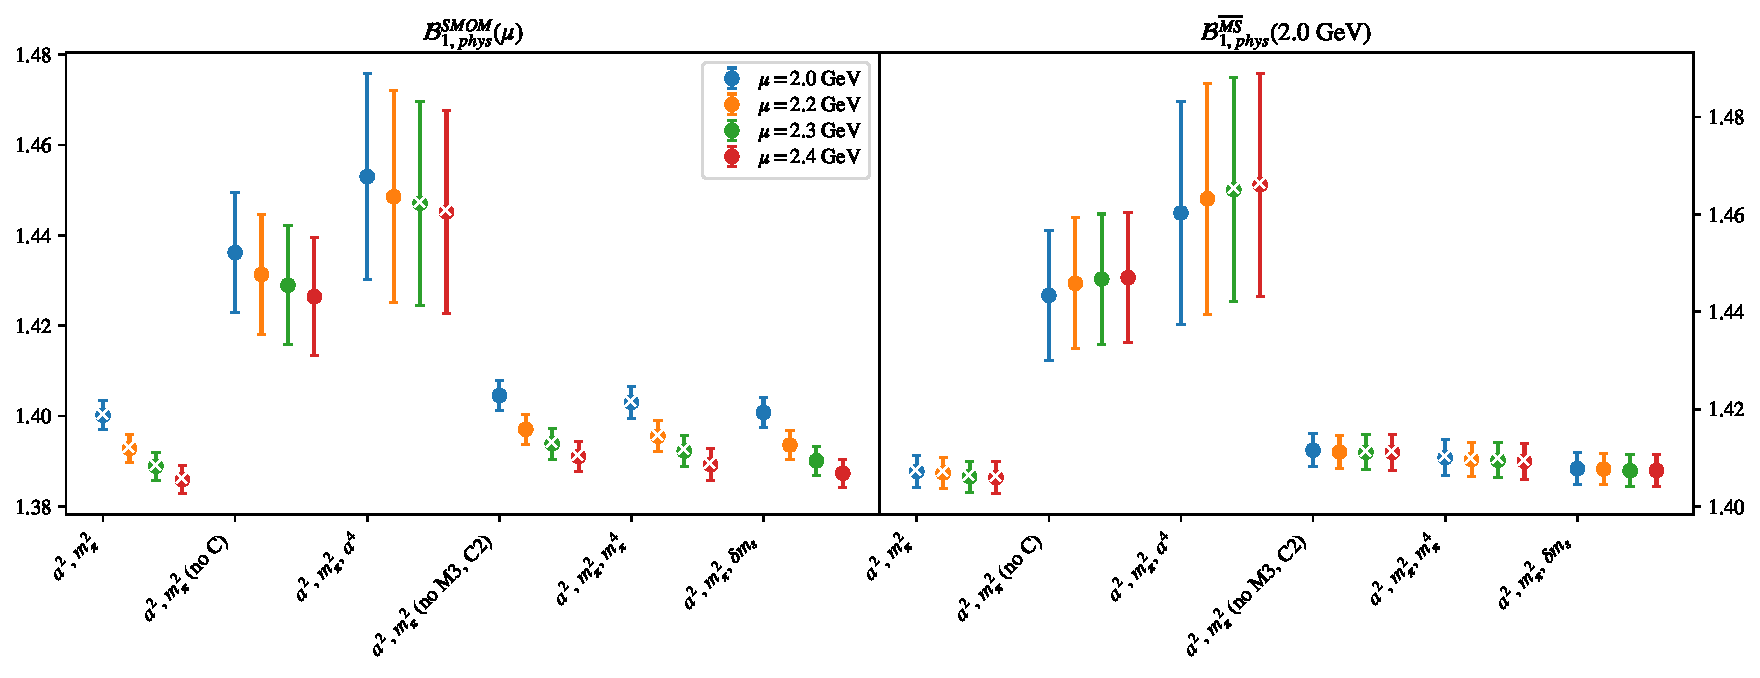
\includegraphics[page=1, width=1.1\textwidth]{VVpAA/NPR/fit_summary_bag.pdf}
\caption{$\mathcal{B}_{1}$\\(left) $\mathcal{B}_{phys}$ in RI/SMOM scheme from fit variations (fits with $p$-value $<0.05$ marked with ``$\times$"). \\(right) $\mathcal{B}_{phys}$ in $\overline{MS}$ computed using $\mathcal{B}^{\overline{MS}} = R^{\overline{MS}\leftarrow SMOM}(2.0)\sigma_{npt}(2.0,\mu) \mathcal{B}^{SMOM}(\mu)$.}
\end{figure}
\clearpage
\begin{figure}
\centering
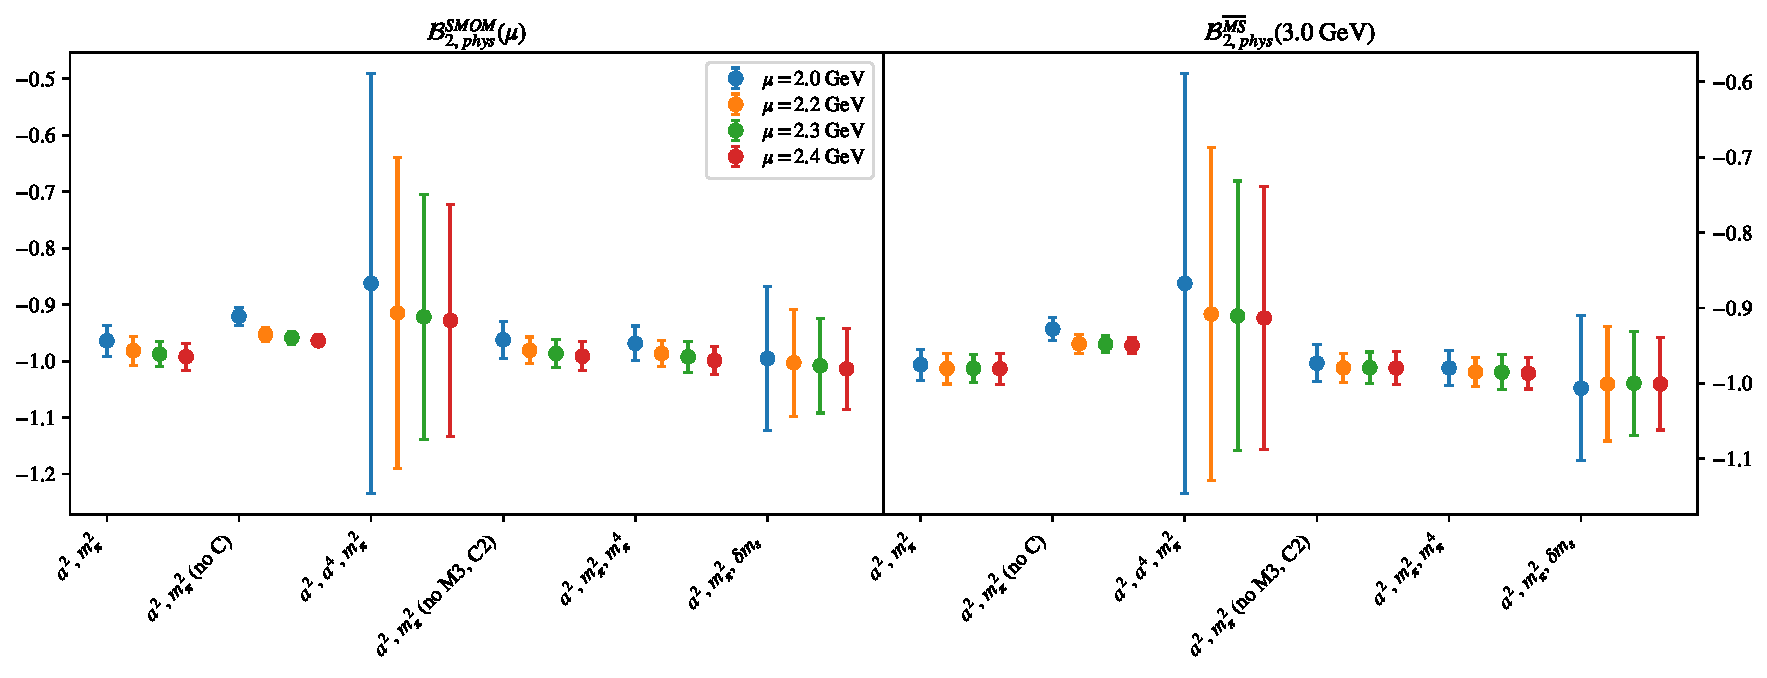
\includegraphics[page=1, width=1.1\textwidth]{VVmAA/NPR/fit_summary_bag.pdf}
\caption{$\mathcal{B}_{2}$\\(left) $\mathcal{B}_{phys}$ in RI/SMOM scheme from fit variations (fits with $p$-value $<0.05$ marked with ``$\times$"). \\(right) $\mathcal{B}_{phys}$ in $\overline{MS}$ computed using $\mathcal{B}^{\overline{MS}} = R^{\overline{MS}\leftarrow SMOM}(3.0)\sigma_{npt}(3.0,\mu) \mathcal{B}^{SMOM}(\mu)$.}
\end{figure}
\clearpage
\begin{figure}
\centering
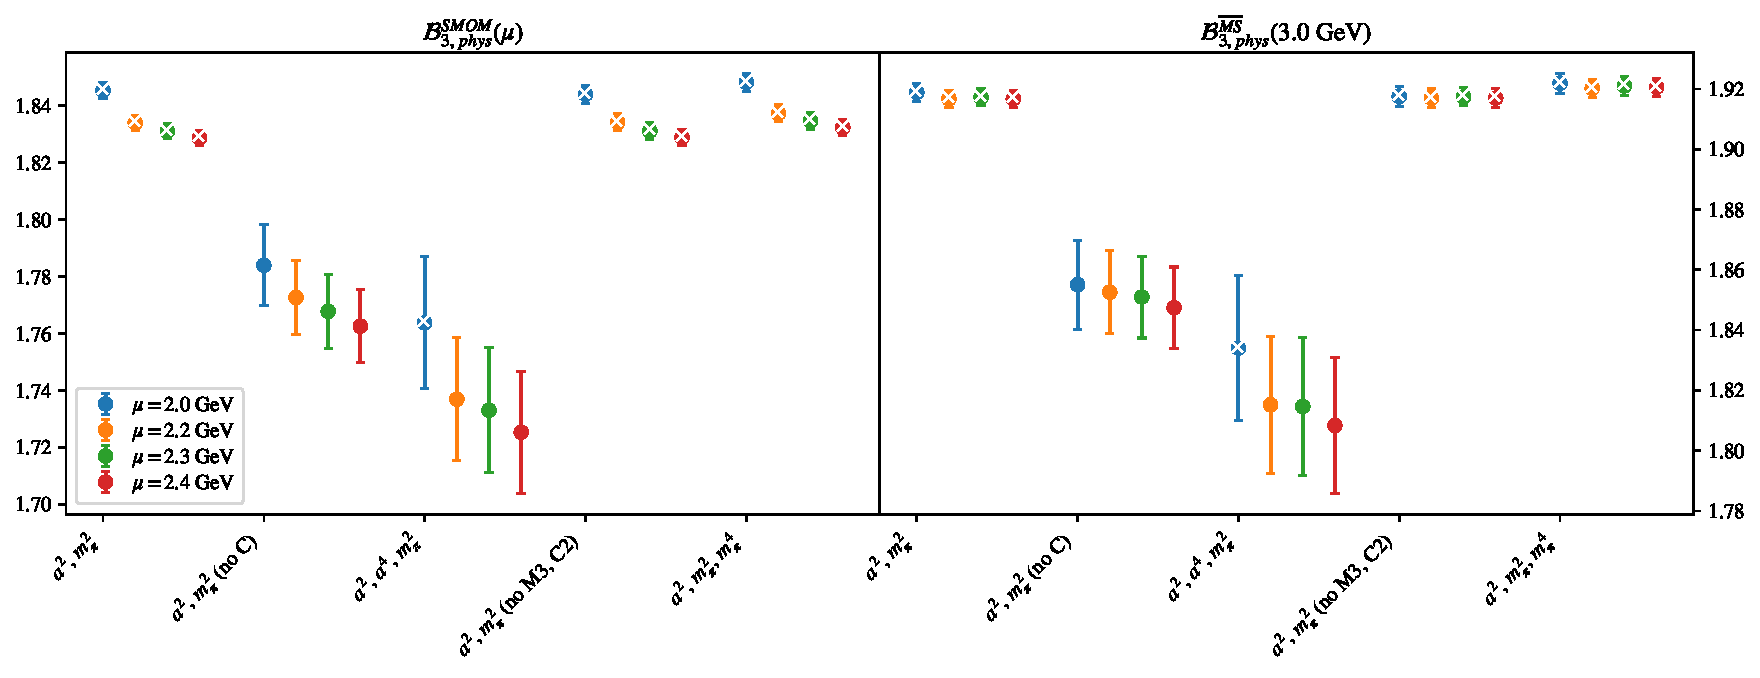
\includegraphics[page=1, width=1.1\textwidth]{SSmPP/NPR/fit_summary_bag.pdf}
\caption{$\mathcal{B}_{3}$\\(left) $\mathcal{B}_{phys}$ in RI/SMOM scheme from fit variations (fits with $p$-value $<0.05$ marked with ``$\times$"). \\(right) $\mathcal{B}_{phys}$ in $\overline{MS}$ computed using $\mathcal{B}^{\overline{MS}} = R^{\overline{MS}\leftarrow SMOM}(3.0)\sigma_{npt}(3.0,\mu) \mathcal{B}^{SMOM}(\mu)$.}
\end{figure}
\clearpage
\begin{figure}
\centering
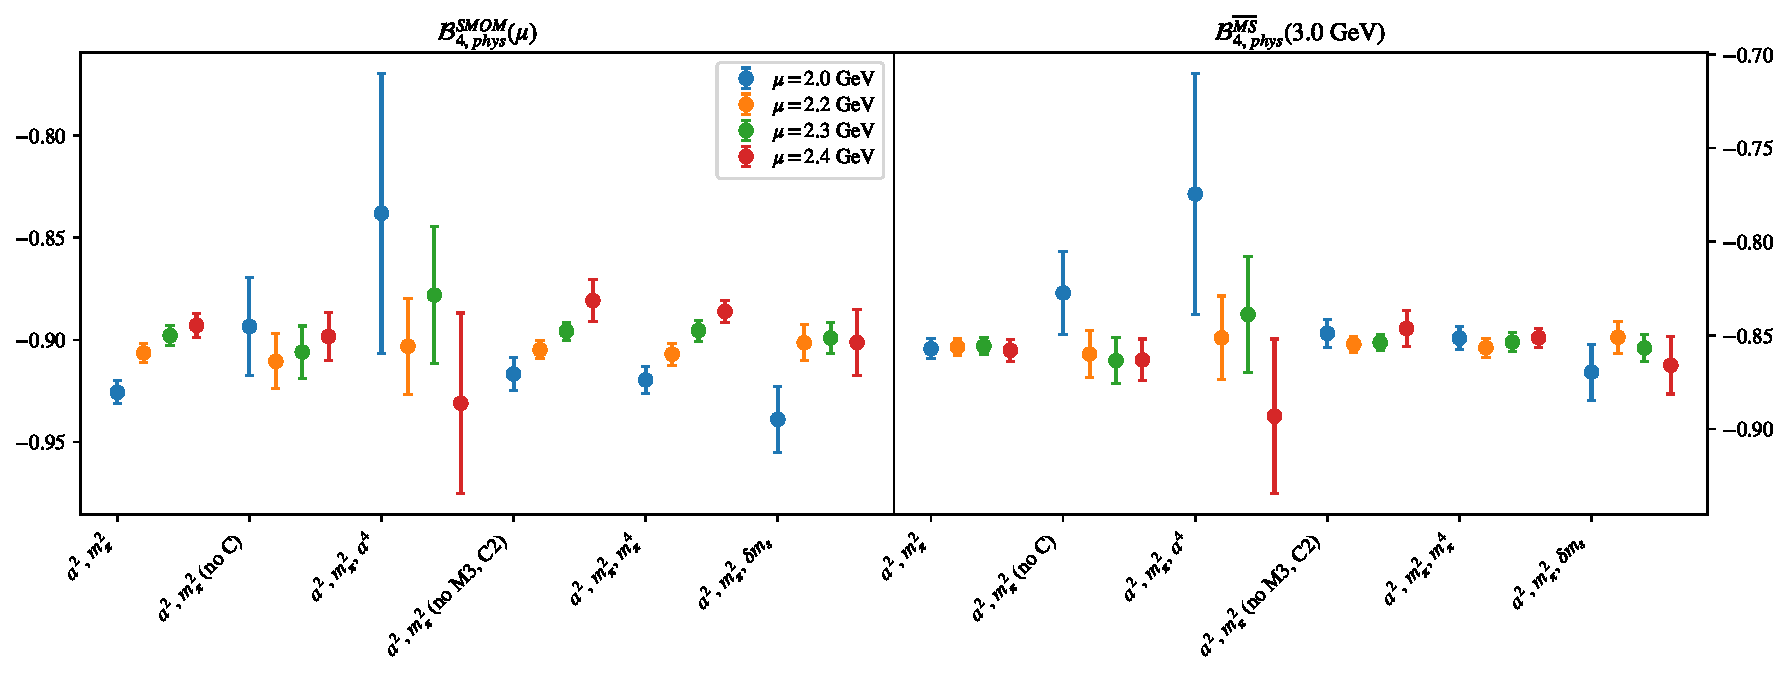
\includegraphics[page=1, width=1.1\textwidth]{SSpPP/NPR/fit_summary_bag.pdf}
\caption{$\mathcal{B}_{4}$\\(left) $\mathcal{B}_{phys}$ in RI/SMOM scheme from fit variations (fits with $p$-value $<0.05$ marked with ``$\times$"). \\(right) $\mathcal{B}_{phys}$ in $\overline{MS}$ computed using $\mathcal{B}^{\overline{MS}} = R^{\overline{MS}\leftarrow SMOM}(3.0)\sigma_{npt}(3.0,\mu) \mathcal{B}^{SMOM}(\mu)$.}
\end{figure}
\clearpage
\begin{figure}
\centering
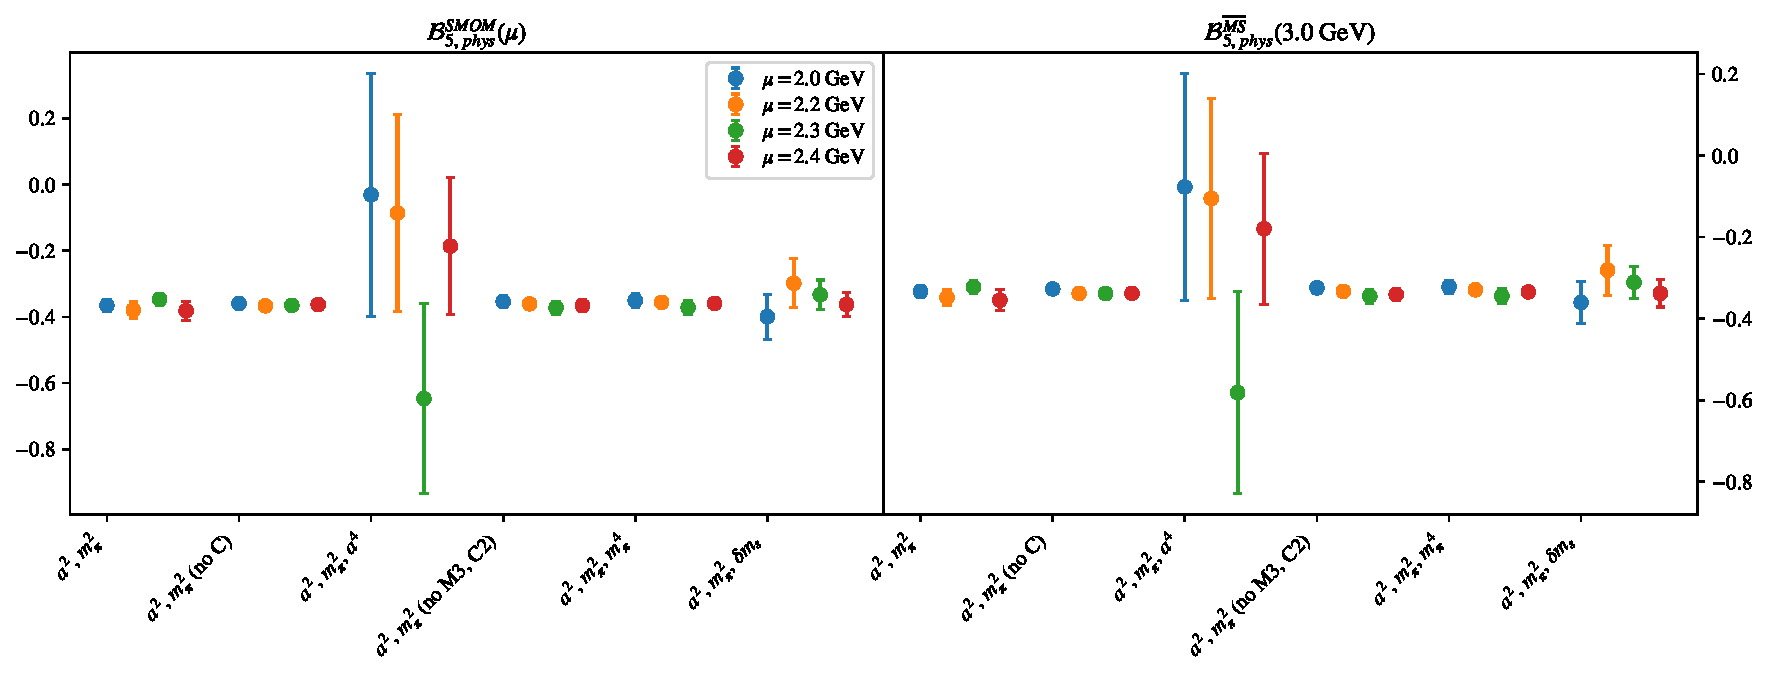
\includegraphics[page=1, width=1.1\textwidth]{TT/NPR/fit_summary_bag.pdf}
\caption{$\mathcal{B}_{5}$\\(left) $\mathcal{B}_{phys}$ in RI/SMOM scheme from fit variations (fits with $p$-value $<0.05$ marked with ``$\times$"). \\(right) $\mathcal{B}_{phys}$ in $\overline{MS}$ computed using $\mathcal{B}^{\overline{MS}} = R^{\overline{MS}\leftarrow SMOM}(3.0)\sigma_{npt}(3.0,\mu) \mathcal{B}^{SMOM}(\mu)$.}
\end{figure}
\clearpage
\section{$\mathcal{B}_1$}
\begin{table}[h!]
\begin{center}
\begin{tabular}{|c|c|c|c|c|c|}
\hline
$\mu$ (GeV) & $a^2$, $m_\pi^2$& $a^2$, $m_\pi^2$ (no C)& $a^2$, $a^4$, $m_\pi^2$& $a^2$, $m_\pi^2$ (no M3, C2)& $a^2$, $m_\pi^2$, $m_\pi^4$\\
\hline
2.0& \hyperlink{VVpAA/NPR/a2m2_20.pdf.1}{\textbf{1.4022(28)}: 2.239 (0.048)} & \hyperlink{VVpAA/NPR/a2m2noC_20.pdf.1}{\textbf{1.416(13)}: 0.876 (0.417)} & \hyperlink{VVpAA/NPR/a2a4m2_20.pdf.1}{\textbf{1.417(22)}: 2.681 (0.03)} & \hyperlink{VVpAA/NPR/a2m2mcut_20.pdf.1}{\textbf{1.4080(33)}: 0.273 (0.845)} & \hyperlink{VVpAA/NPR/a2m2m4_20.pdf.1}{\textbf{1.4077(34)}: 1.137 (0.337)}\\
2.2& \hyperlink{VVpAA/NPR/a2m2_22.pdf.1}{\textbf{1.3949(27)}: 2.636 (0.022)} & \hyperlink{VVpAA/NPR/a2m2noC_22.pdf.1}{\textbf{1.411(12)}: 1.11 (0.329)} & \hyperlink{VVpAA/NPR/a2a4m2_22.pdf.1}{\textbf{1.413(21)}: 3.094 (0.015)} & \hyperlink{VVpAA/NPR/a2m2mcut_22.pdf.1}{\textbf{1.4011(33)}: 0.392 (0.759)} & \hyperlink{VVpAA/NPR/a2m2m4_22.pdf.1}{\textbf{1.4008(34)}: 1.304 (0.266)}\\
2.3& \hyperlink{VVpAA/NPR/a2m2_23.pdf.1}{\textbf{1.3919(27)}: 2.615 (0.023)} & \hyperlink{VVpAA/NPR/a2m2noC_23.pdf.1}{\textbf{1.408(12)}: 1.159 (0.314)} & \hyperlink{VVpAA/NPR/a2a4m2_23.pdf.1}{\textbf{1.412(21)}: 3.034 (0.016)} & \hyperlink{VVpAA/NPR/a2m2mcut_23.pdf.1}{\textbf{1.3979(33)}: 0.448 (0.719)} & \hyperlink{VVpAA/NPR/a2m2m4_23.pdf.1}{\textbf{1.3977(34)}: 1.351 (0.248)}\\
2.4& \hyperlink{VVpAA/NPR/a2m2_24.pdf.1}{\textbf{1.3889(27)}: 2.796 (0.016)} & \hyperlink{VVpAA/NPR/a2m2noC_24.pdf.1}{\textbf{1.405(12)}: 1.218 (0.296)} & \hyperlink{VVpAA/NPR/a2a4m2_24.pdf.1}{\textbf{1.409(21)}: 3.25 (0.011)} & \hyperlink{VVpAA/NPR/a2m2mcut_24.pdf.1}{\textbf{1.3952(32)}: 0.456 (0.713)} & \hyperlink{VVpAA/NPR/a2m2m4_24.pdf.1}{\textbf{1.3950(33)}: 1.388 (0.235)}\\
\hline
\end{tabular}
\caption{Physical point value from chiral and continuum extrapolation at renormalisation scale $\mu$. Entries are \textbf{value(error)}: $\chi^2/\text{DOF}$ ($p$-value).}
\end{center}
\end{table}
\begin{table}[h!]
\begin{center}
\begin{tabular}{|c c|c|c|c|c|c|}
\hline
$\mu$ (GeV) &  & $a^2$, $m_\pi^2$& $a^2$, $m_\pi^2$ (no C)& $a^2$, $a^4$, $m_\pi^2$& $a^2$, $m_\pi^2$ (no M3, C2)& $a^2$, $m_\pi^2$, $m_\pi^4$\\
\hline
\multirow{2}{0.5in}{2.0} & $\alpha$ & 0.0982(76)& 0.047(54)& 0.001& 0.0840(86)& 0.0854(86)\\
 & $\beta$ & 0.00275(18)& 0.00223(28)& 0.00278(18)& 0.00200(29)& 0.00028(89)\\
\hline
\multirow{2}{0.5in}{2.2} & $\alpha$ & 0.1019(72)& 0.041(52)& -0.023& 0.0868(84)& 0.0880(84)\\
 & $\beta$ & 0.00276(17)& 0.00220(28)& 0.00279(17)& 0.00192(30)& 0.00016(91)\\
\hline
\multirow{2}{0.5in}{2.3} & $\alpha$ & 0.1026(74)& 0.039(52)& -0.031& 0.0879(85)& 0.0890(86)\\
 & $\beta$ & 0.00273(17)& 0.00220(28)& 0.00276(17)& 0.00191(30)& 0.00017(90)\\
\hline
\multirow{2}{0.5in}{2.4} & $\alpha$ & 0.1037(73)& 0.040(51)& -0.031& 0.0882(85)& 0.0893(84)\\
 & $\beta$ & 0.00275(16)& 0.00220(27)& 0.00278(16)& 0.00191(29)& 0.00012(88)\\
\hline
\end{tabular}
\caption{Fit values of coefficients in $Q = Q_{phys} + \mathbf{\alpha} a^2 + \mathbf{\beta}\left(\frac{m_\pi^2}{f_\pi^2}-\frac{m_{\pi,PDG}^2}{f_\pi^2}\right) + \ldots$.}
\end{center}
\end{table}
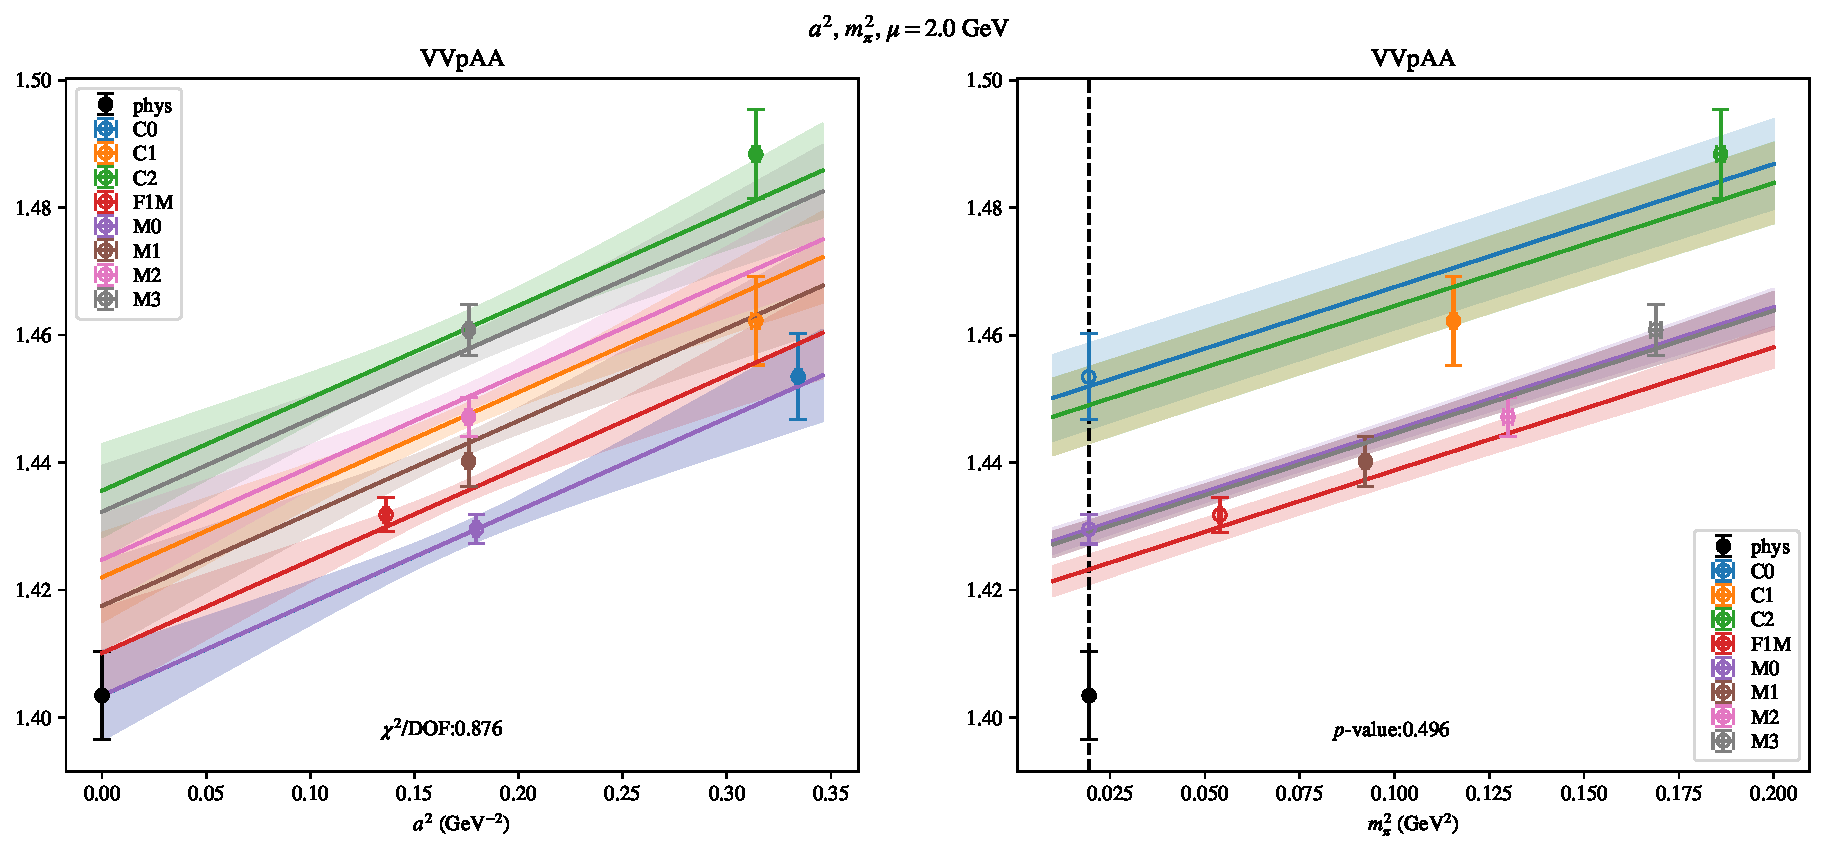
\includepdf[link, pages=-]{VVpAA/NPR/a2m2_20.pdf}
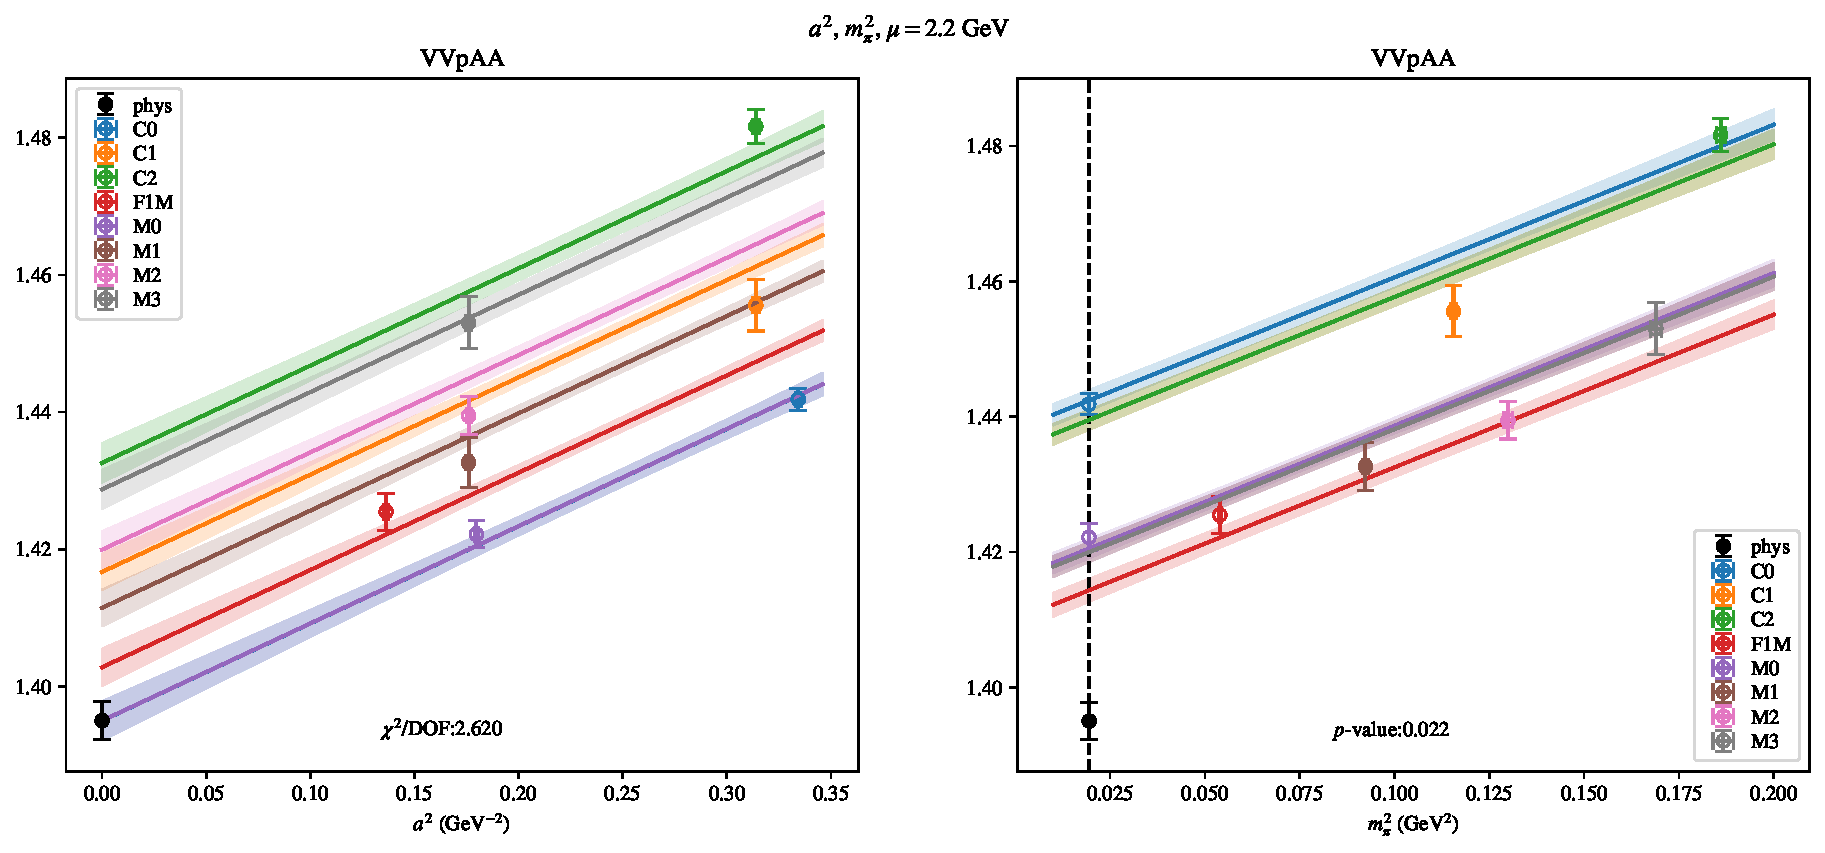
\includepdf[link, pages=-]{VVpAA/NPR/a2m2_22.pdf}
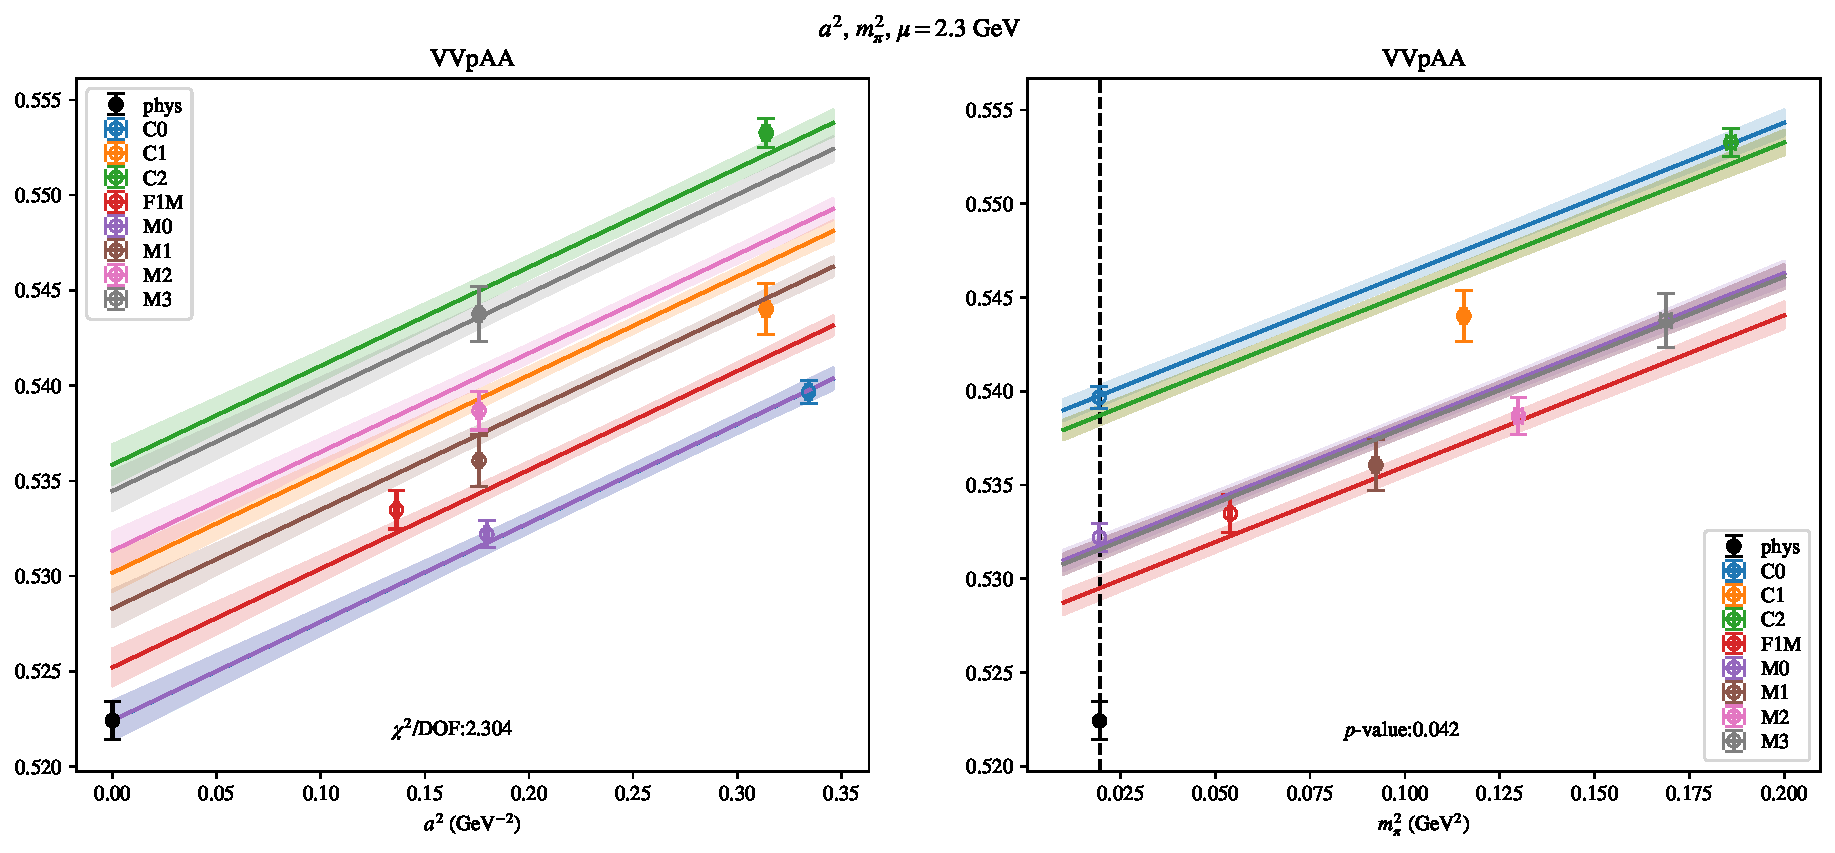
\includepdf[link, pages=-]{VVpAA/NPR/a2m2_23.pdf}
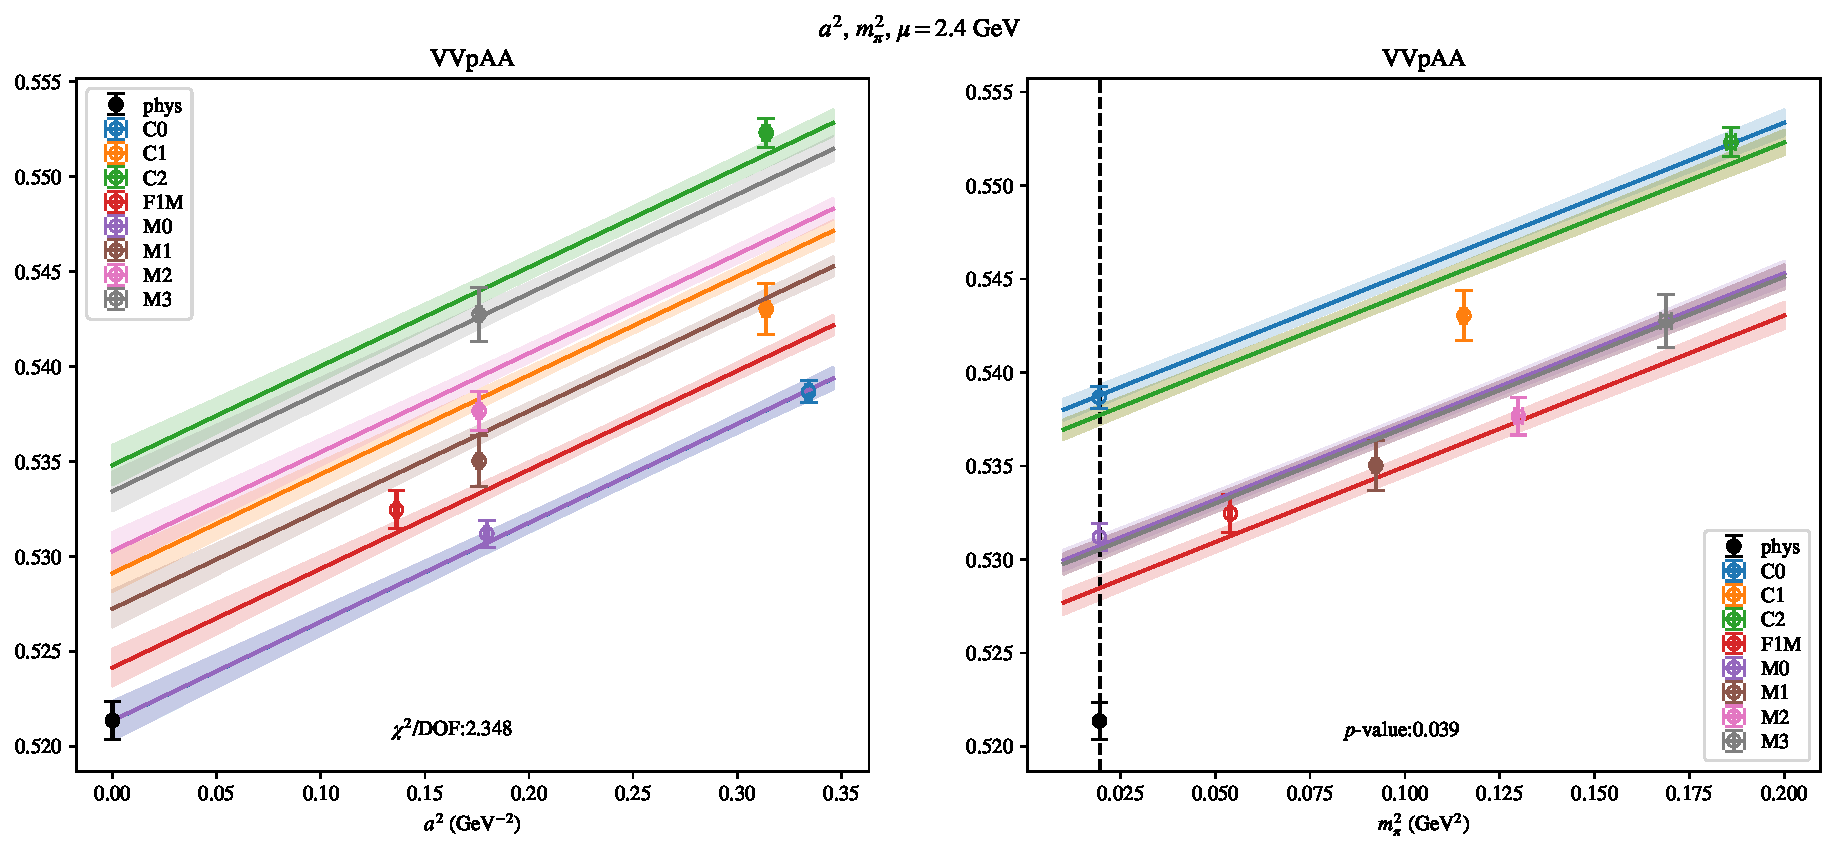
\includepdf[link, pages=-]{VVpAA/NPR/a2m2_24.pdf}
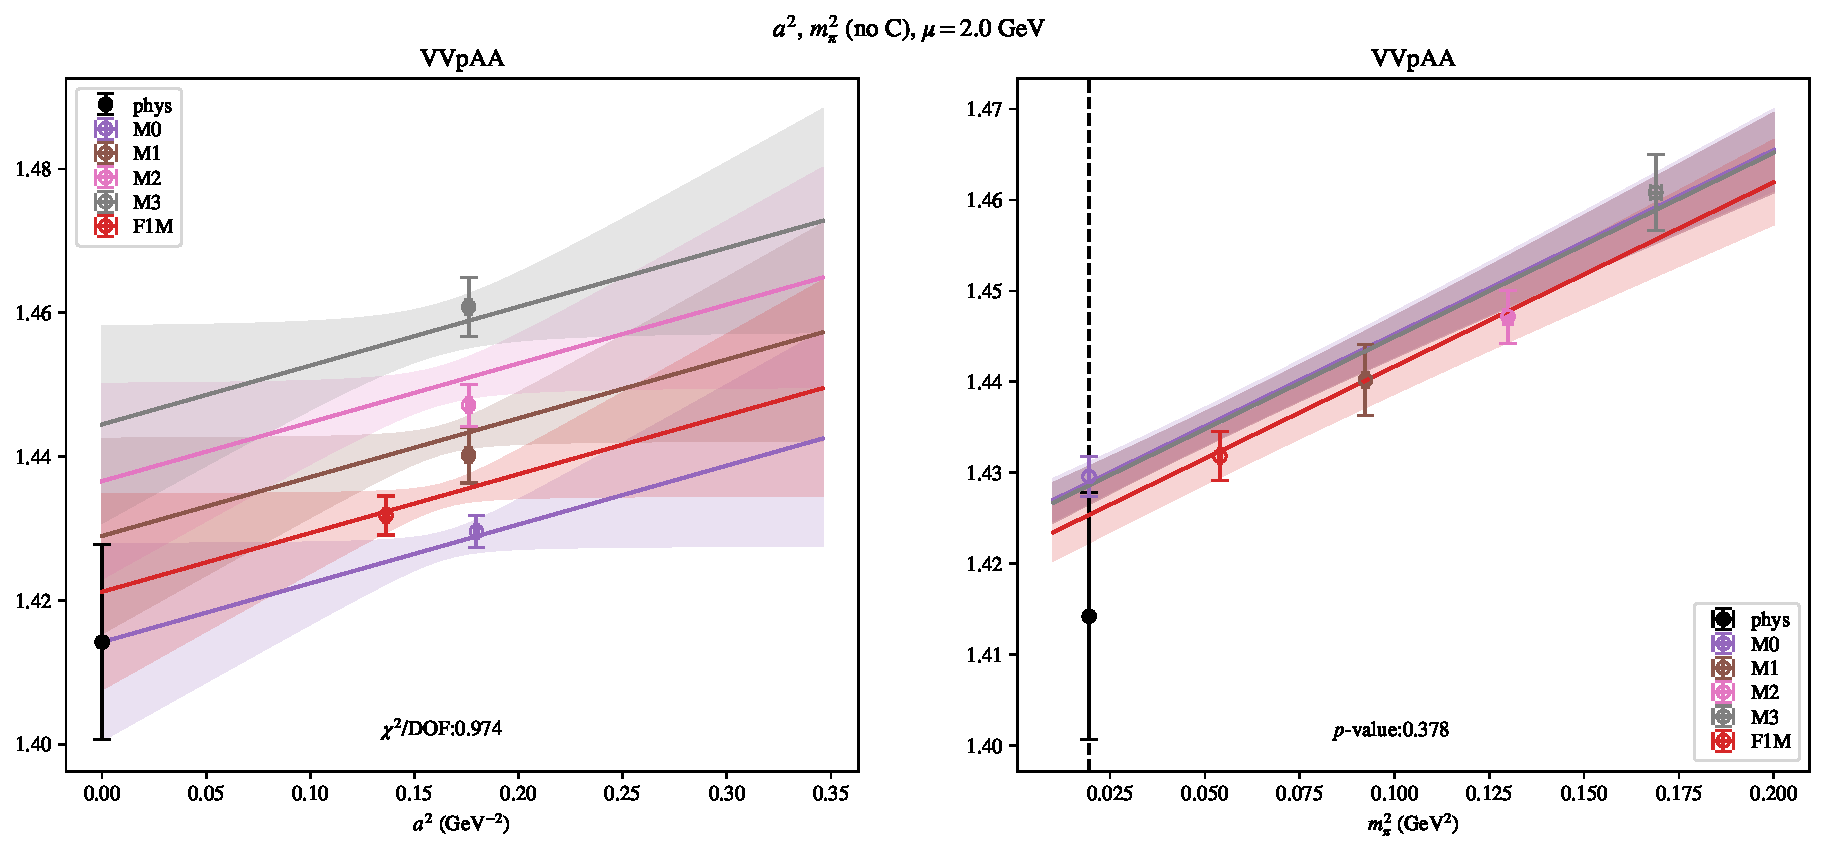
\includepdf[link, pages=-]{VVpAA/NPR/a2m2noC_20.pdf}
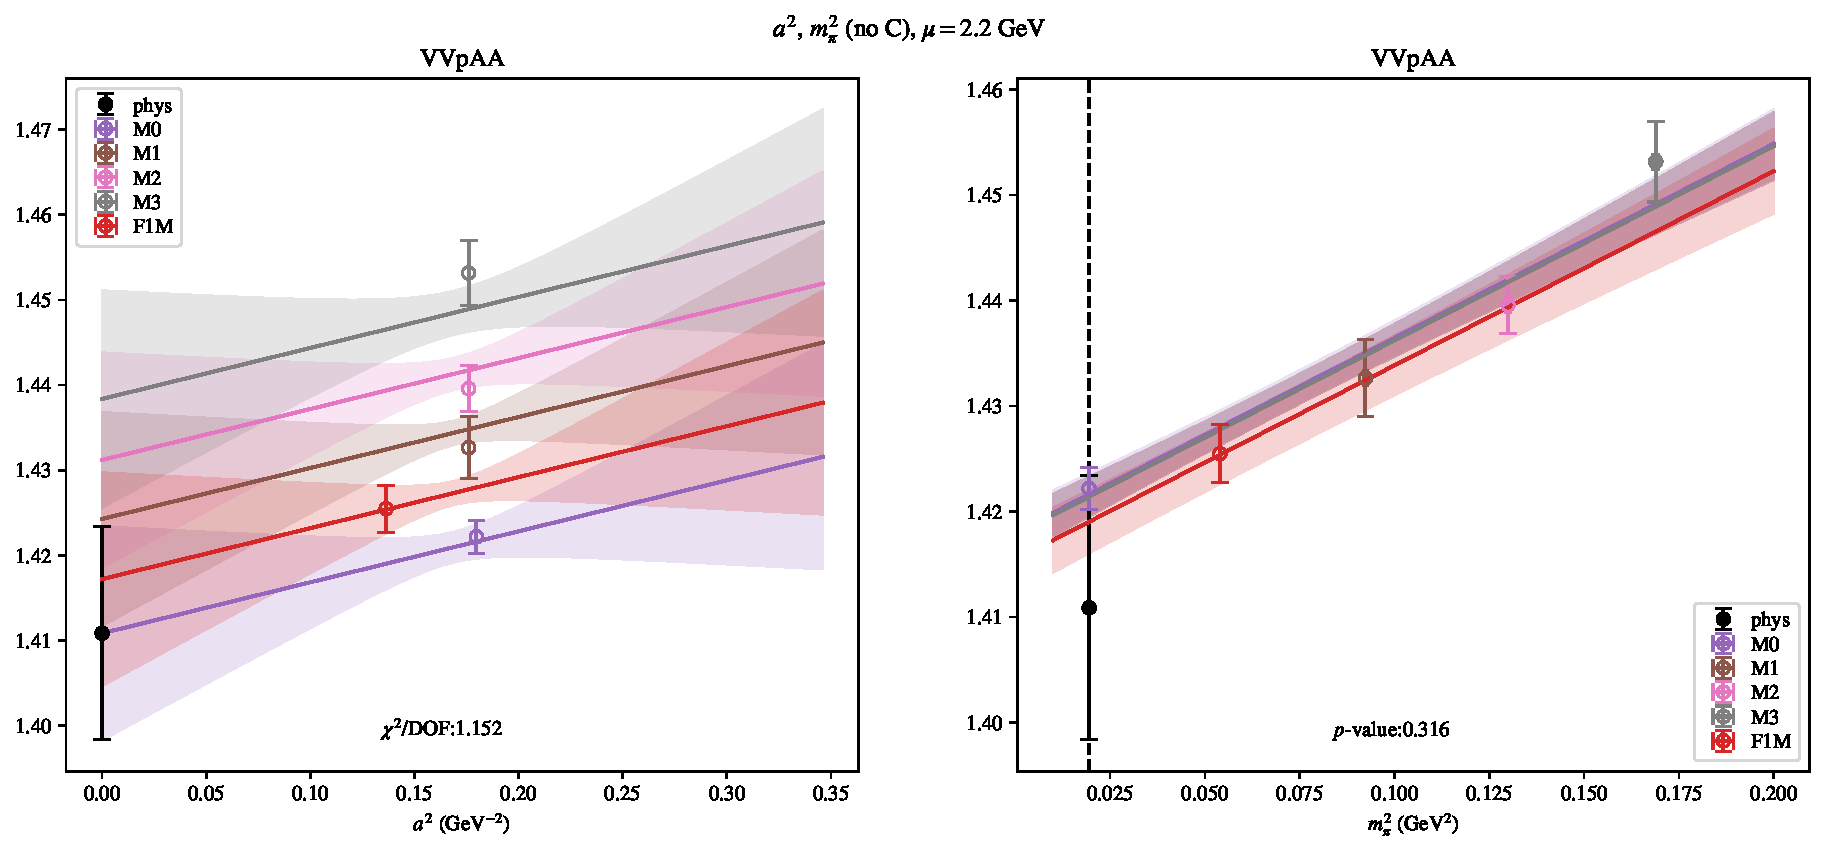
\includepdf[link, pages=-]{VVpAA/NPR/a2m2noC_22.pdf}
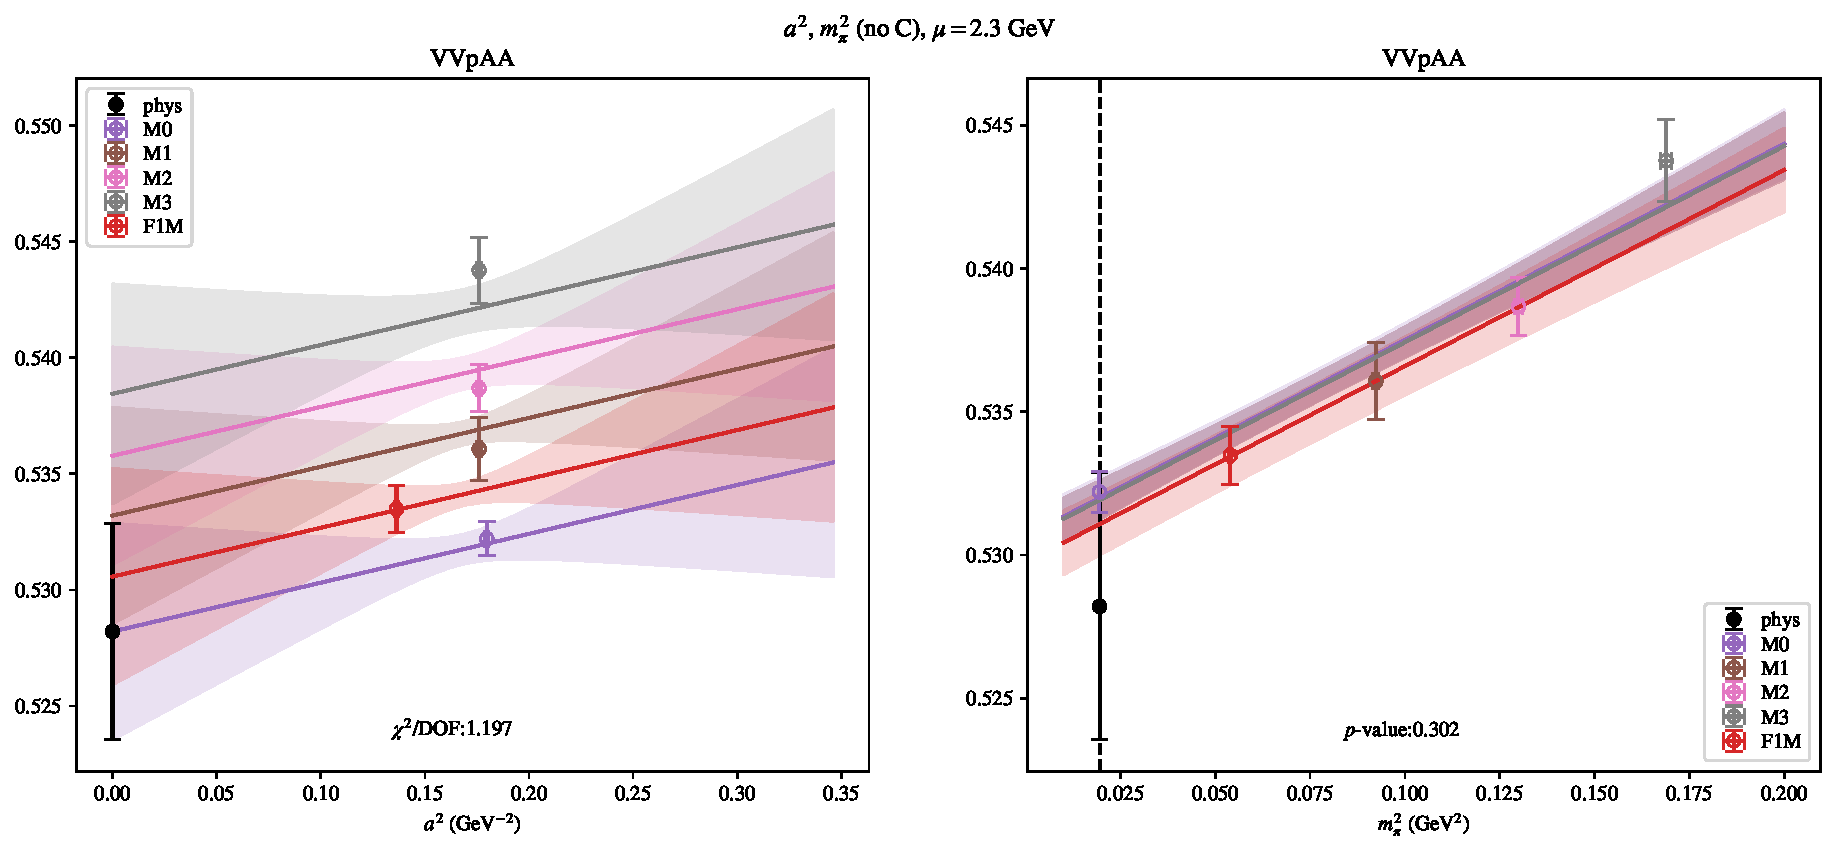
\includepdf[link, pages=-]{VVpAA/NPR/a2m2noC_23.pdf}
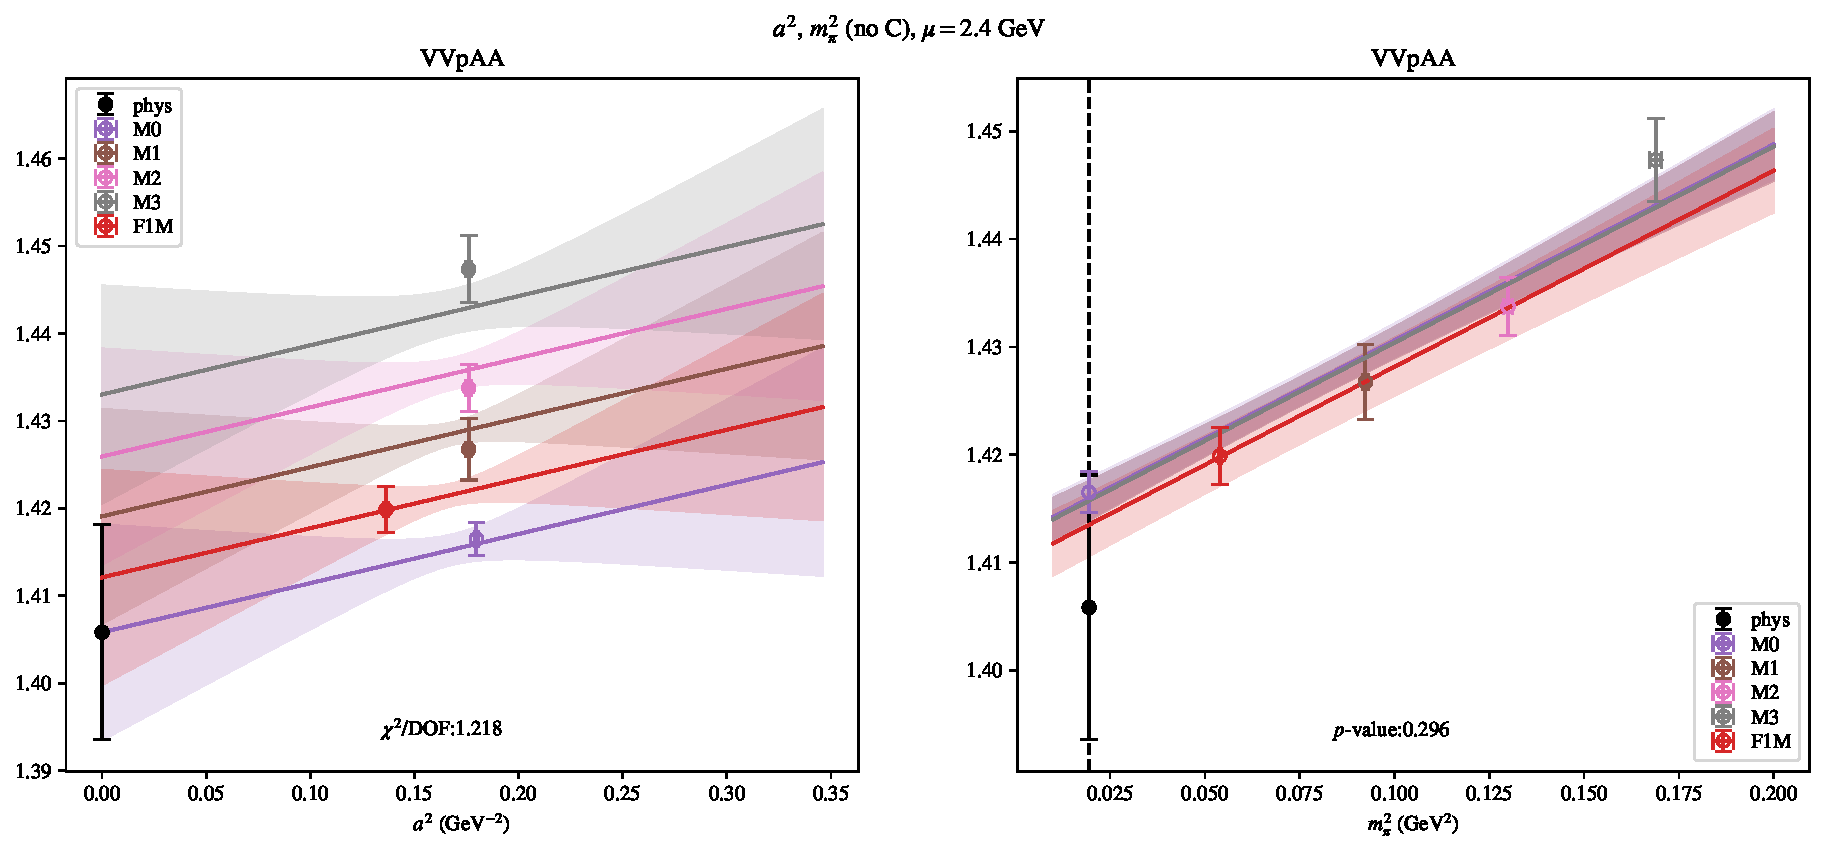
\includepdf[link, pages=-]{VVpAA/NPR/a2m2noC_24.pdf}
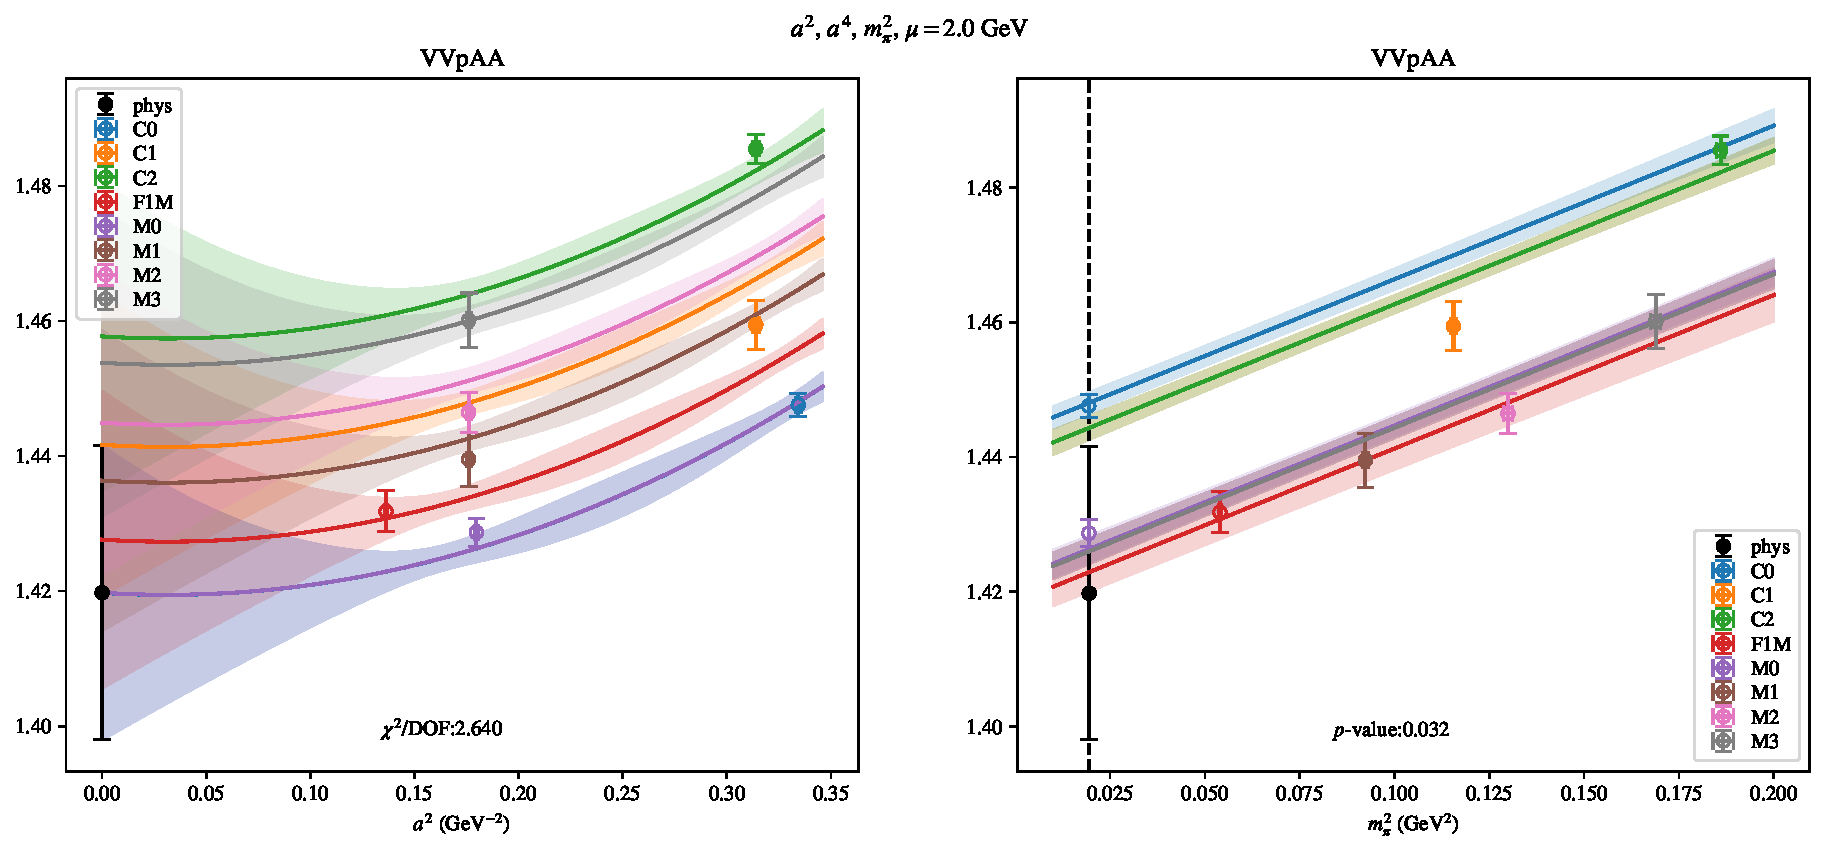
\includepdf[link, pages=-]{VVpAA/NPR/a2a4m2_20.pdf}
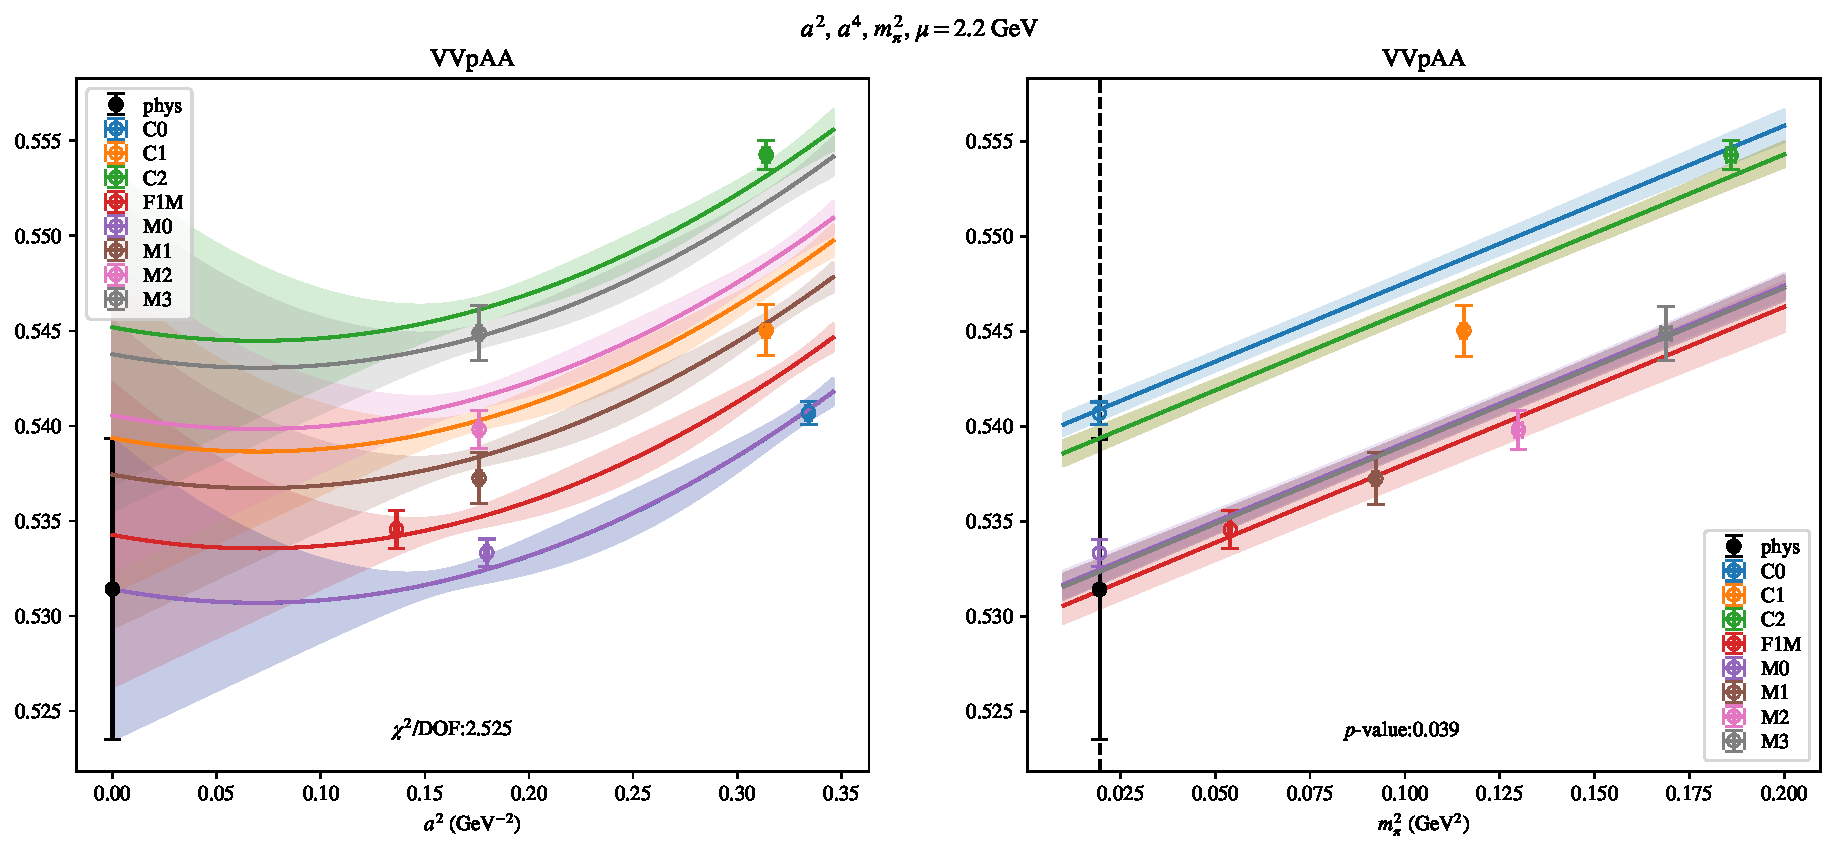
\includepdf[link, pages=-]{VVpAA/NPR/a2a4m2_22.pdf}
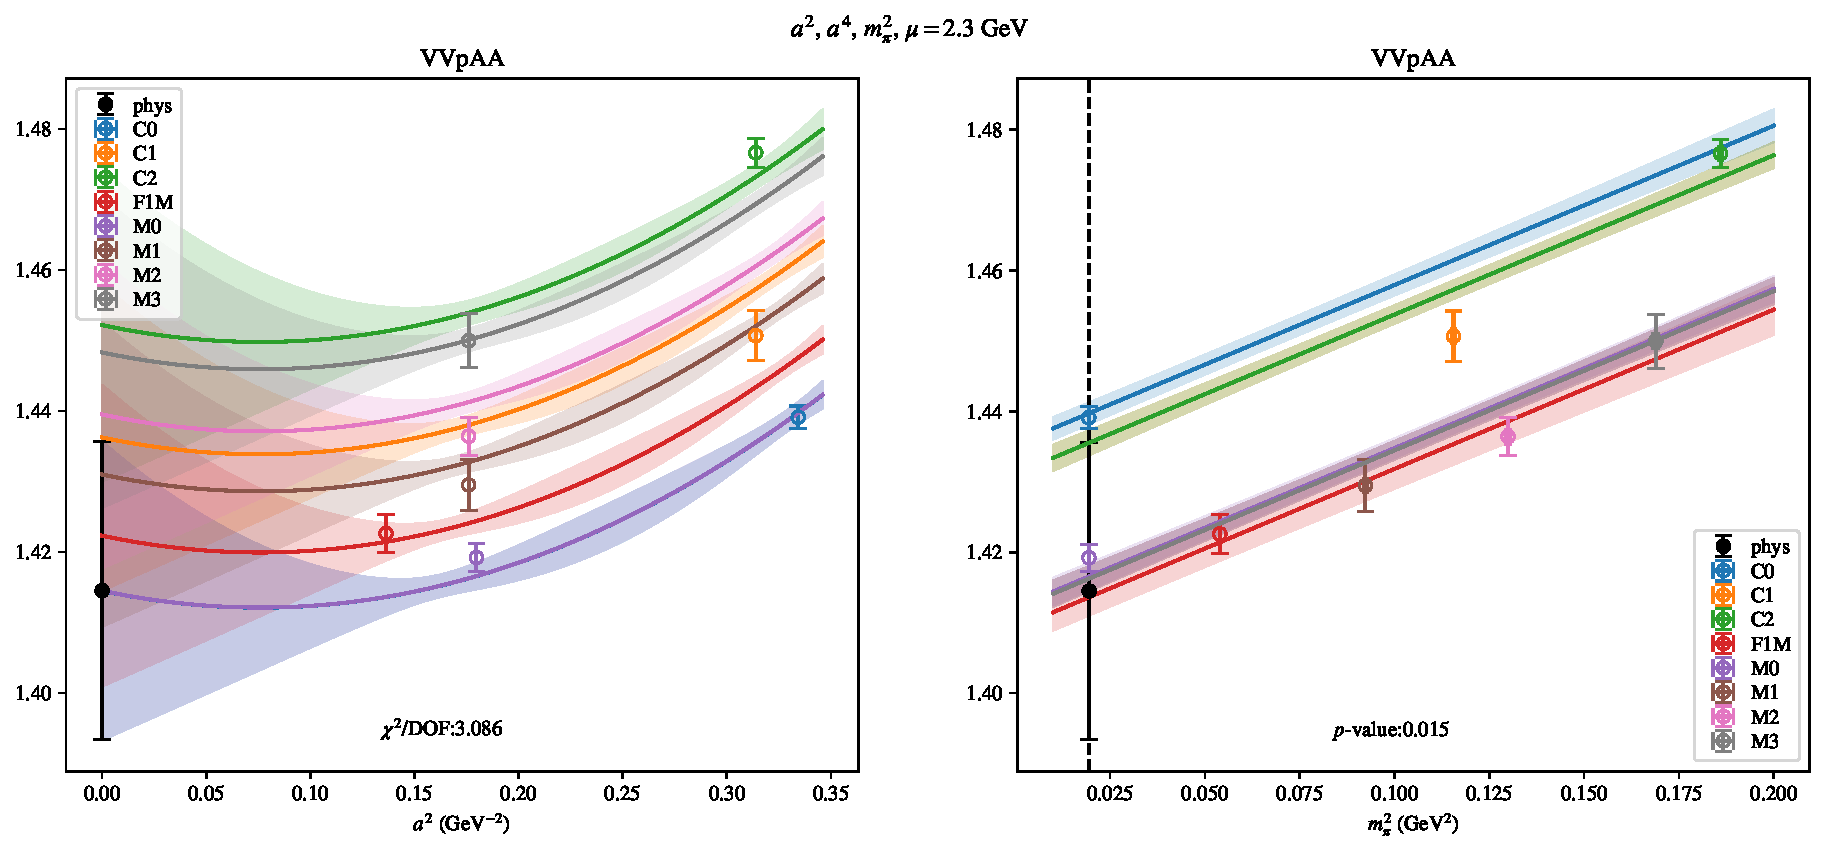
\includepdf[link, pages=-]{VVpAA/NPR/a2a4m2_23.pdf}
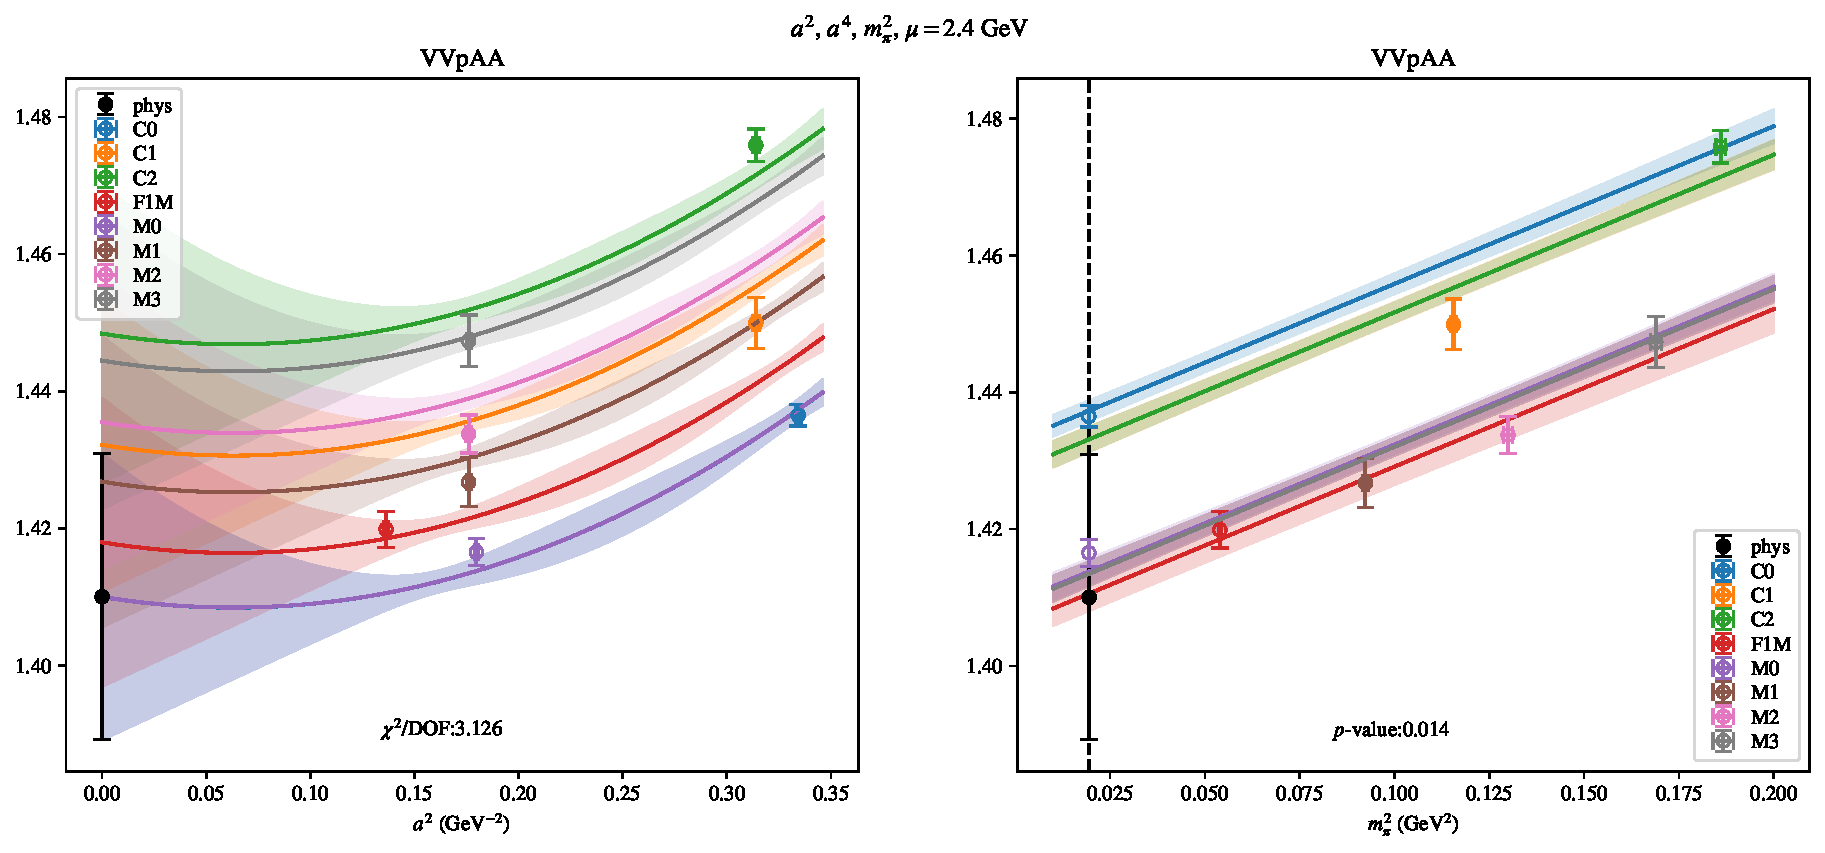
\includepdf[link, pages=-]{VVpAA/NPR/a2a4m2_24.pdf}
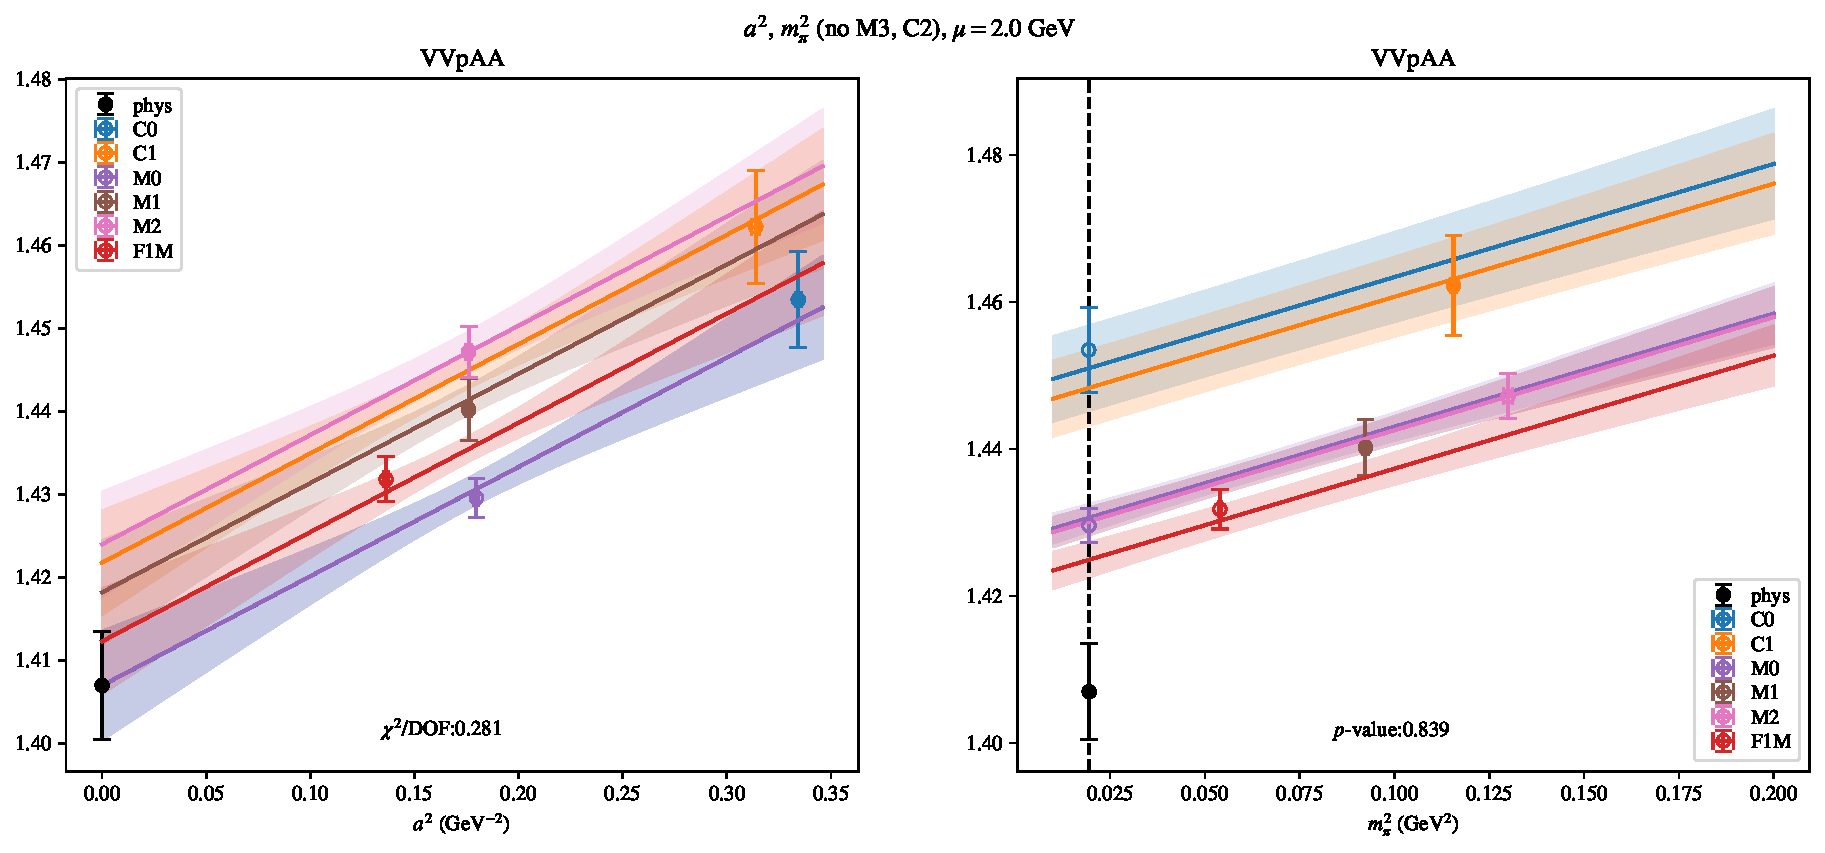
\includepdf[link, pages=-]{VVpAA/NPR/a2m2mcut_20.pdf}
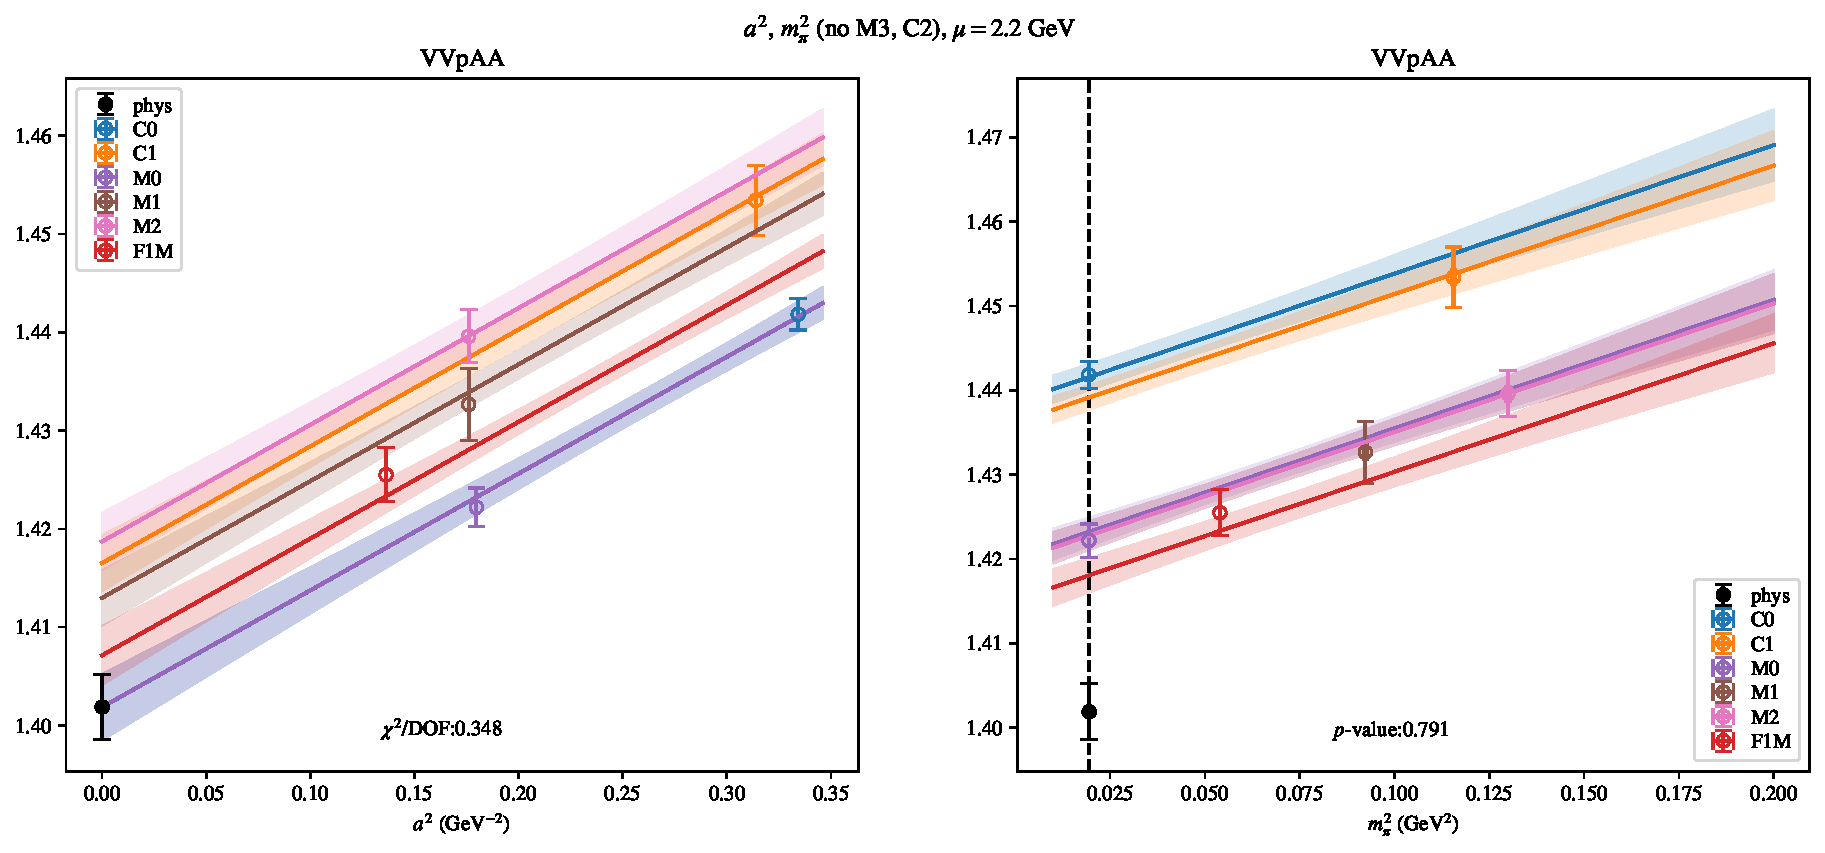
\includepdf[link, pages=-]{VVpAA/NPR/a2m2mcut_22.pdf}
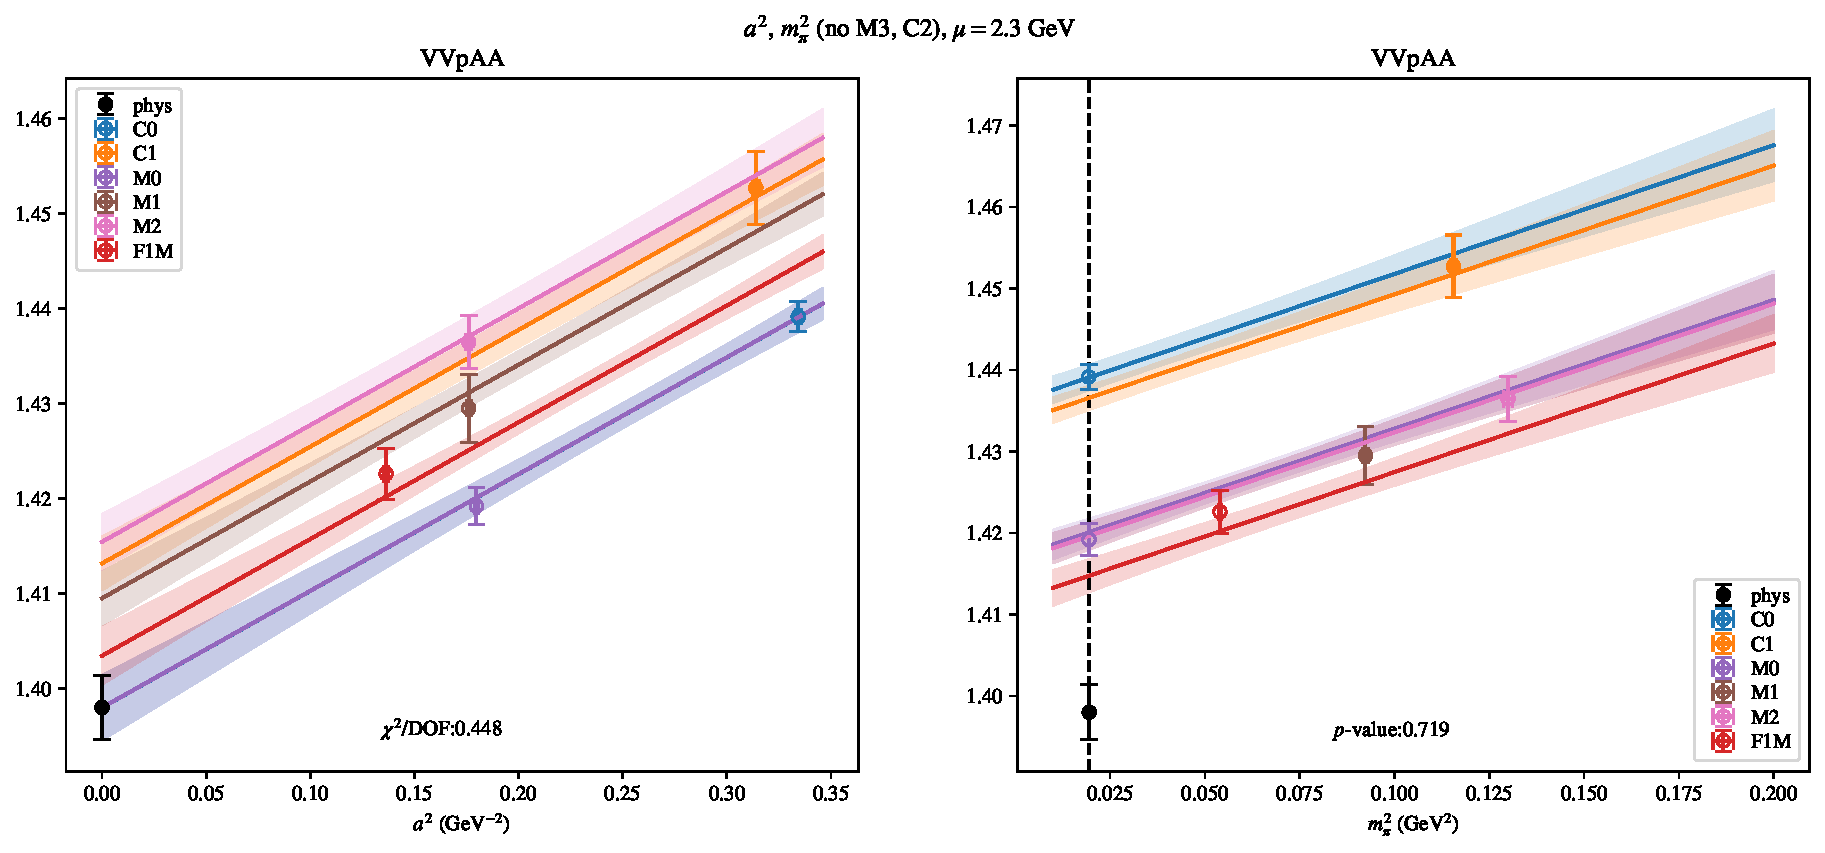
\includepdf[link, pages=-]{VVpAA/NPR/a2m2mcut_23.pdf}
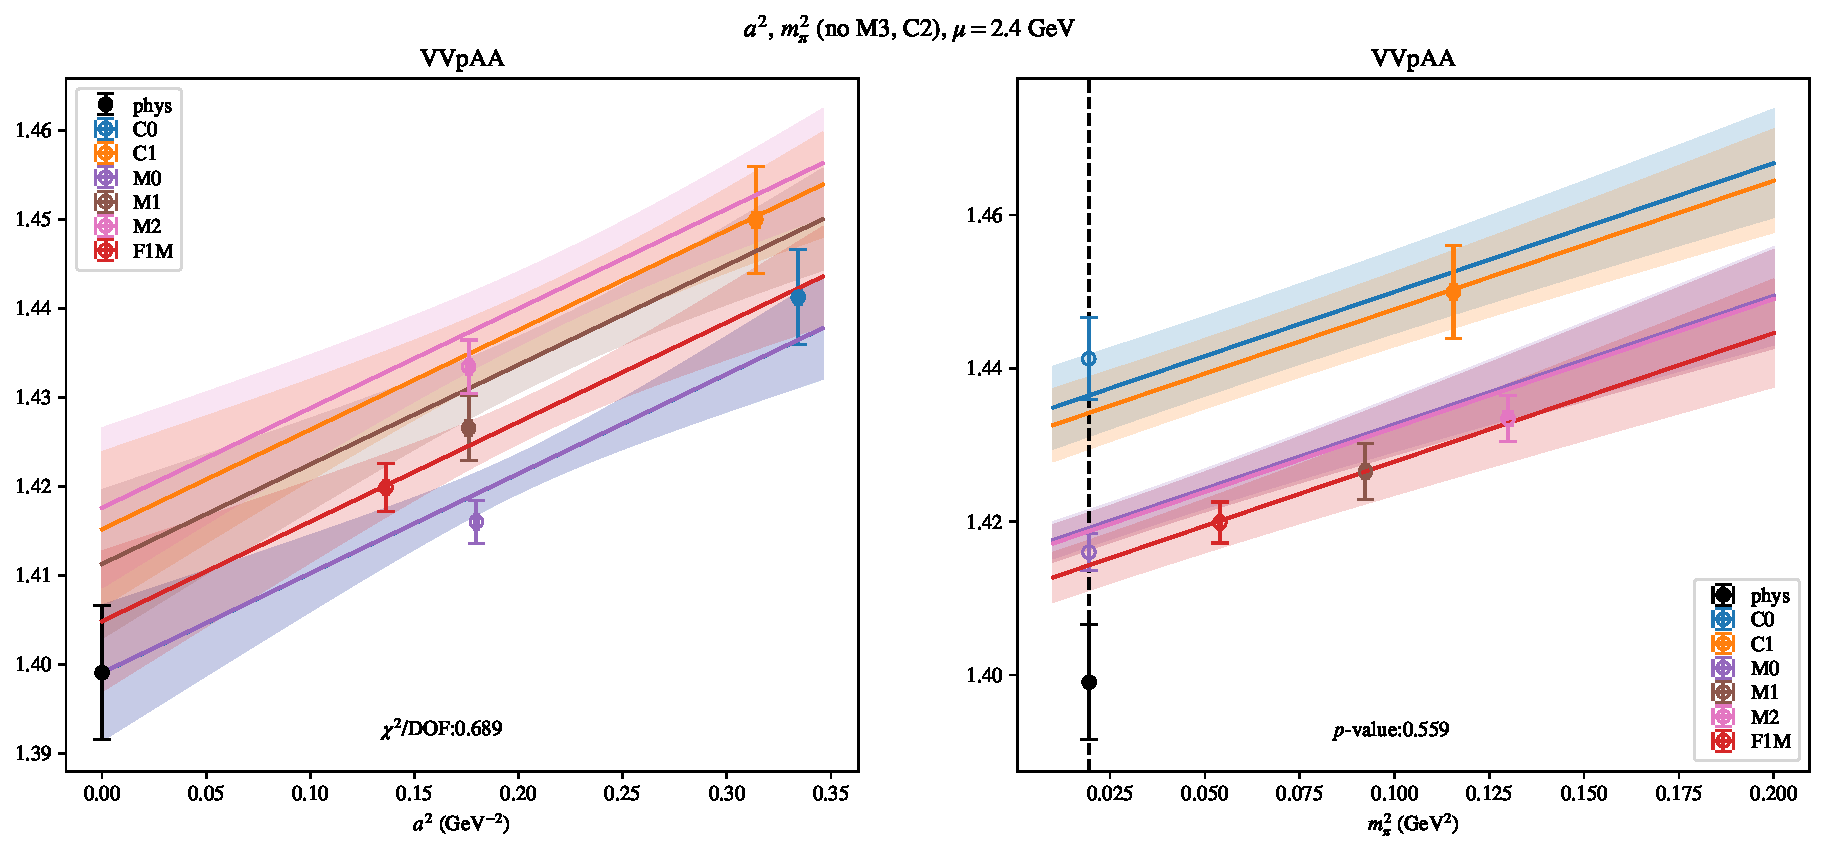
\includepdf[link, pages=-]{VVpAA/NPR/a2m2mcut_24.pdf}
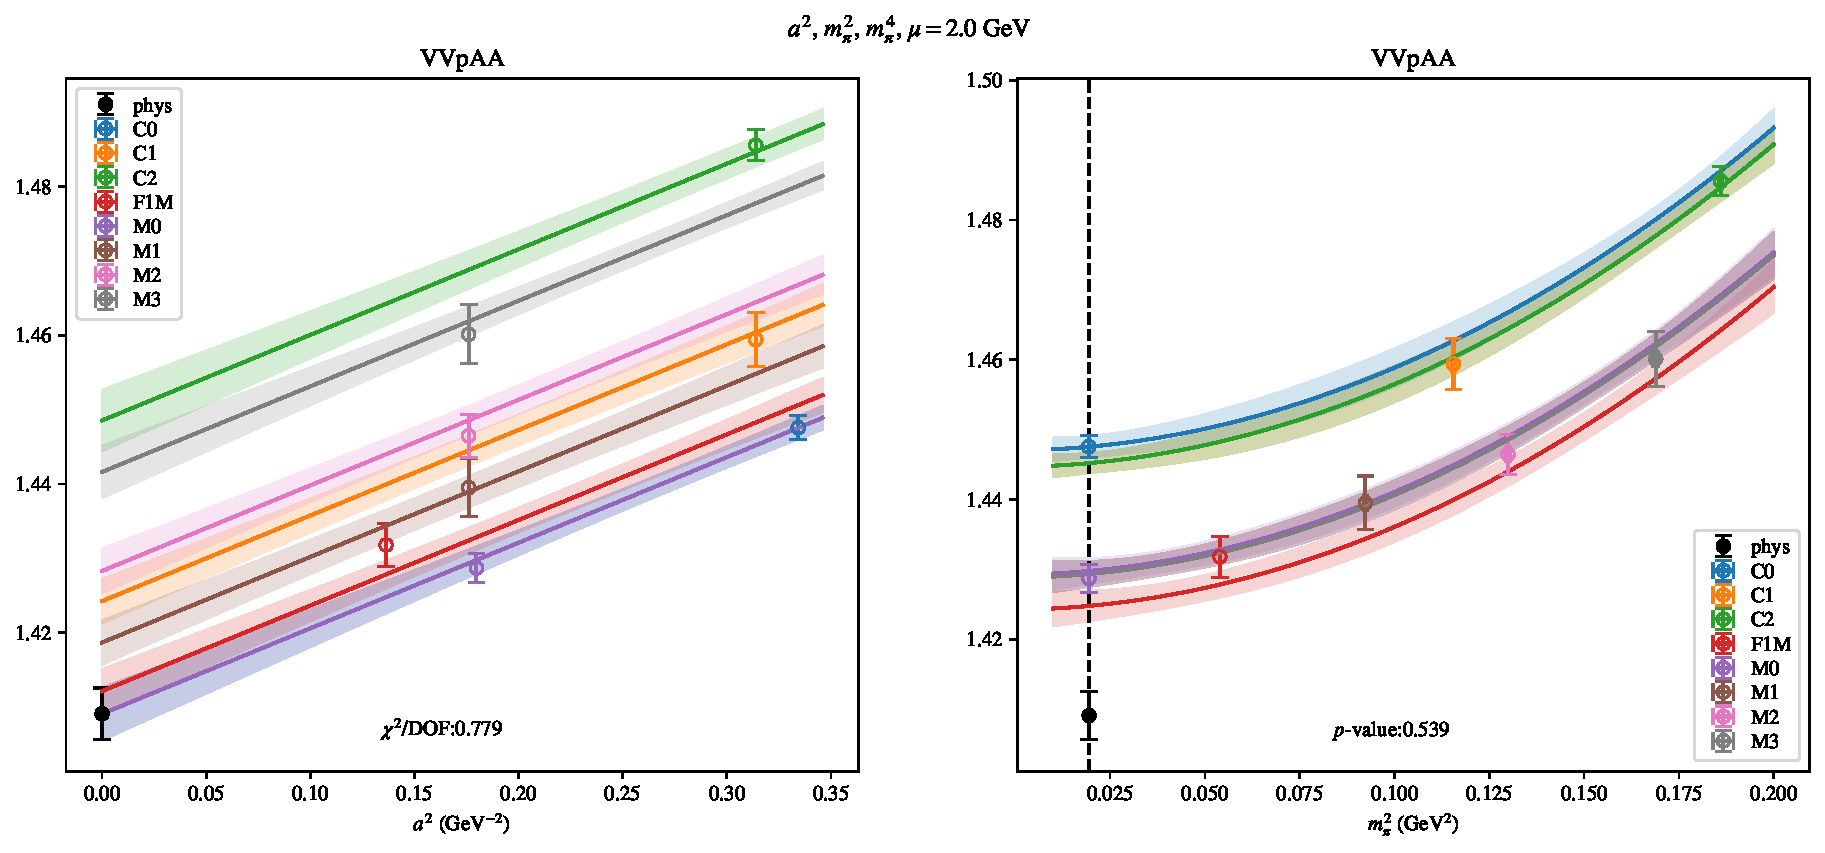
\includepdf[link, pages=-]{VVpAA/NPR/a2m2m4_20.pdf}
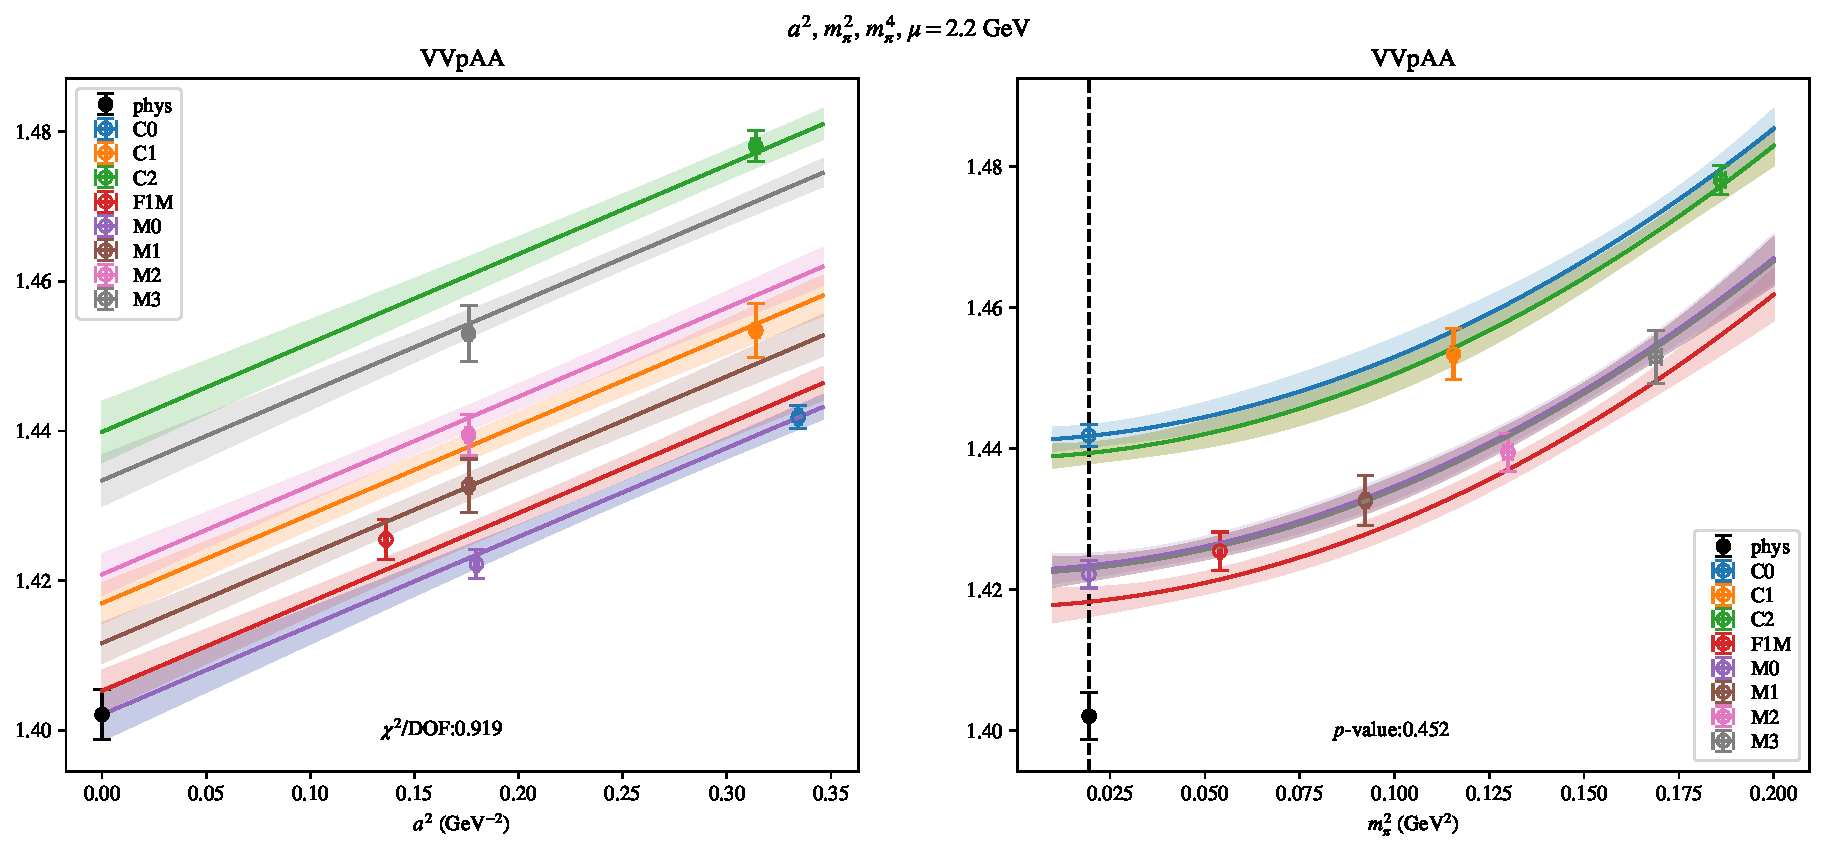
\includepdf[link, pages=-]{VVpAA/NPR/a2m2m4_22.pdf}
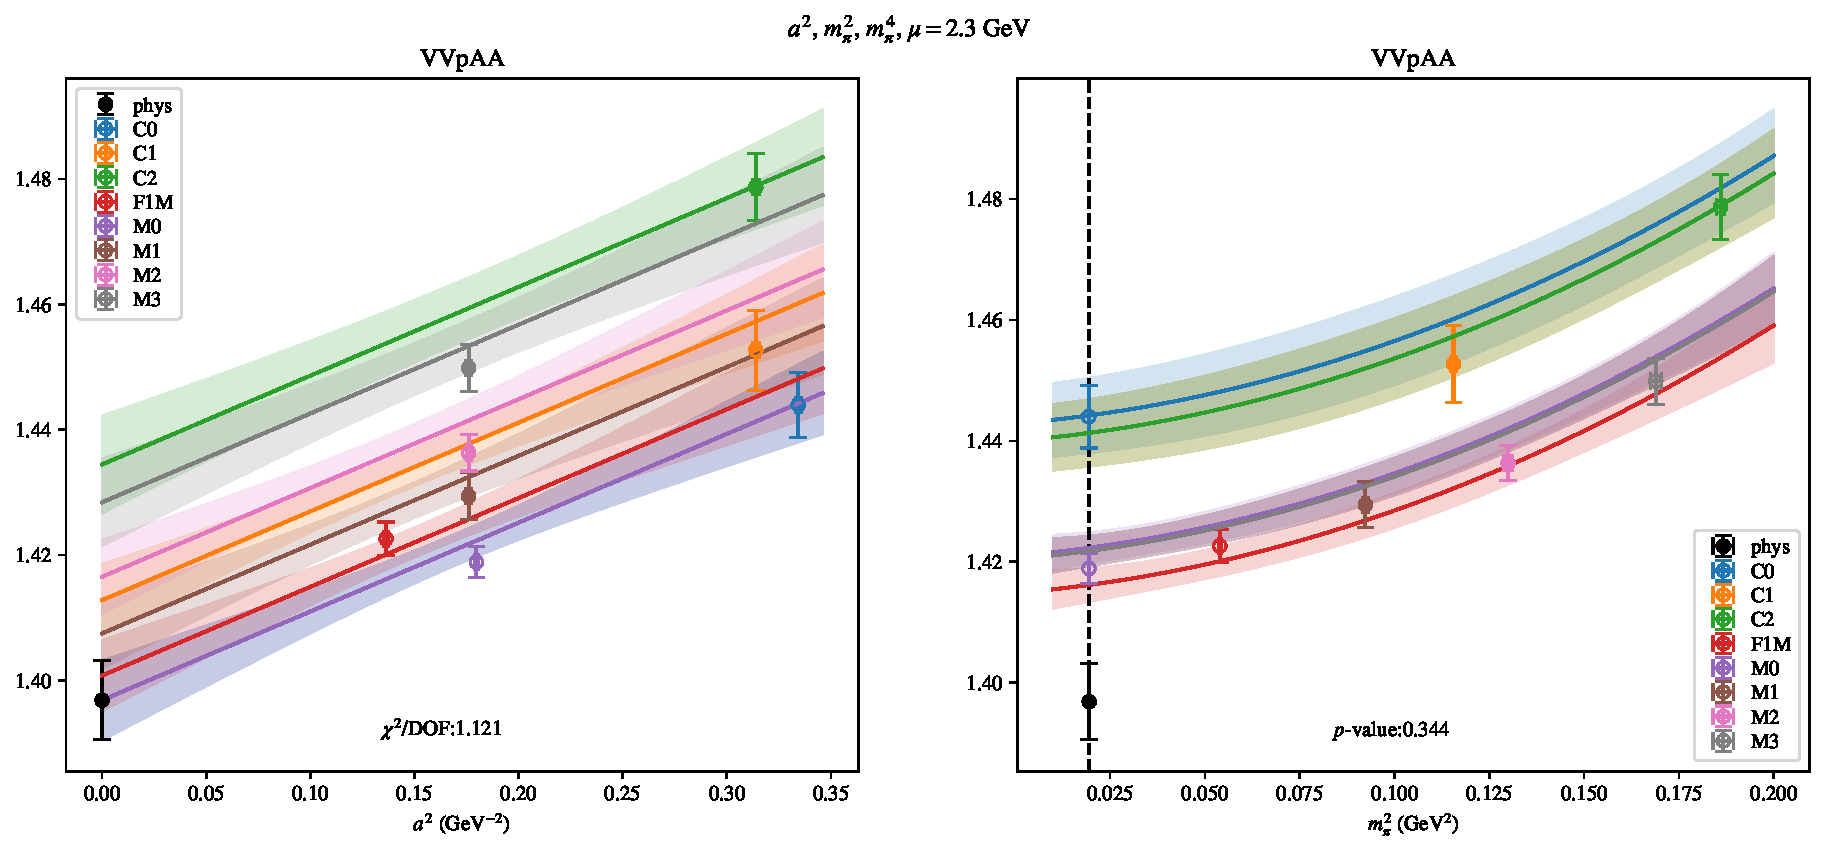
\includepdf[link, pages=-]{VVpAA/NPR/a2m2m4_23.pdf}
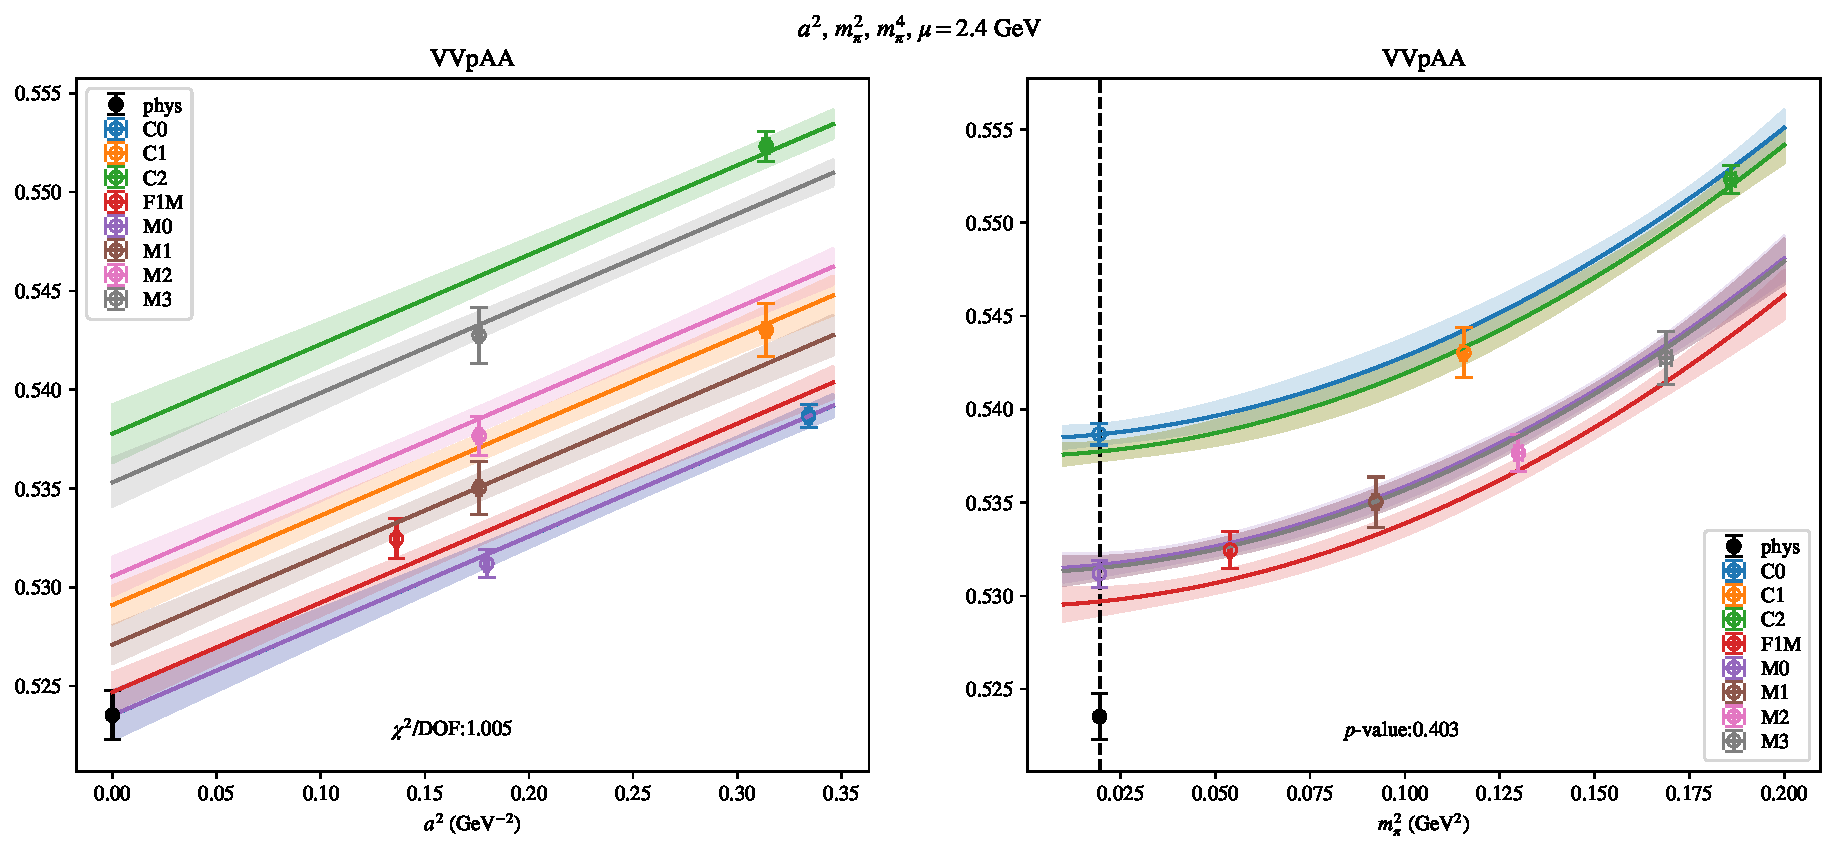
\includepdf[link, pages=-]{VVpAA/NPR/a2m2m4_24.pdf}
\clearpage
\section{$\mathcal{B}_2$}
\begin{table}[h!]
\begin{center}
\begin{tabular}{|c|c|c|c|c|c|}
\hline
$\mu$ (GeV) & $a^2$, $m_\pi^2$& $a^2$, $m_\pi^2$ (no C)& $a^2$, $a^4$, $m_\pi^2$& $a^2$, $m_\pi^2$ (no M3, C2)& $a^2$, $m_\pi^2$, $m_\pi^4$\\
\hline
2.0& \hyperlink{VVmAA/NPR/a2m2_20.pdf.1}{\textbf{-1.015(19)}: 3.439 (0.004)} & \hyperlink{VVmAA/NPR/a2m2noC_20.pdf.1}{\textbf{-0.98(11)}: 3.537 (0.029)} & \hyperlink{VVmAA/NPR/a2a4m2_20.pdf.1}{\textbf{-0.97(19)}: 3.143 (0.014)} & \hyperlink{VVmAA/NPR/a2m2mcut_20.pdf.1}{\textbf{-1.014(19)}: 4.619 (0.003)} & \hyperlink{VVmAA/NPR/a2m2m4_20.pdf.1}{\textbf{-1.016(19)}: 3.512 (0.007)}\\
2.2& \hyperlink{VVmAA/NPR/a2m2_22.pdf.1}{\textbf{-1.019(17)}: 4.451 (0.0)} & \hyperlink{VVmAA/NPR/a2m2noC_22.pdf.1}{\textbf{-0.987(85)}: 3.848 (0.021)} & \hyperlink{VVmAA/NPR/a2a4m2_22.pdf.1}{\textbf{-0.96(13)}: 2.256 (0.061)} & \hyperlink{VVmAA/NPR/a2m2mcut_22.pdf.1}{\textbf{-1.019(17)}: 5.775 (0.001)} & \hyperlink{VVmAA/NPR/a2m2m4_22.pdf.1}{\textbf{-1.021(18)}: 3.268 (0.011)}\\
2.3& \hyperlink{VVmAA/NPR/a2m2_23.pdf.1}{\textbf{-1.022(18)}: 4.65 (0.0)} & \hyperlink{VVmAA/NPR/a2m2noC_23.pdf.1}{\textbf{-0.988(88)}: 3.788 (0.023)} & \hyperlink{VVmAA/NPR/a2a4m2_23.pdf.1}{\textbf{-0.96(14)}: 2.259 (0.06)} & \hyperlink{VVmAA/NPR/a2m2mcut_23.pdf.1}{\textbf{-1.023(18)}: 6.139 (0.0)} & \hyperlink{VVmAA/NPR/a2m2m4_23.pdf.1}{\textbf{-1.024(18)}: 3.371 (0.009)}\\
2.4& \hyperlink{VVmAA/NPR/a2m2_24.pdf.1}{\textbf{-1.026(16)}: 5.04 (0.0)} & \hyperlink{VVmAA/NPR/a2m2noC_24.pdf.1}{\textbf{-0.990(90)}: 4.278 (0.014)} & \hyperlink{VVmAA/NPR/a2a4m2_24.pdf.1}{\textbf{-0.97(14)}: 2.67 (0.03)} & \hyperlink{VVmAA/NPR/a2m2mcut_24.pdf.1}{\textbf{-1.026(17)}: 6.4 (0.0)} & \hyperlink{VVmAA/NPR/a2m2m4_24.pdf.1}{\textbf{-1.028(17)}: 3.62 (0.006)}\\
\hline
\end{tabular}
\caption{Physical point value from chiral and continuum extrapolation at renormalisation scale $\mu$. Entries are \textbf{value(error)}: $\chi^2/\text{DOF}$ ($p$-value).}
\end{center}
\end{table}
\begin{table}[h!]
\begin{center}
\begin{tabular}{|c c|c|c|c|c|c|}
\hline
$\mu$ (GeV) &  & $a^2$, $m_\pi^2$& $a^2$, $m_\pi^2$ (no C)& $a^2$, $a^4$, $m_\pi^2$& $a^2$, $m_\pi^2$ (no M3, C2)& $a^2$, $m_\pi^2$, $m_\pi^4$\\
\hline
\multirow{2}{0.5in}{2.0} & $\alpha$ & -0.186(67)& 0.007& 0.16(18)& -0.184(66)& -0.189(67)\\
 & $\beta$ & 0.00194(20)& 0.00233(27)& 0.00194(21)& 0.00183(26)& 0.00032(78)\\
\hline
\multirow{2}{0.5in}{2.2} & $\alpha$ & -0.222(60)& -0.04(49)& 0.23(13)& -0.223(60)& -0.228(62)\\
 & $\beta$ & 0.00168(18)& 0.00177(23)& 0.00164(20)& 0.00132(26)& -0.0005(73)\\
\hline
\multirow{2}{0.5in}{2.3} & $\alpha$ & -0.245(62)& -0.05(50)& 0.22(13)& -0.246(62)& -0.251(64)\\
 & $\beta$ & 0.00156(18)& 0.00165(22)& 0.00152(19)& 0.00121(25)& -0.0007(74)\\
\hline
\multirow{2}{0.5in}{2.4} & $\alpha$ & -0.267(60)& -0.06(51)& 0.20(13)& -0.268(61)& -0.273(62)\\
 & $\beta$ & 0.00146(16)& 0.00158(21)& 0.00143(17)& 0.00109(23)& -0.0008(71)\\
\hline
\end{tabular}
\caption{Fit values of coefficients in $Q = Q_{phys} + \mathbf{\alpha} a^2 + \mathbf{\beta}\left(\frac{m_\pi^2}{f_\pi^2}-\frac{m_{\pi,PDG}^2}{f_\pi^2}\right) + \ldots$.}
\end{center}
\end{table}
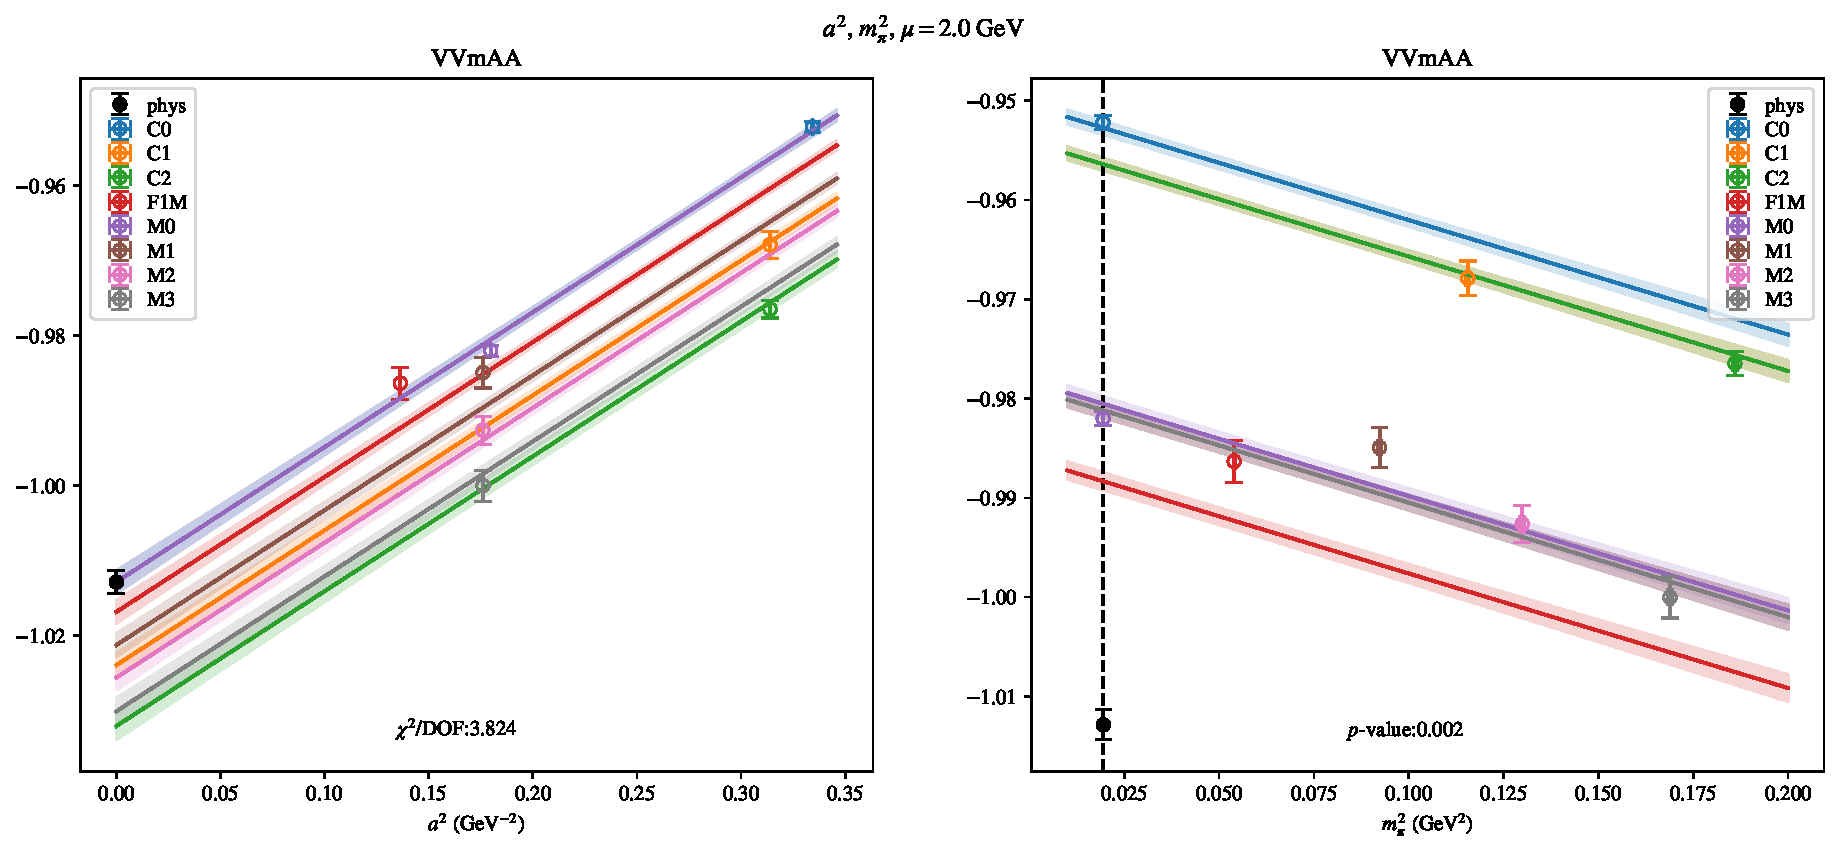
\includepdf[link, pages=-]{VVmAA/NPR/a2m2_20.pdf}
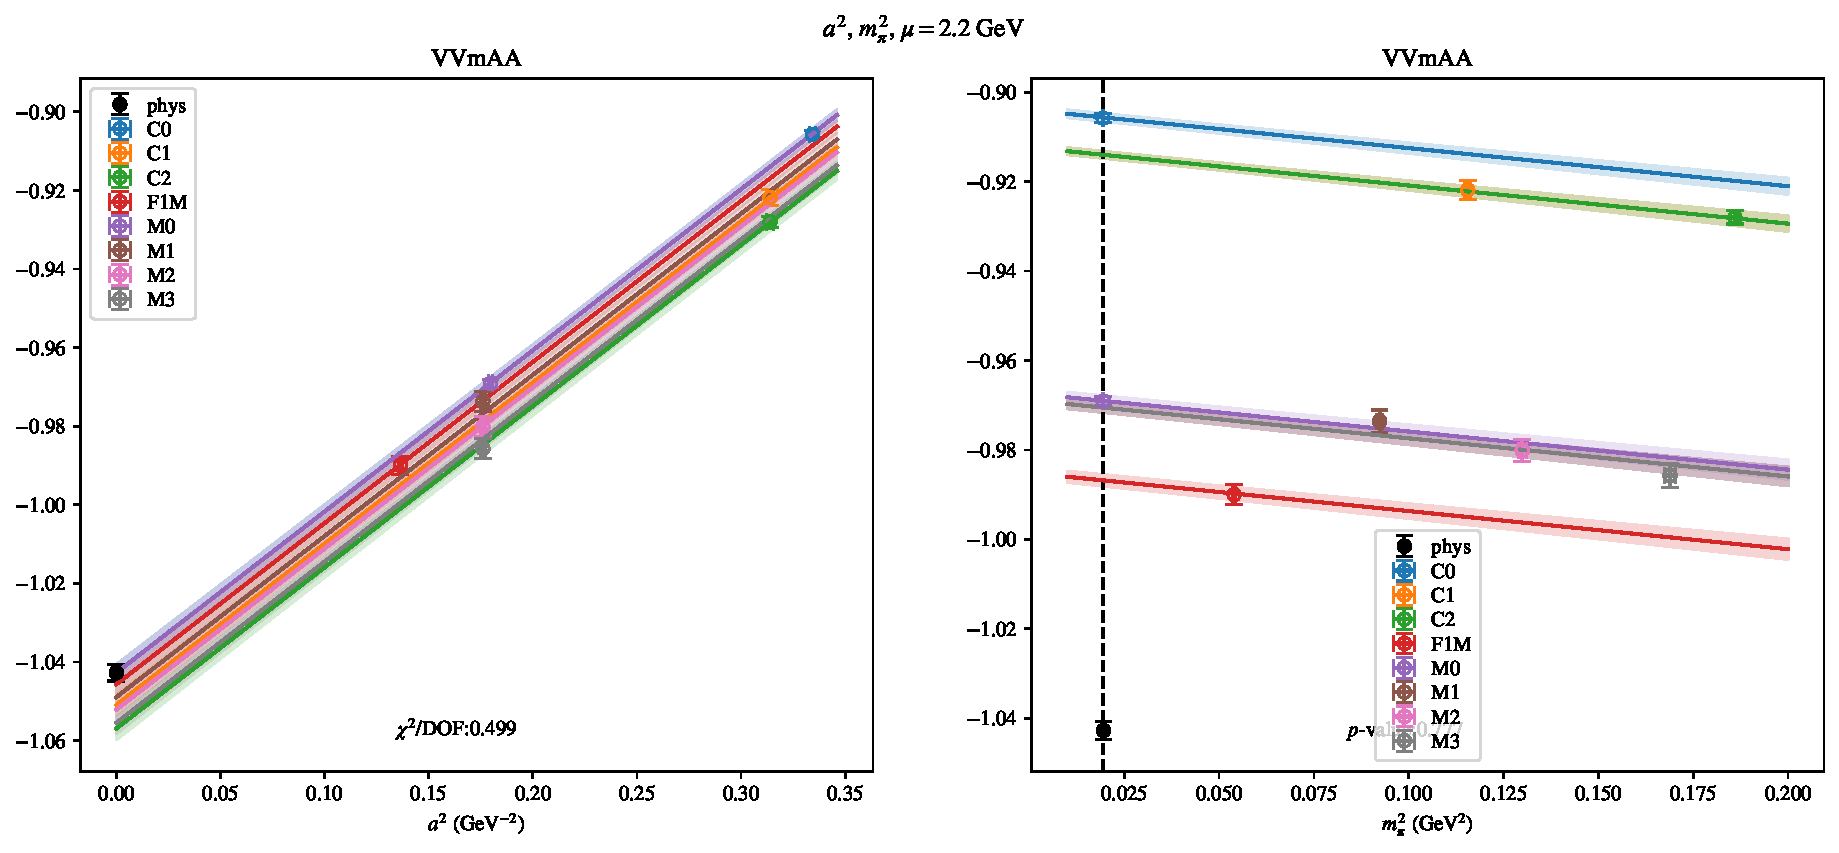
\includepdf[link, pages=-]{VVmAA/NPR/a2m2_22.pdf}
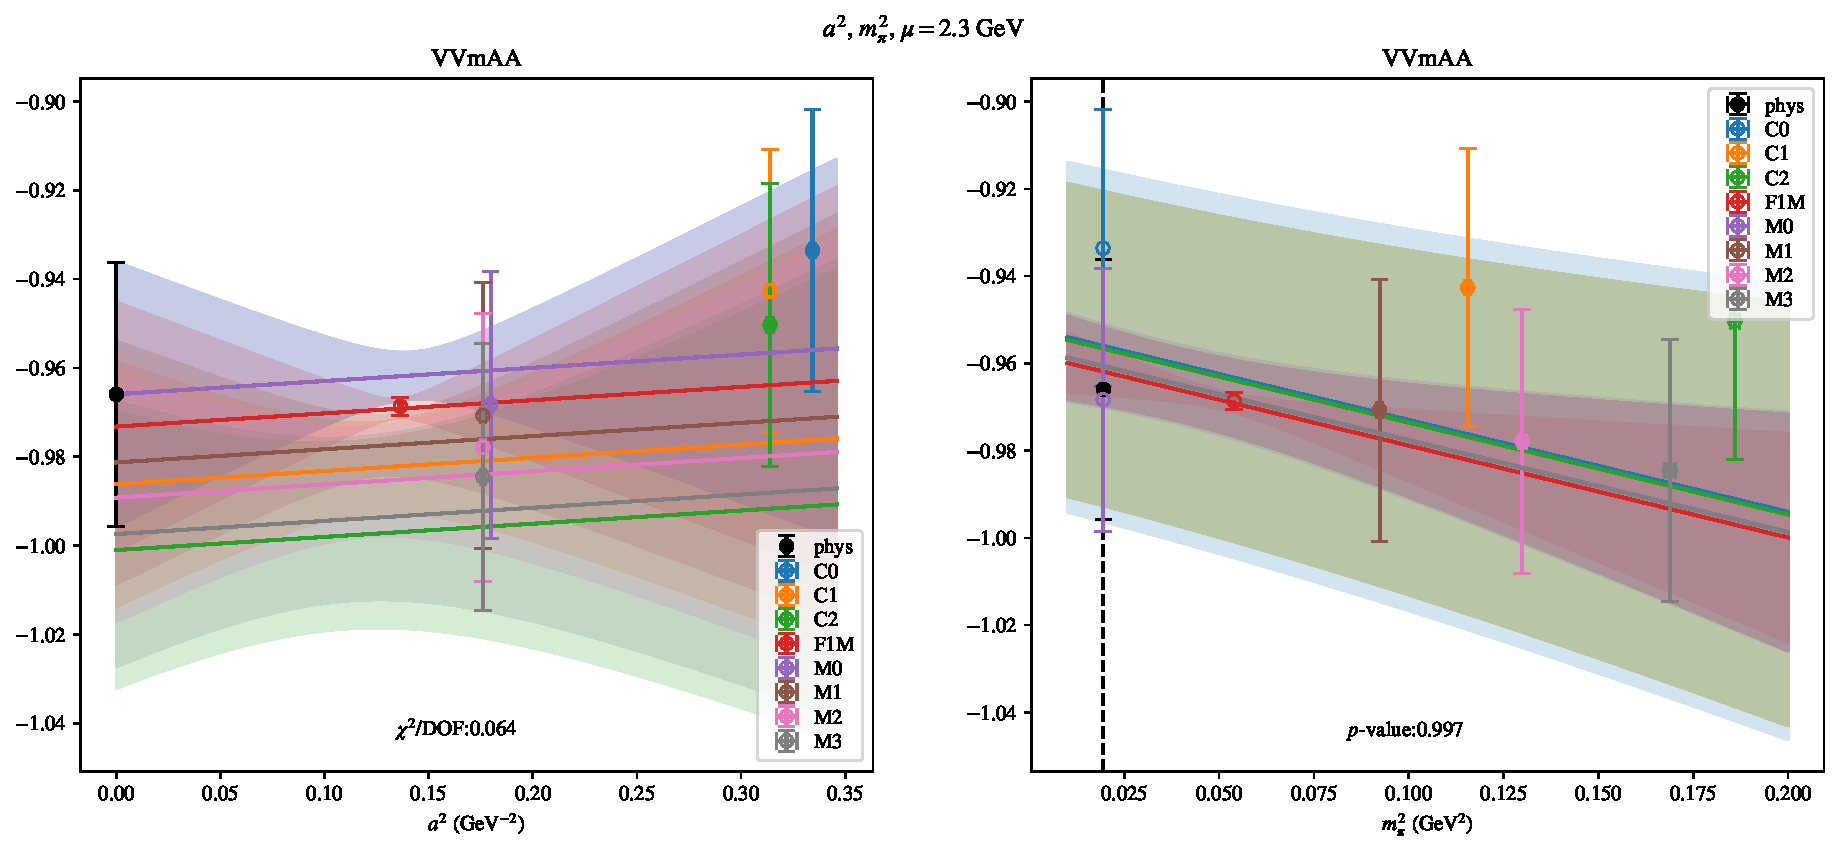
\includepdf[link, pages=-]{VVmAA/NPR/a2m2_23.pdf}
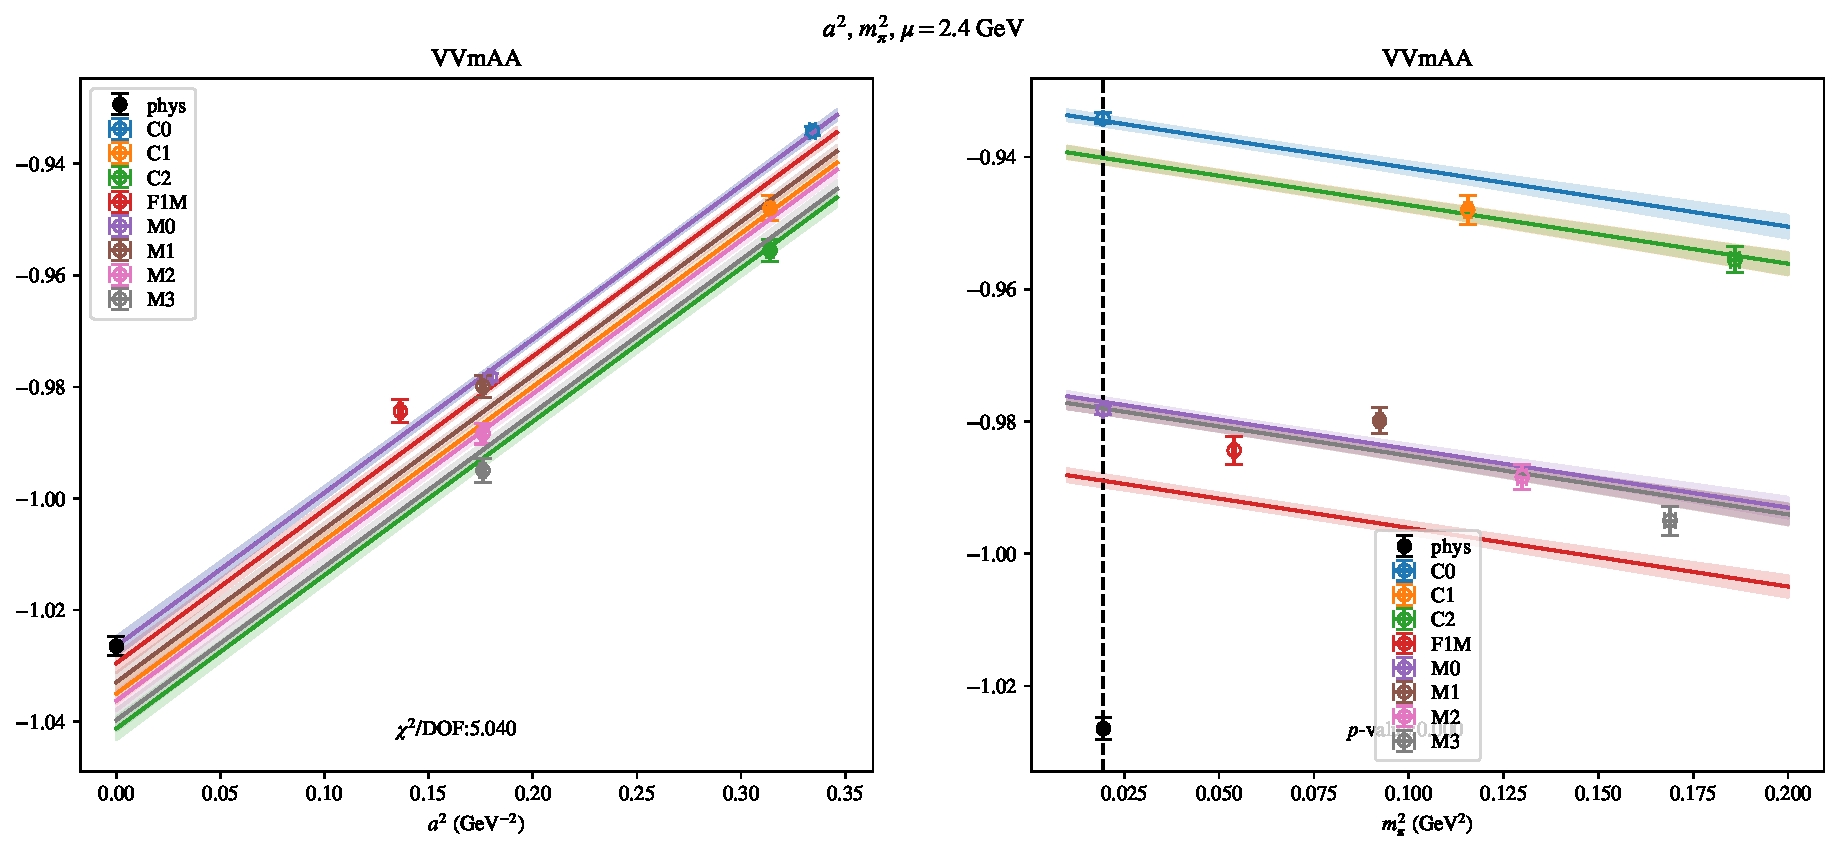
\includepdf[link, pages=-]{VVmAA/NPR/a2m2_24.pdf}
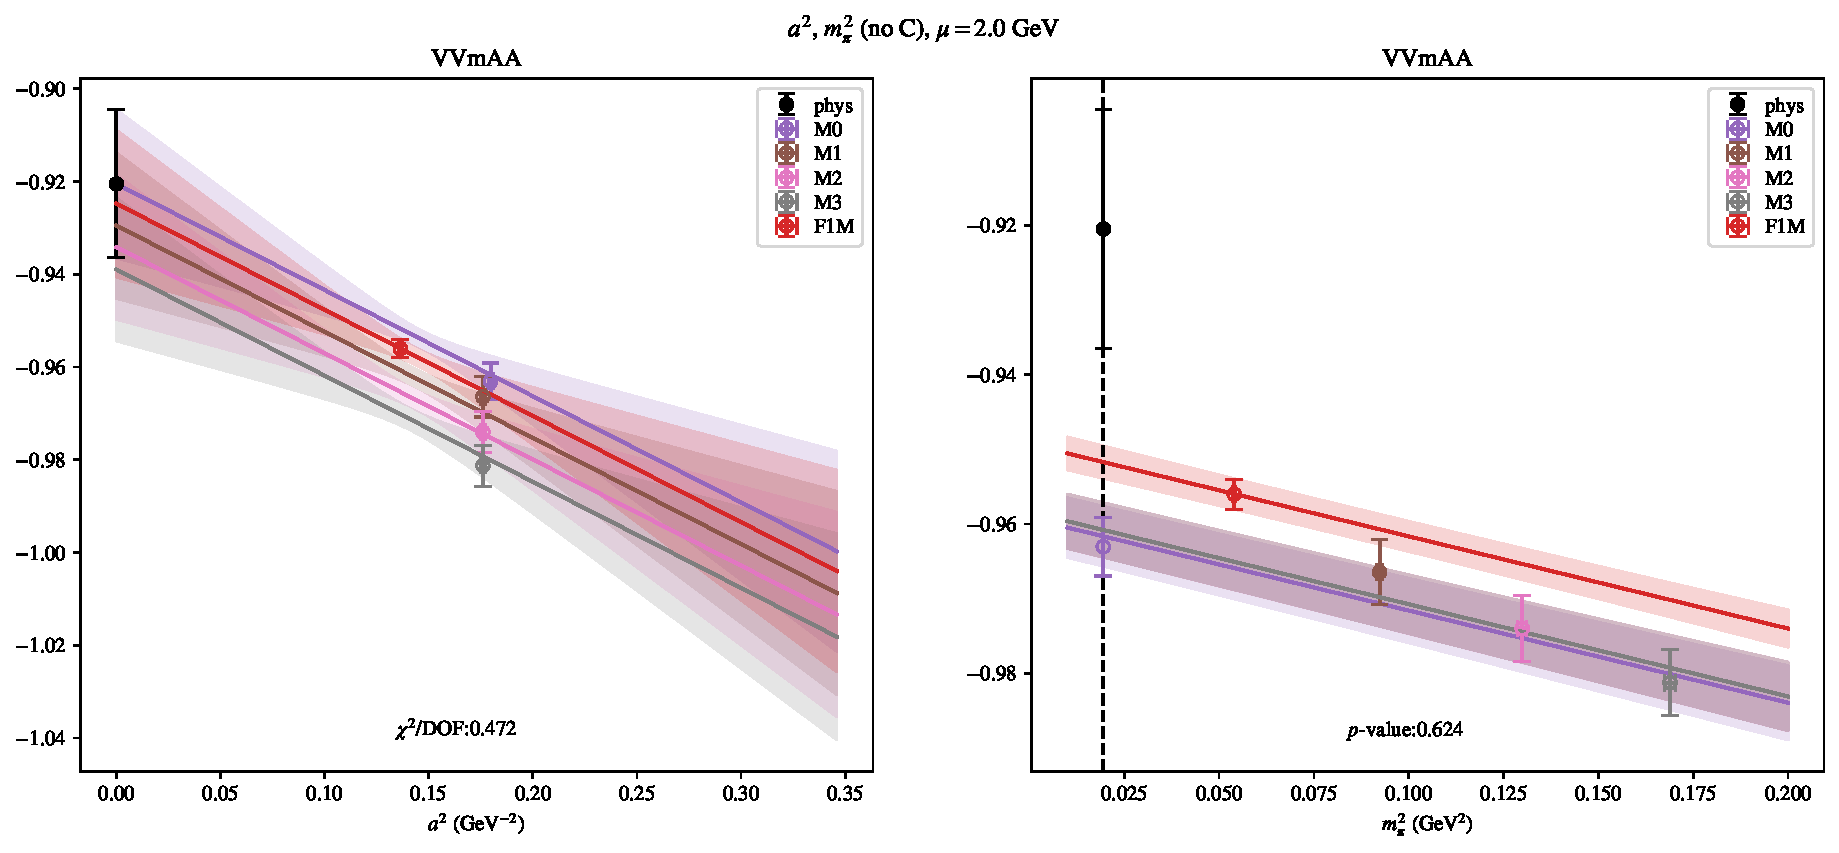
\includepdf[link, pages=-]{VVmAA/NPR/a2m2noC_20.pdf}
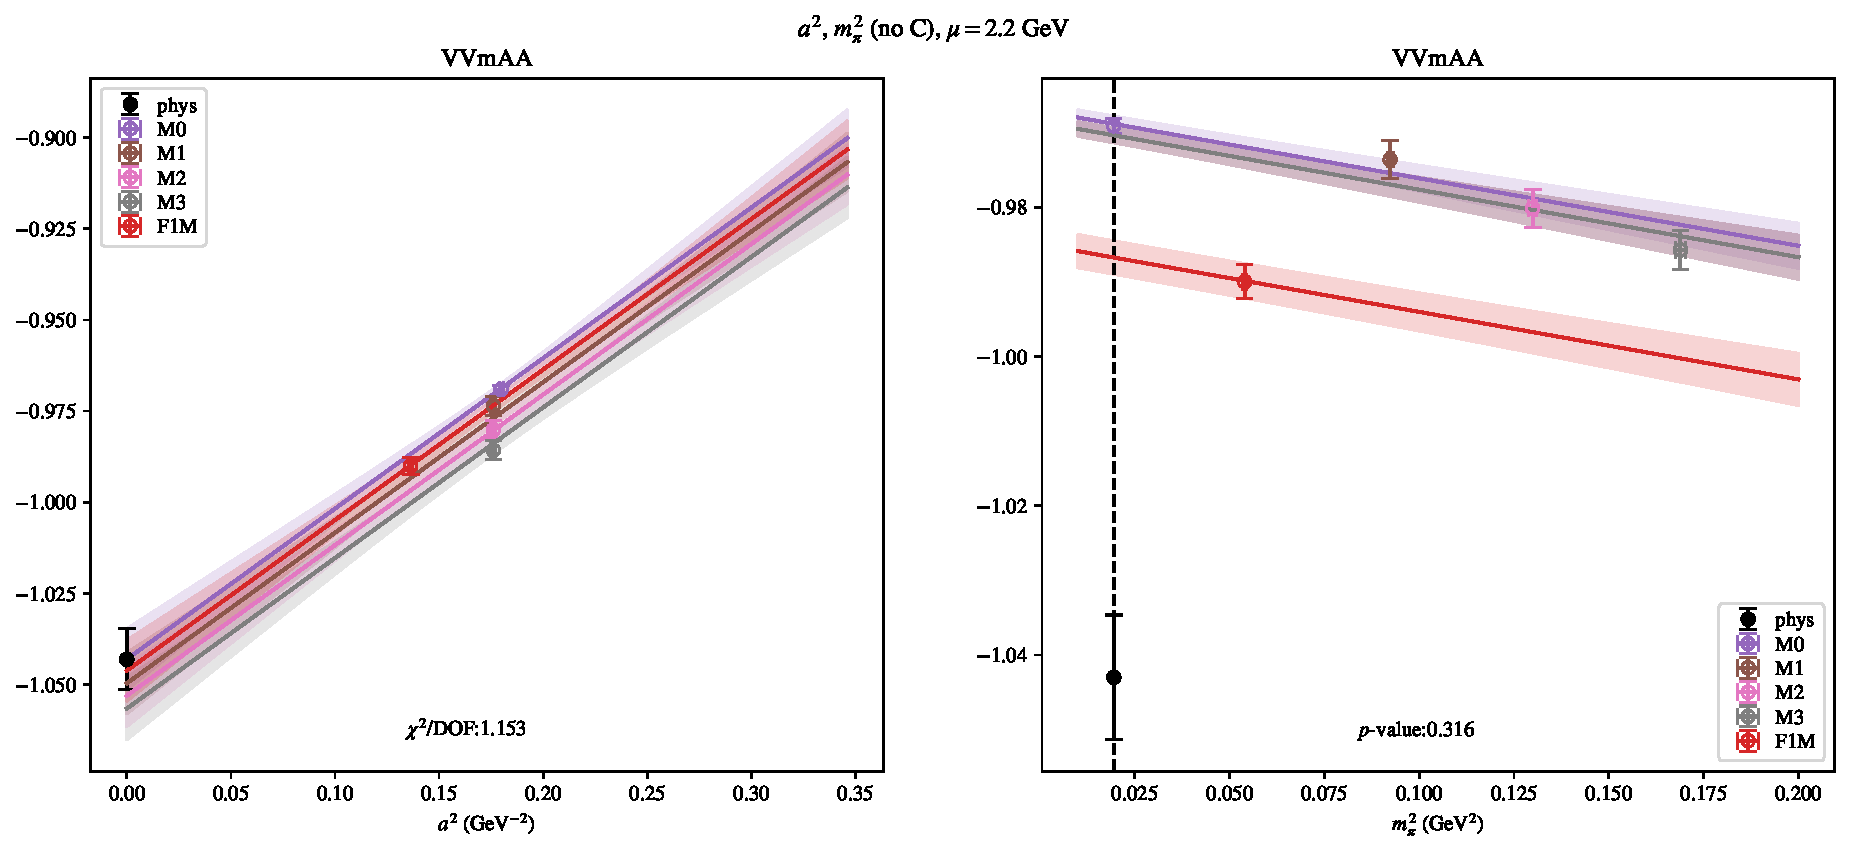
\includepdf[link, pages=-]{VVmAA/NPR/a2m2noC_22.pdf}
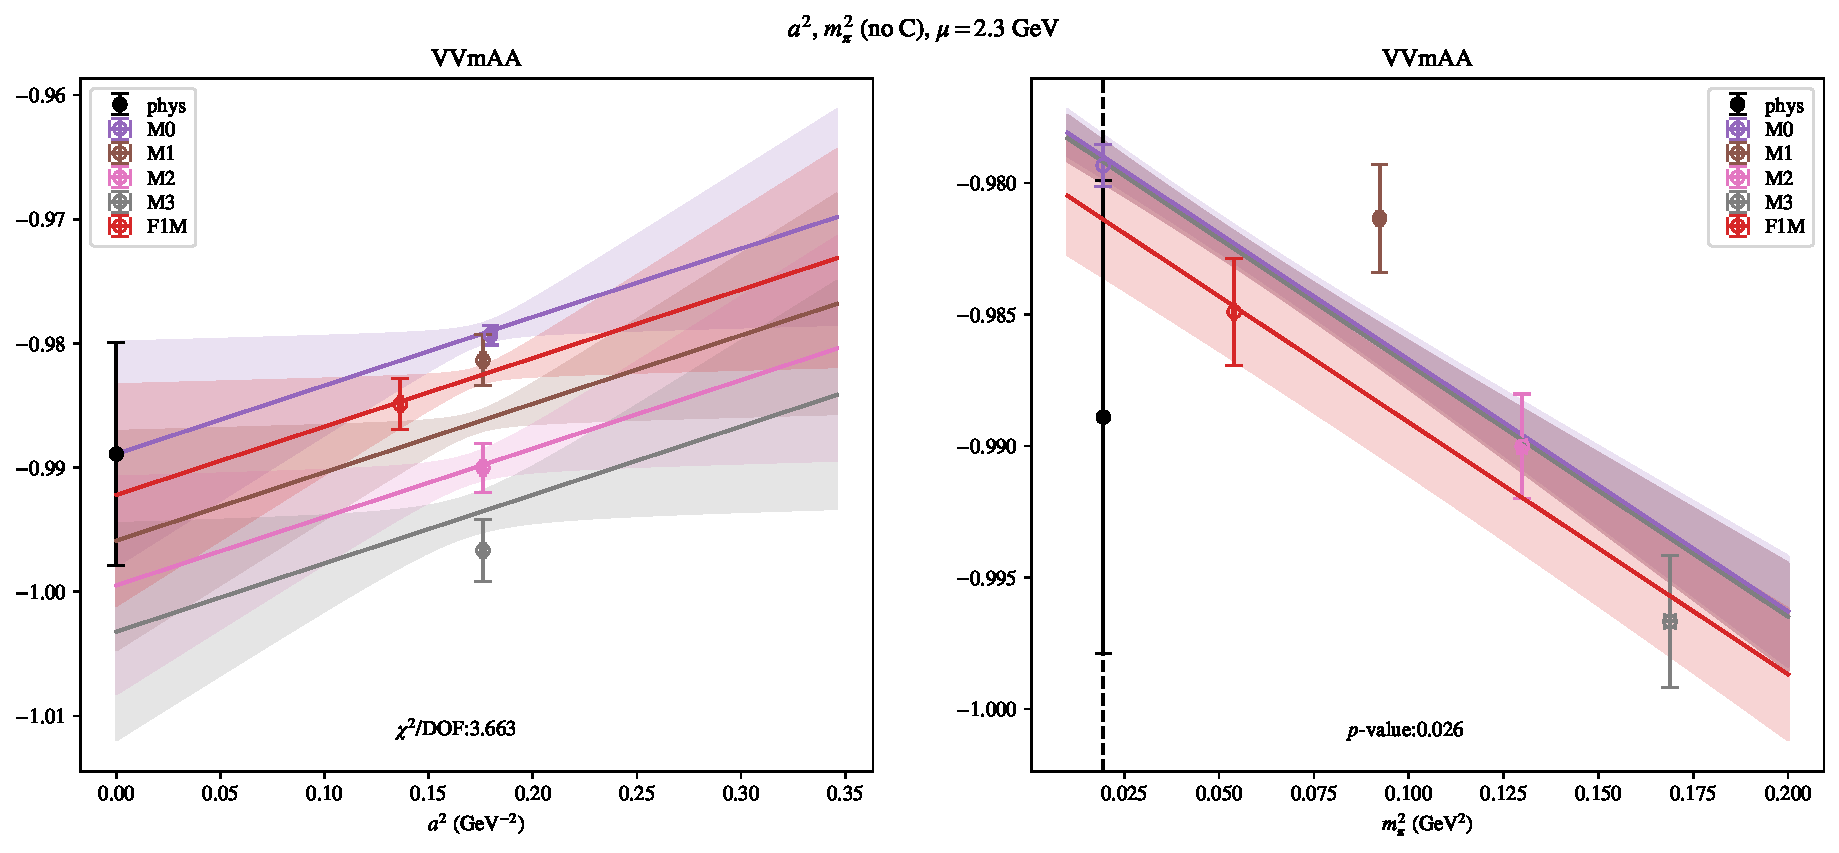
\includepdf[link, pages=-]{VVmAA/NPR/a2m2noC_23.pdf}
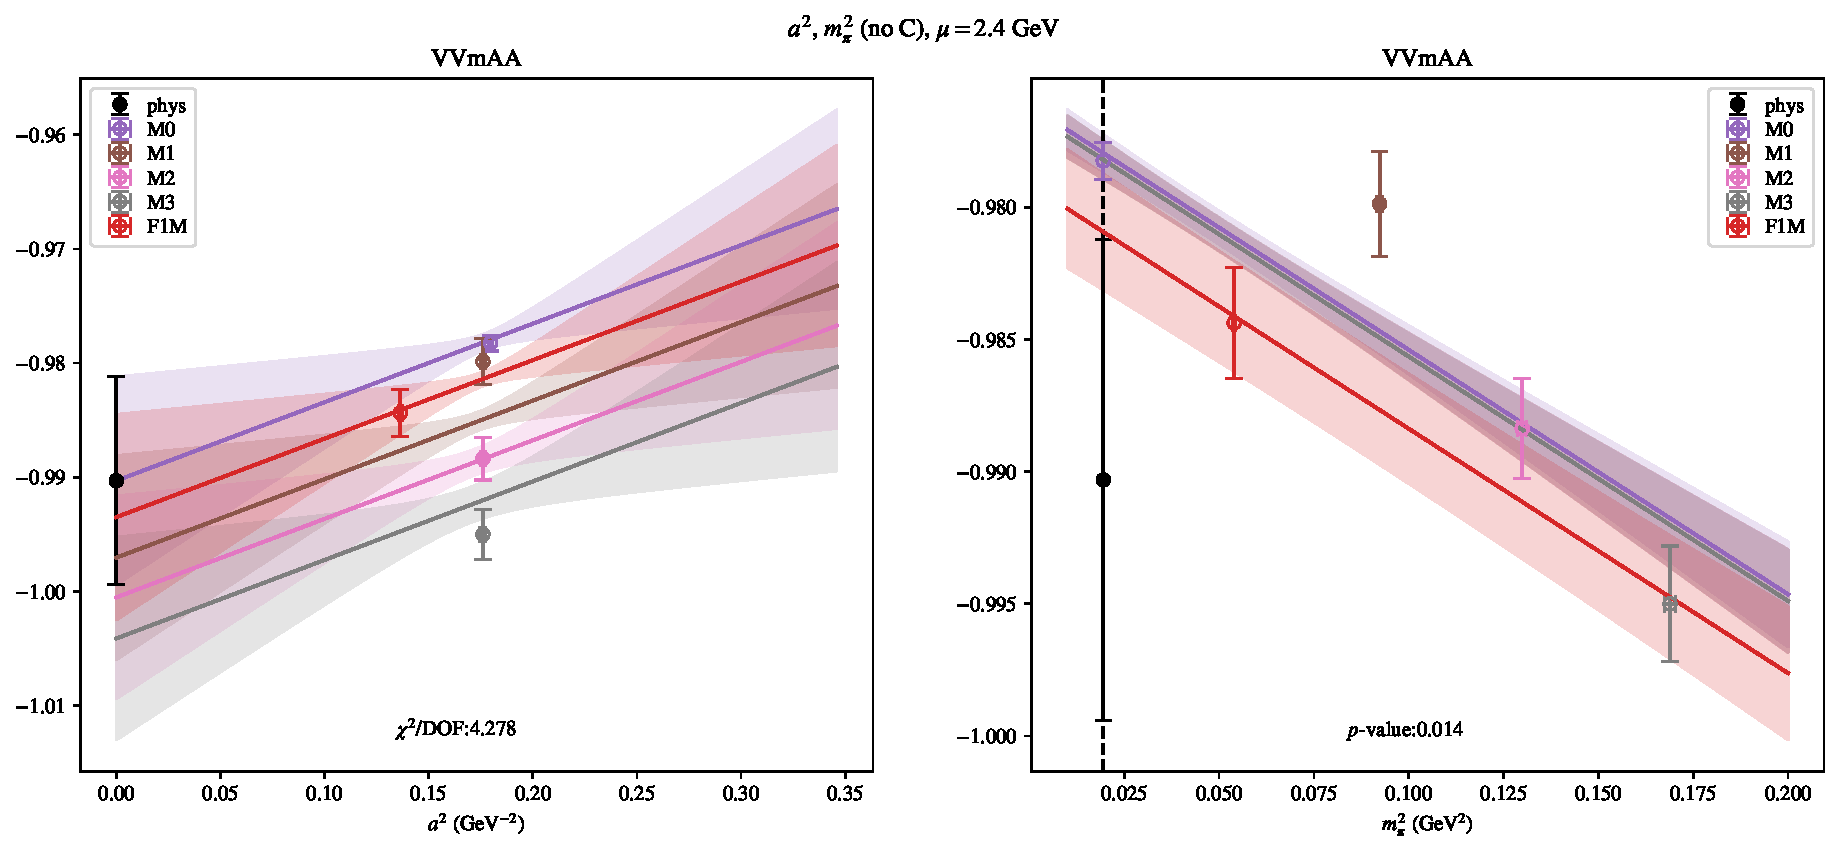
\includepdf[link, pages=-]{VVmAA/NPR/a2m2noC_24.pdf}
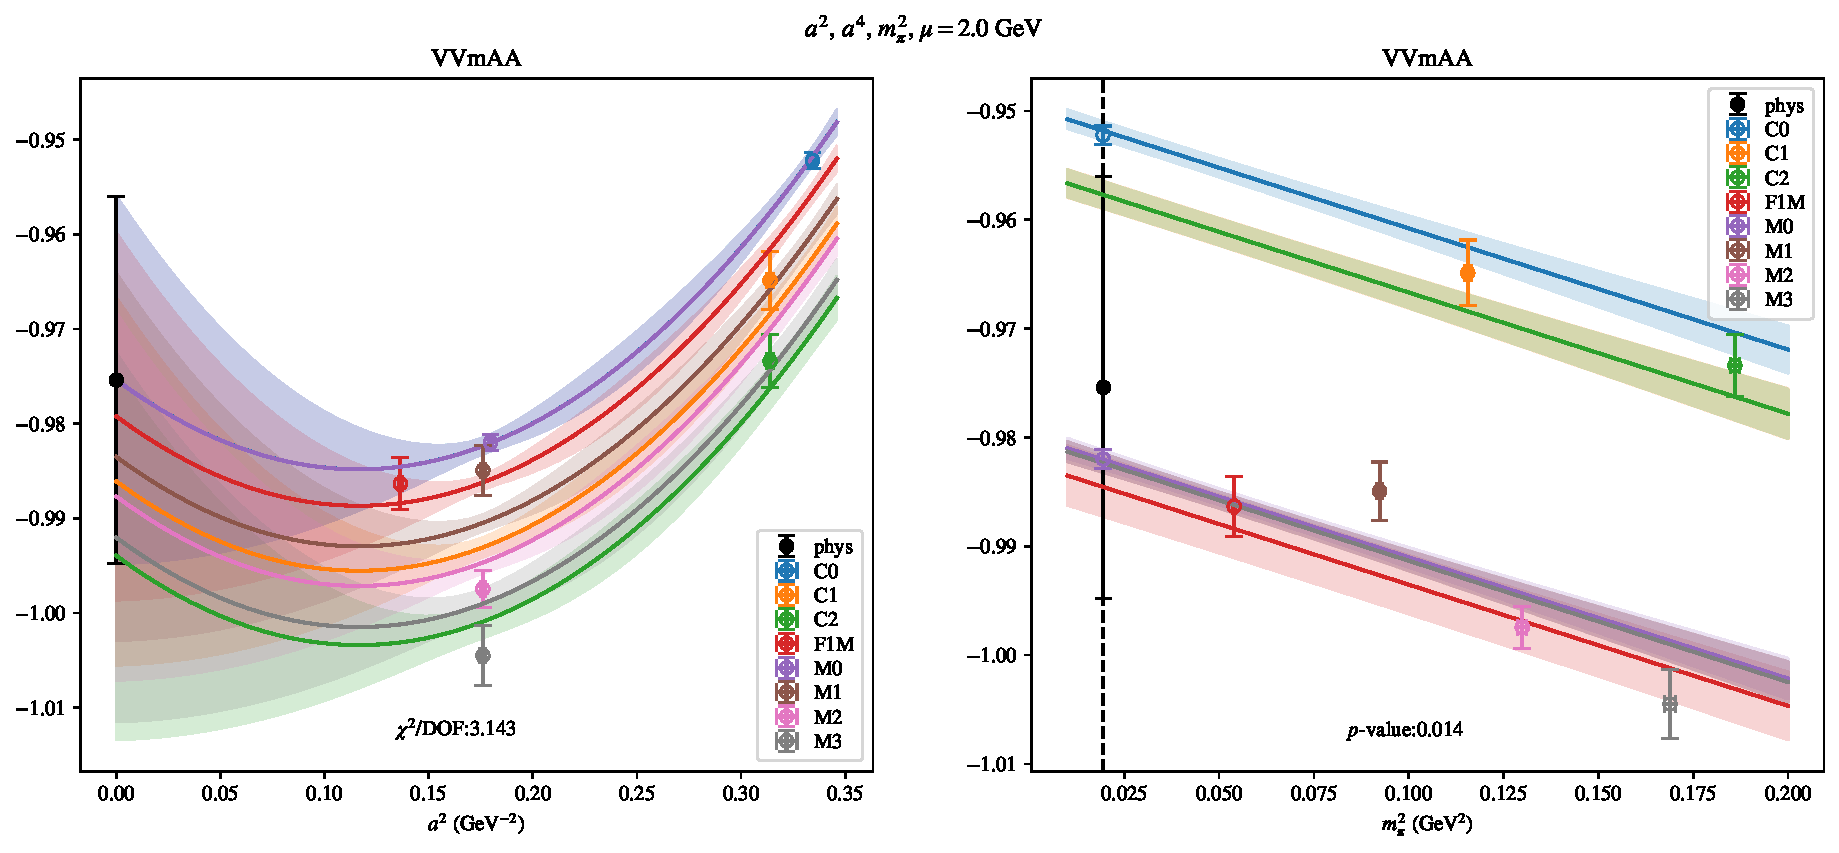
\includepdf[link, pages=-]{VVmAA/NPR/a2a4m2_20.pdf}
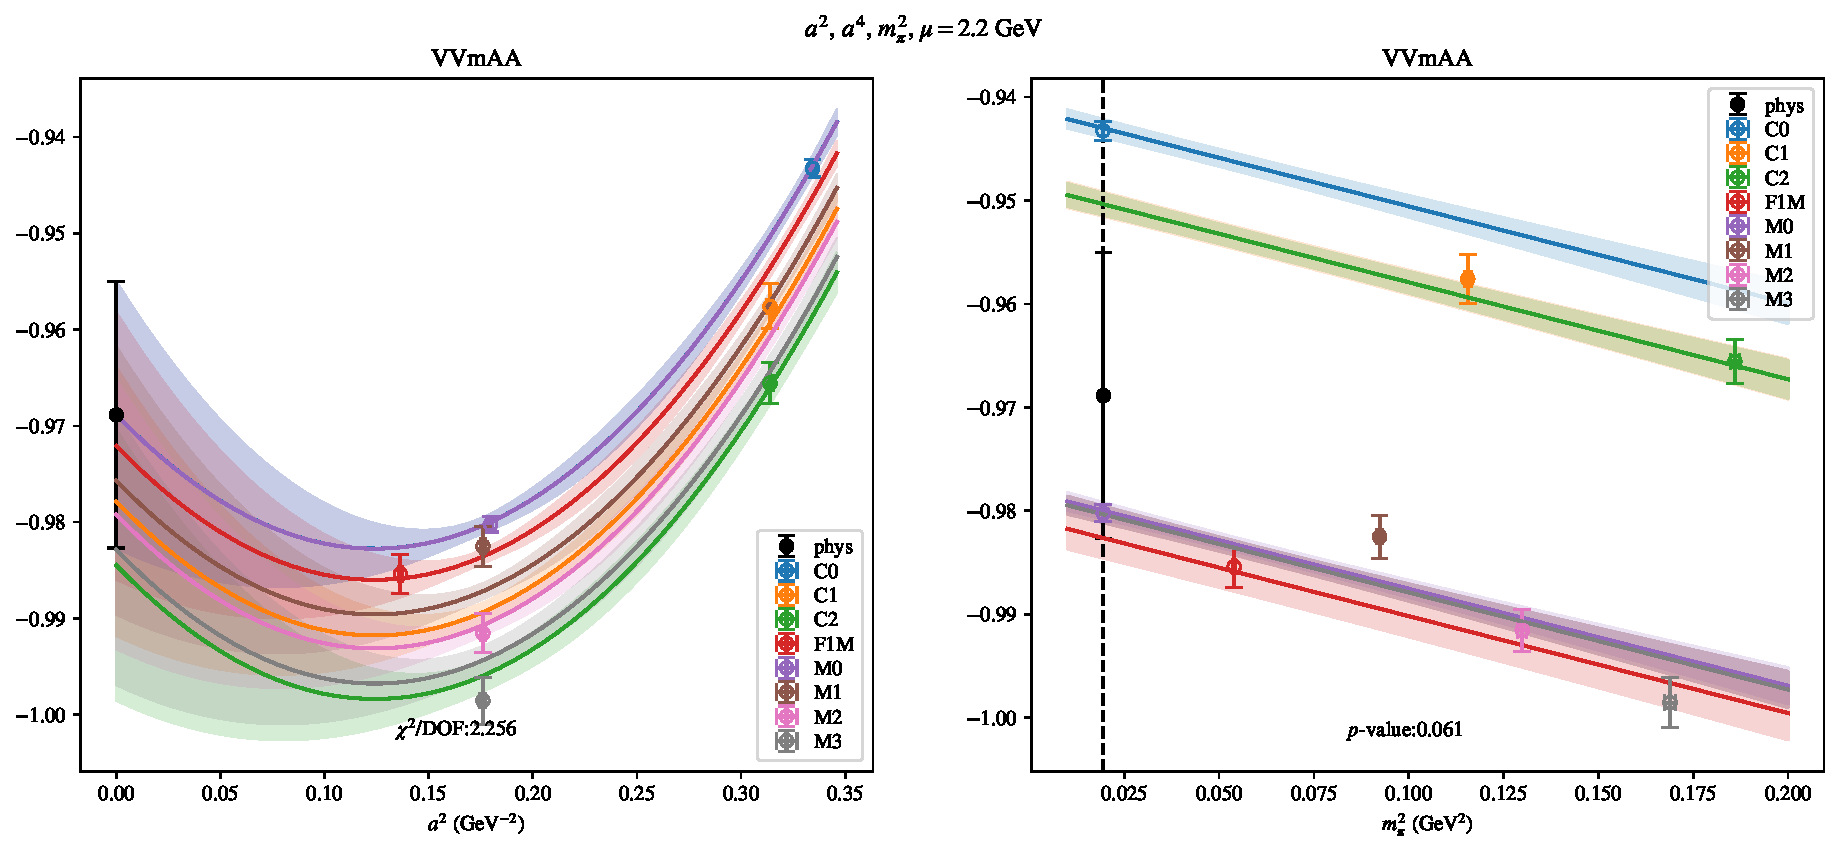
\includepdf[link, pages=-]{VVmAA/NPR/a2a4m2_22.pdf}
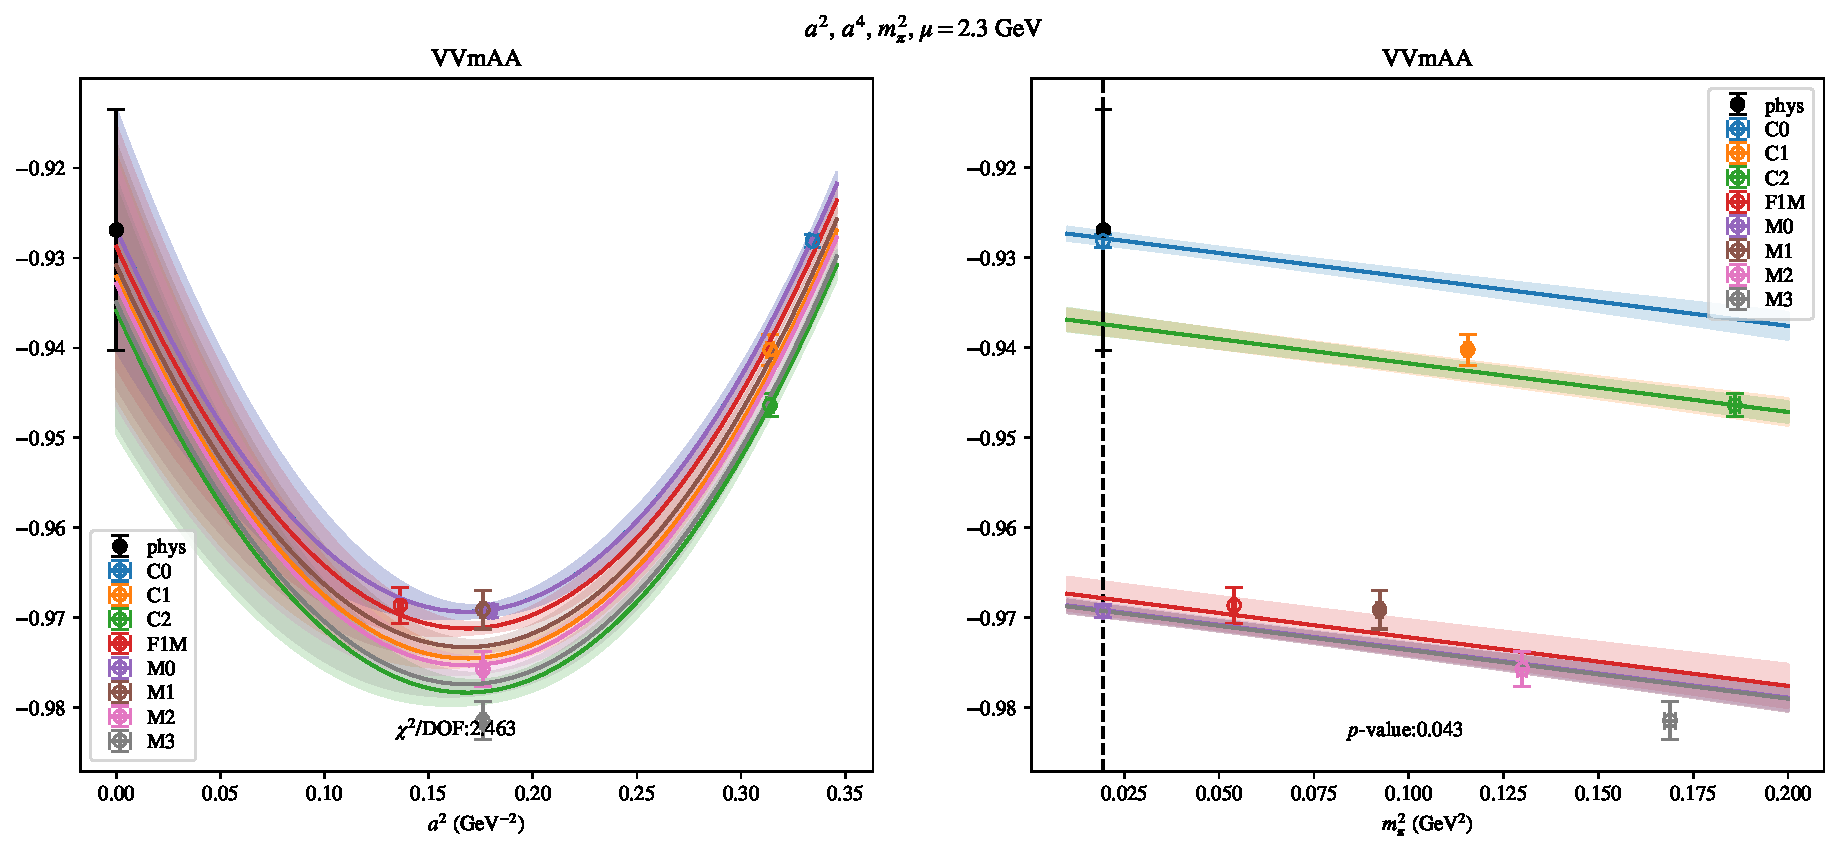
\includepdf[link, pages=-]{VVmAA/NPR/a2a4m2_23.pdf}
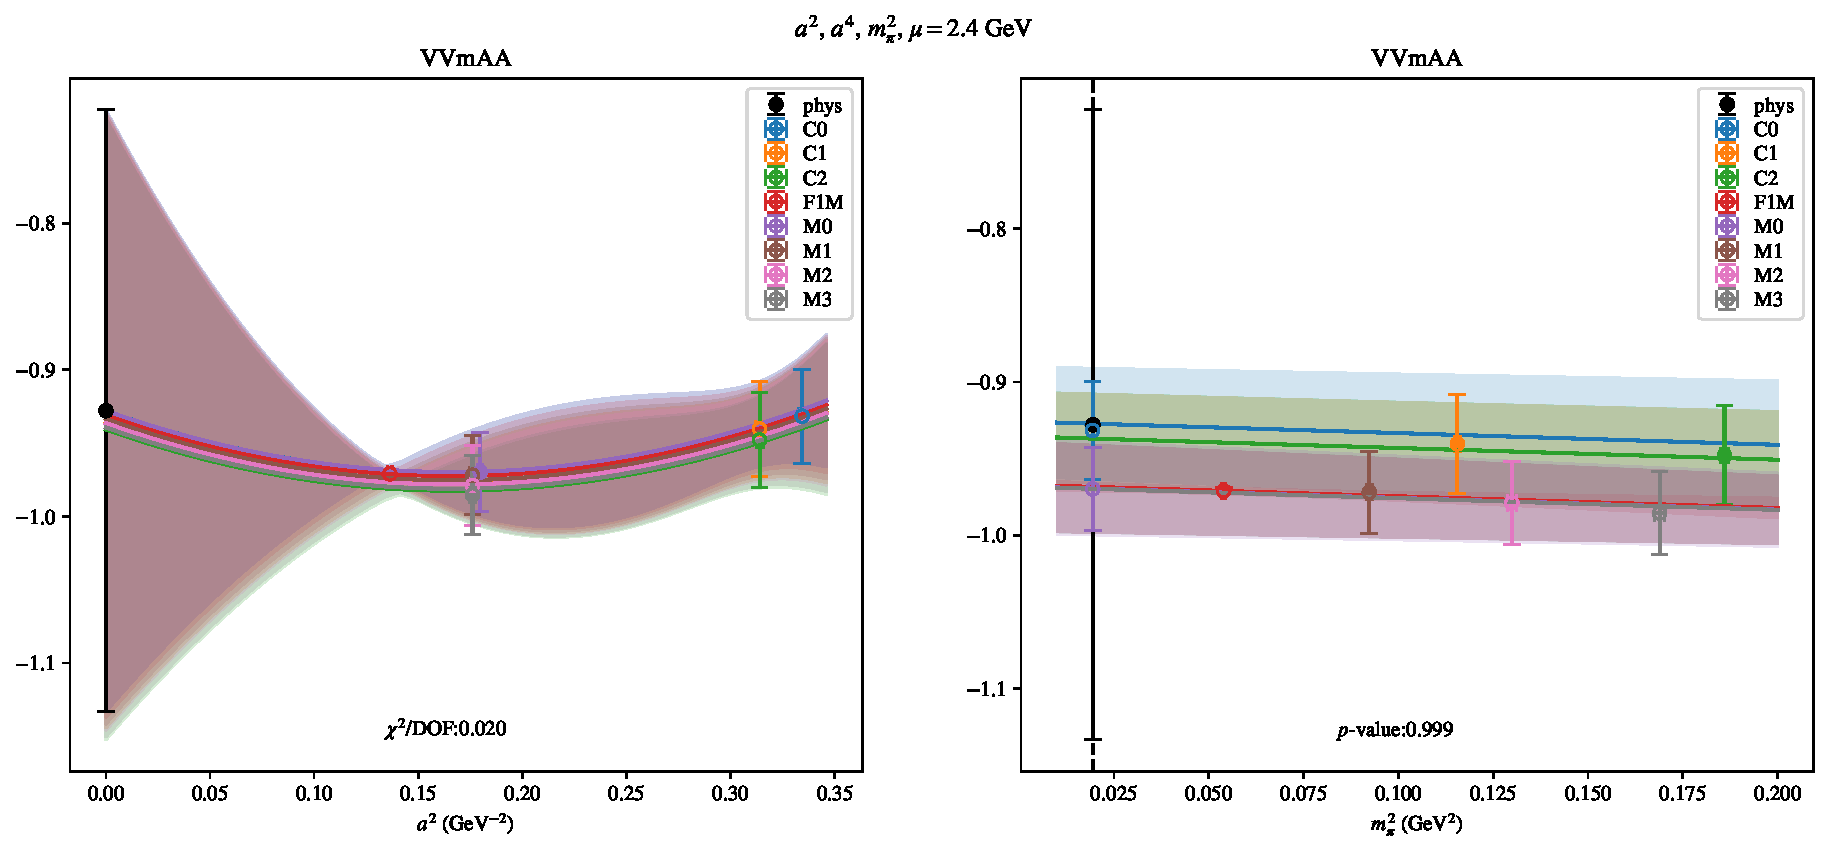
\includepdf[link, pages=-]{VVmAA/NPR/a2a4m2_24.pdf}
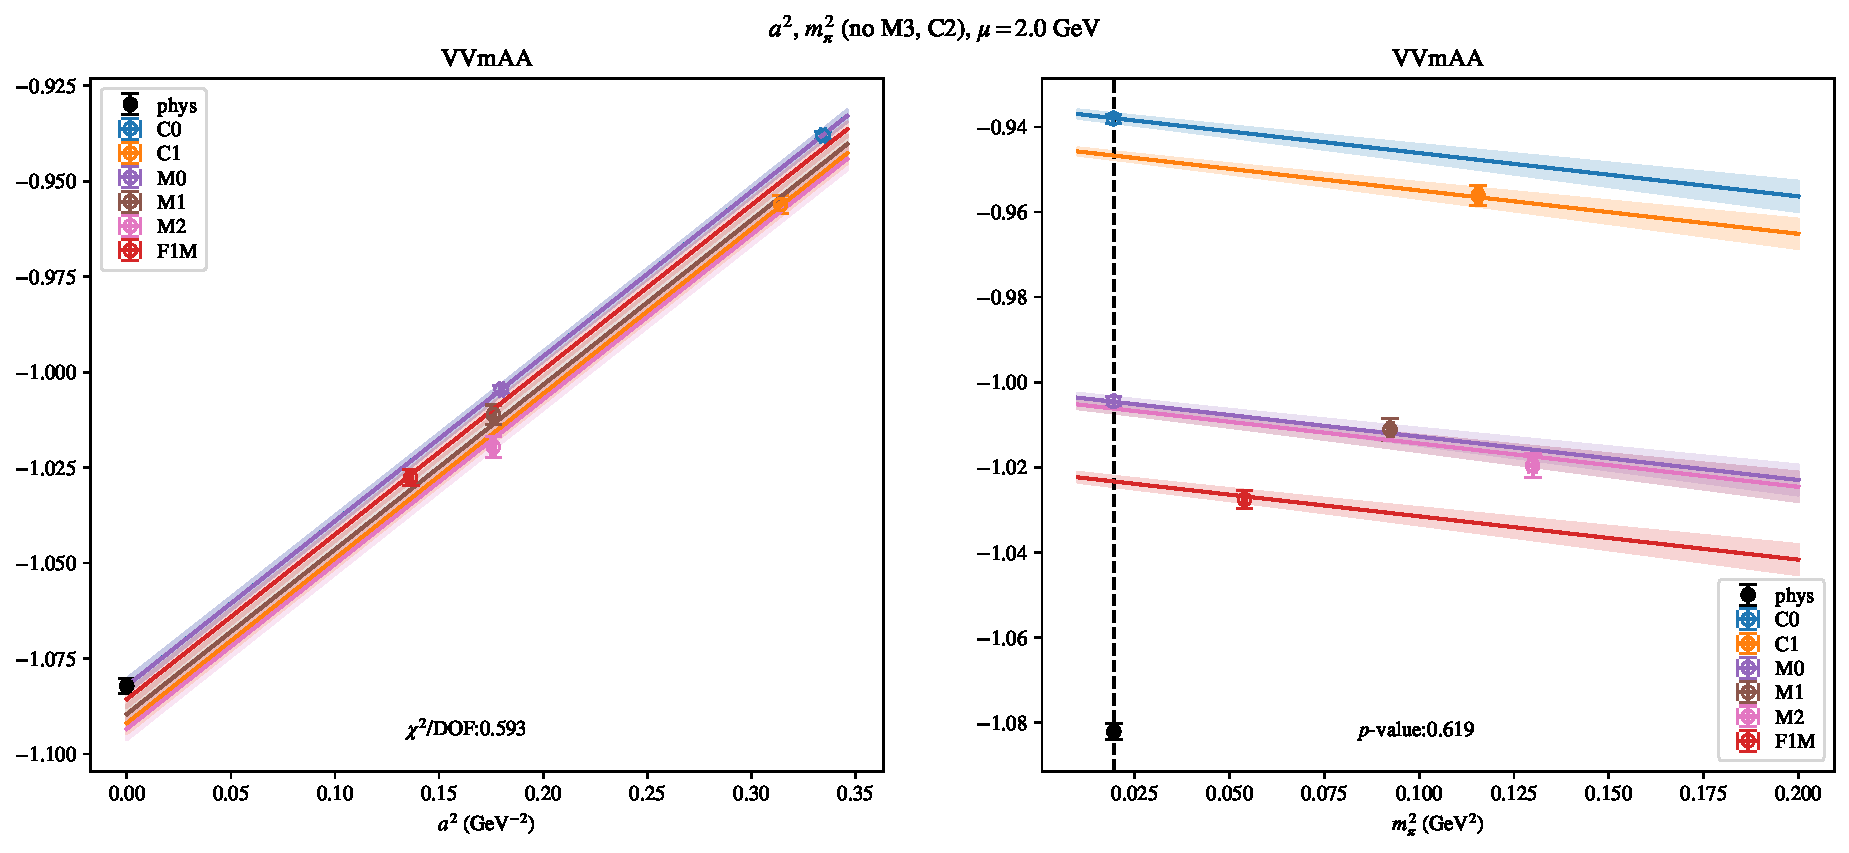
\includepdf[link, pages=-]{VVmAA/NPR/a2m2mcut_20.pdf}
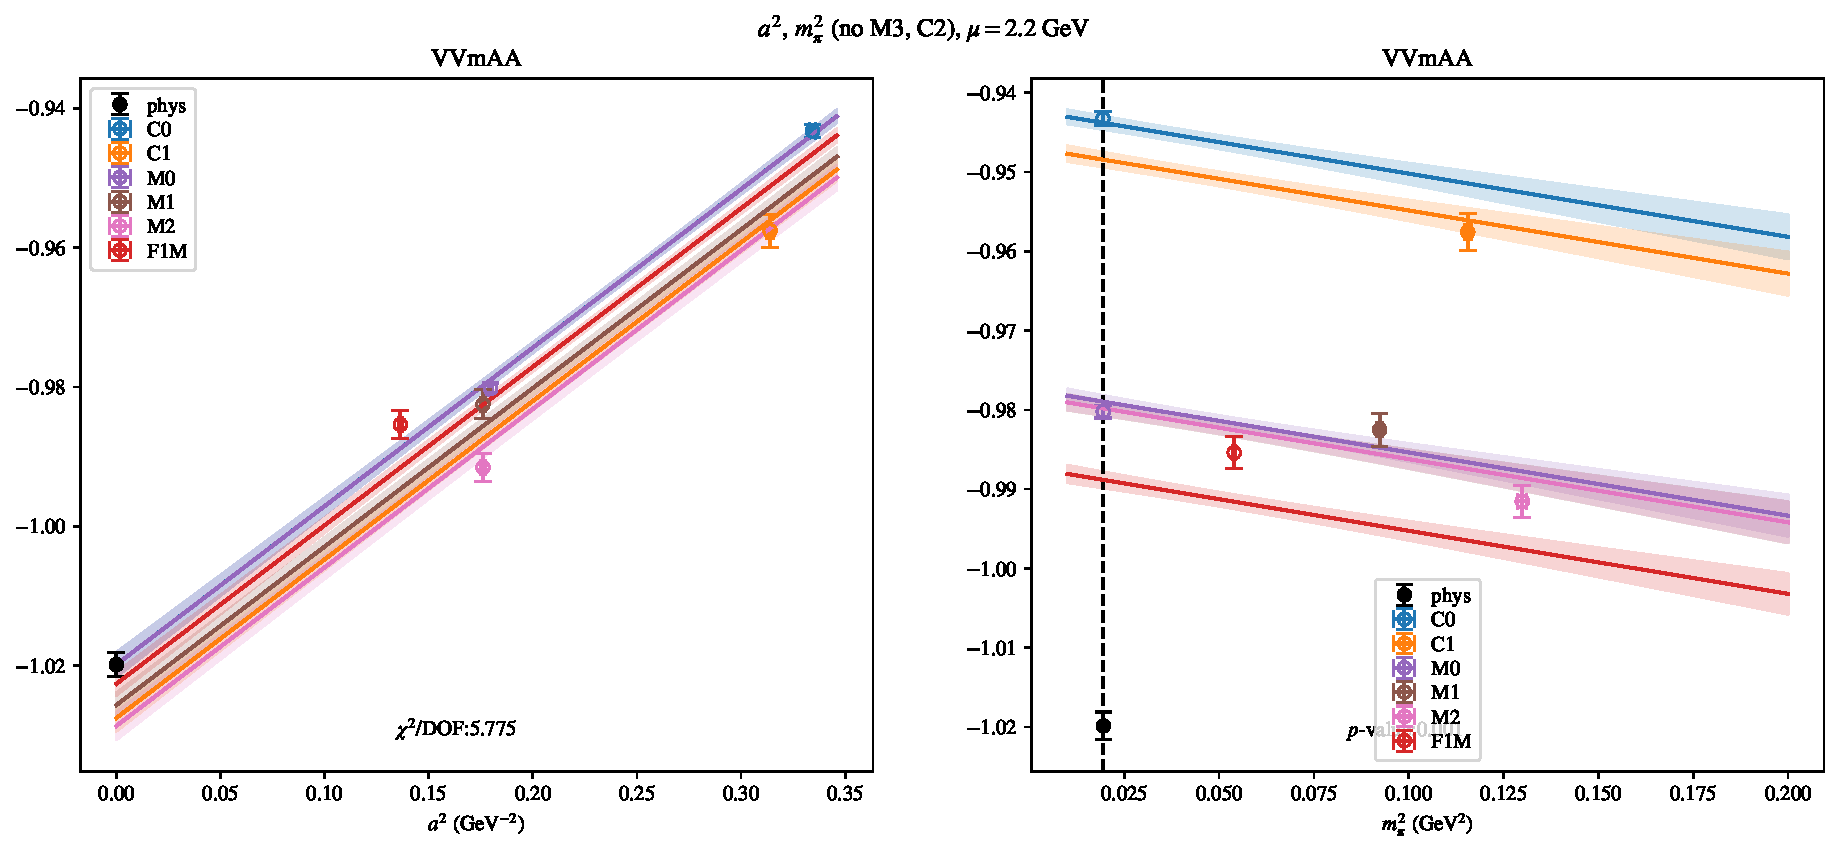
\includepdf[link, pages=-]{VVmAA/NPR/a2m2mcut_22.pdf}
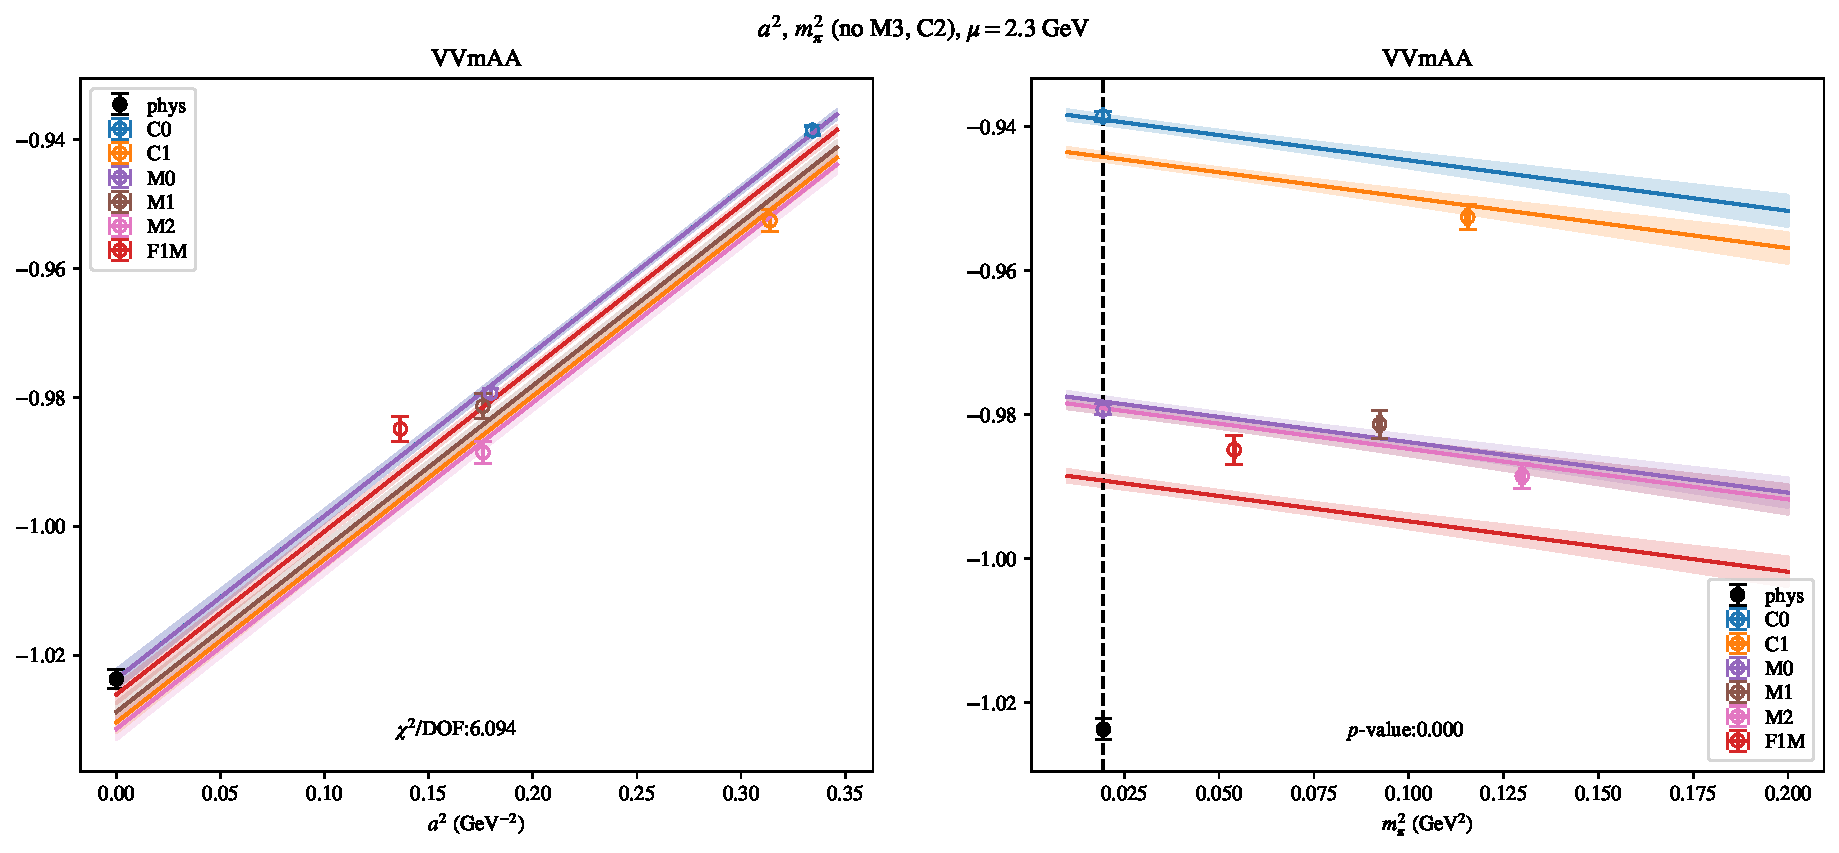
\includepdf[link, pages=-]{VVmAA/NPR/a2m2mcut_23.pdf}
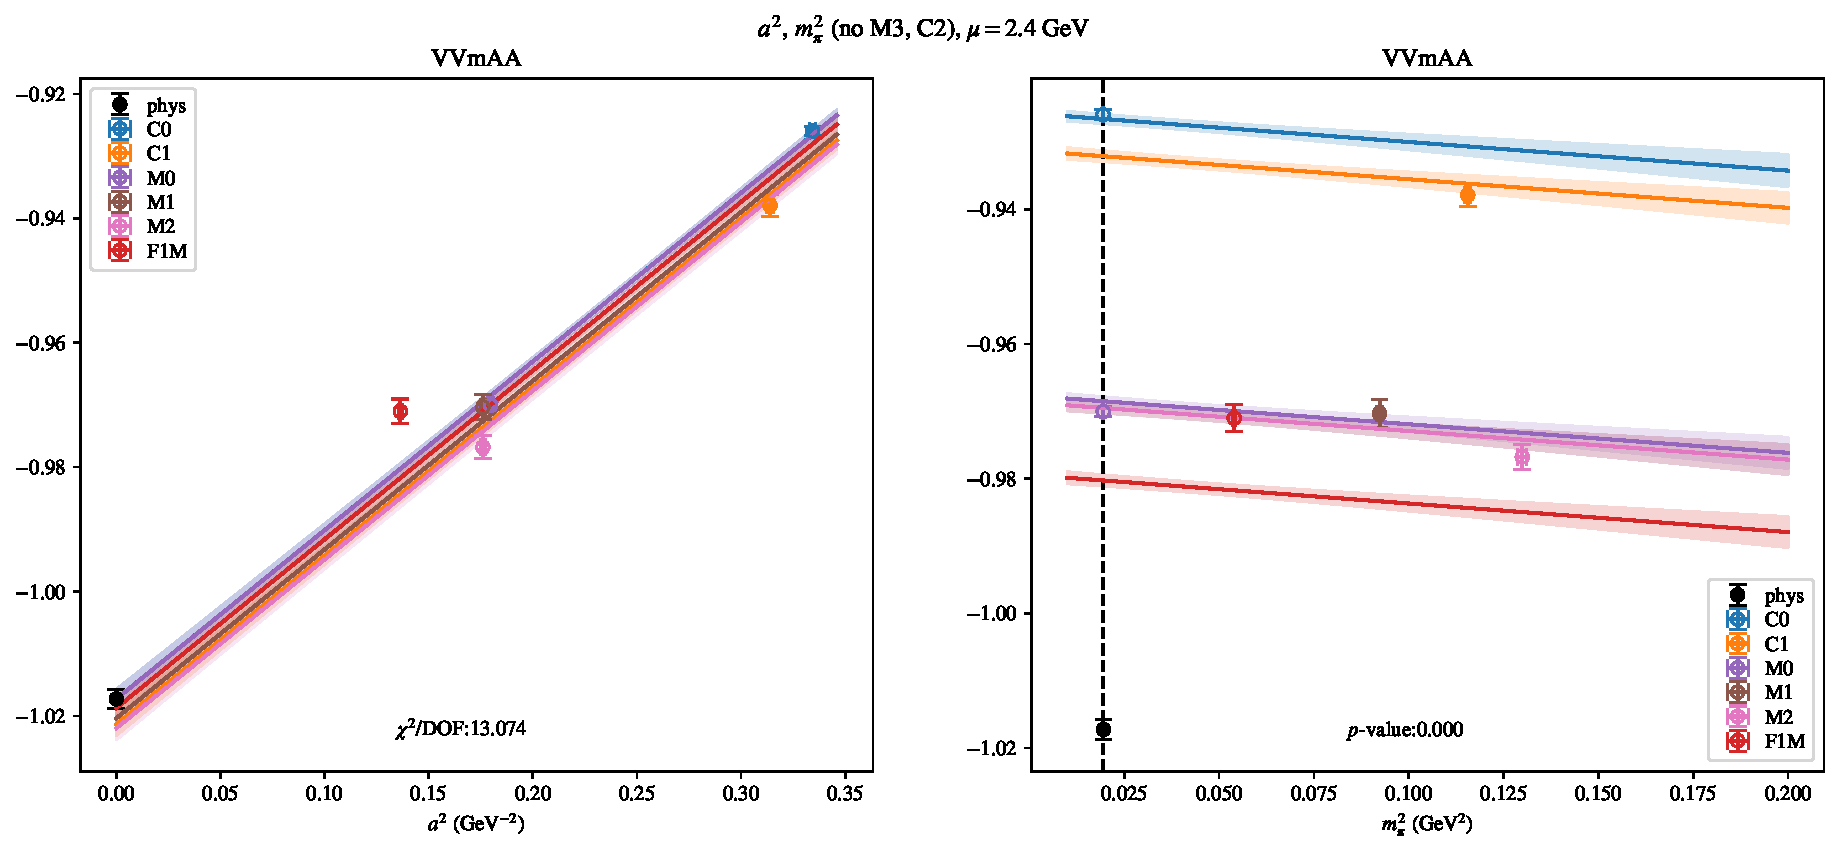
\includepdf[link, pages=-]{VVmAA/NPR/a2m2mcut_24.pdf}
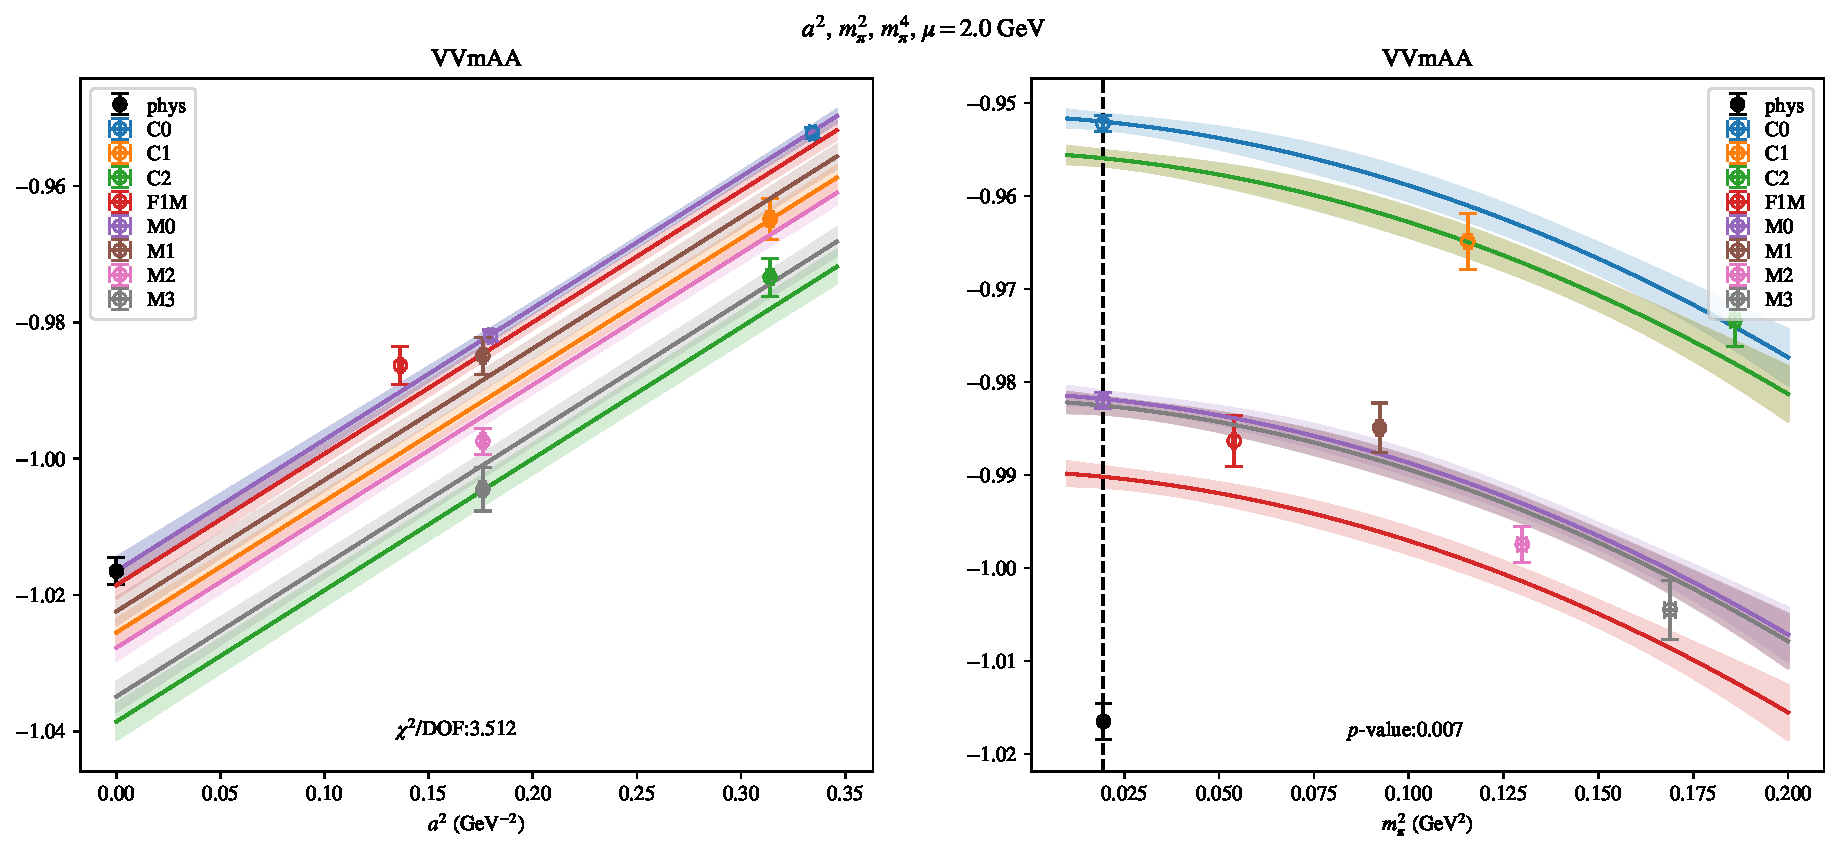
\includepdf[link, pages=-]{VVmAA/NPR/a2m2m4_20.pdf}
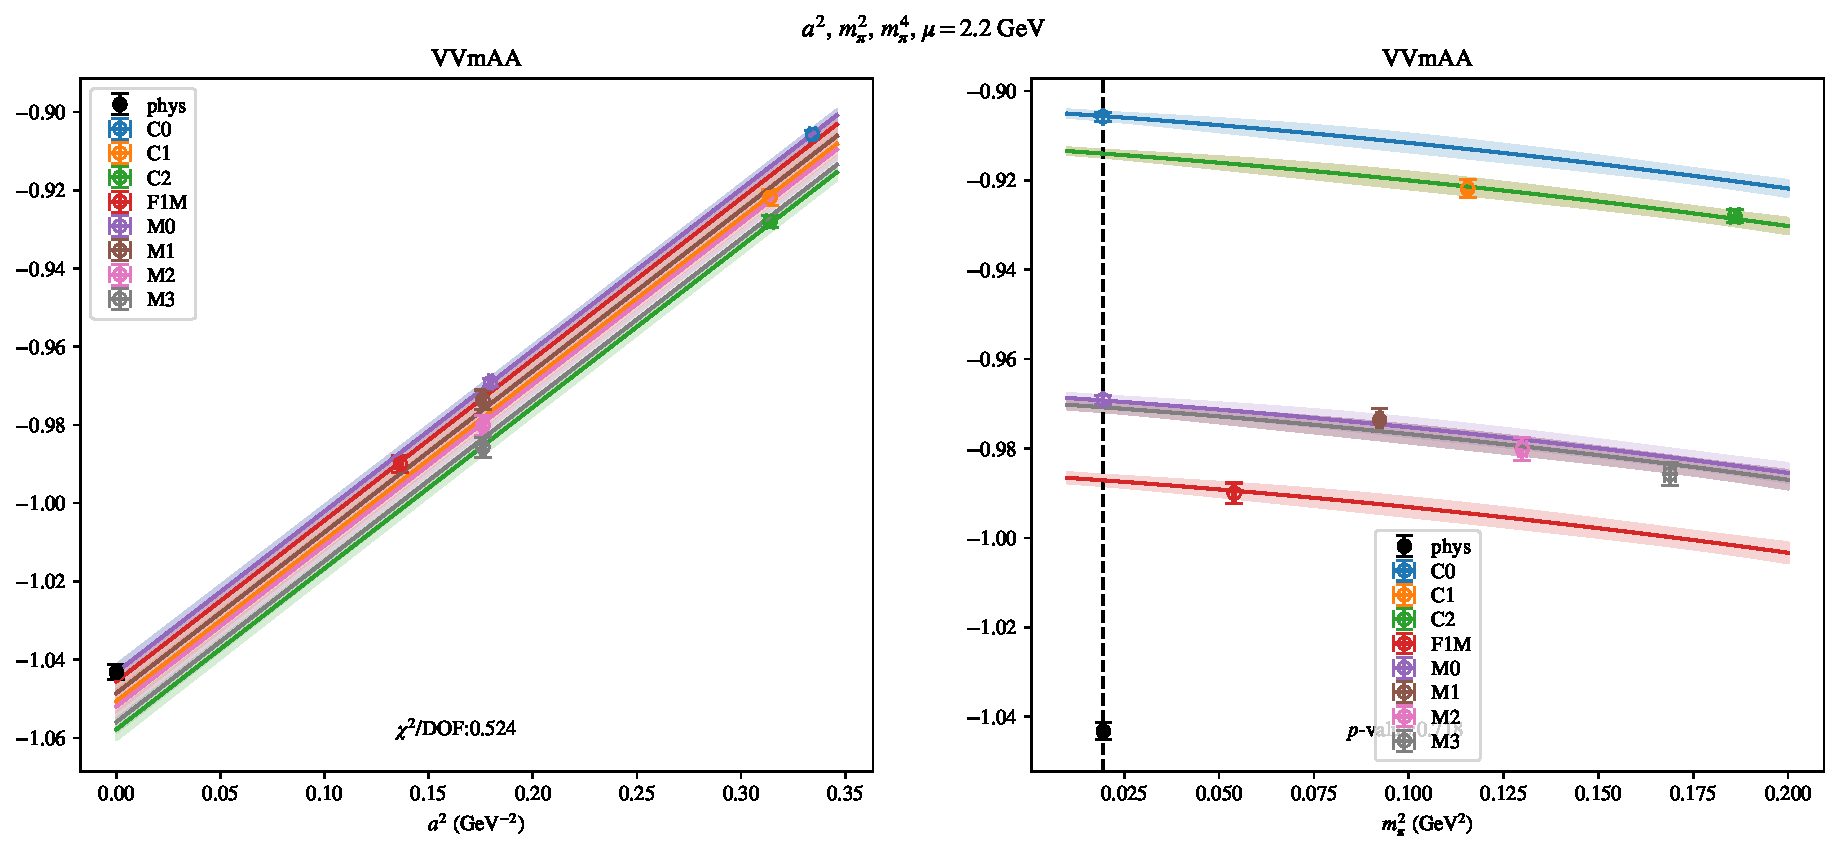
\includepdf[link, pages=-]{VVmAA/NPR/a2m2m4_22.pdf}
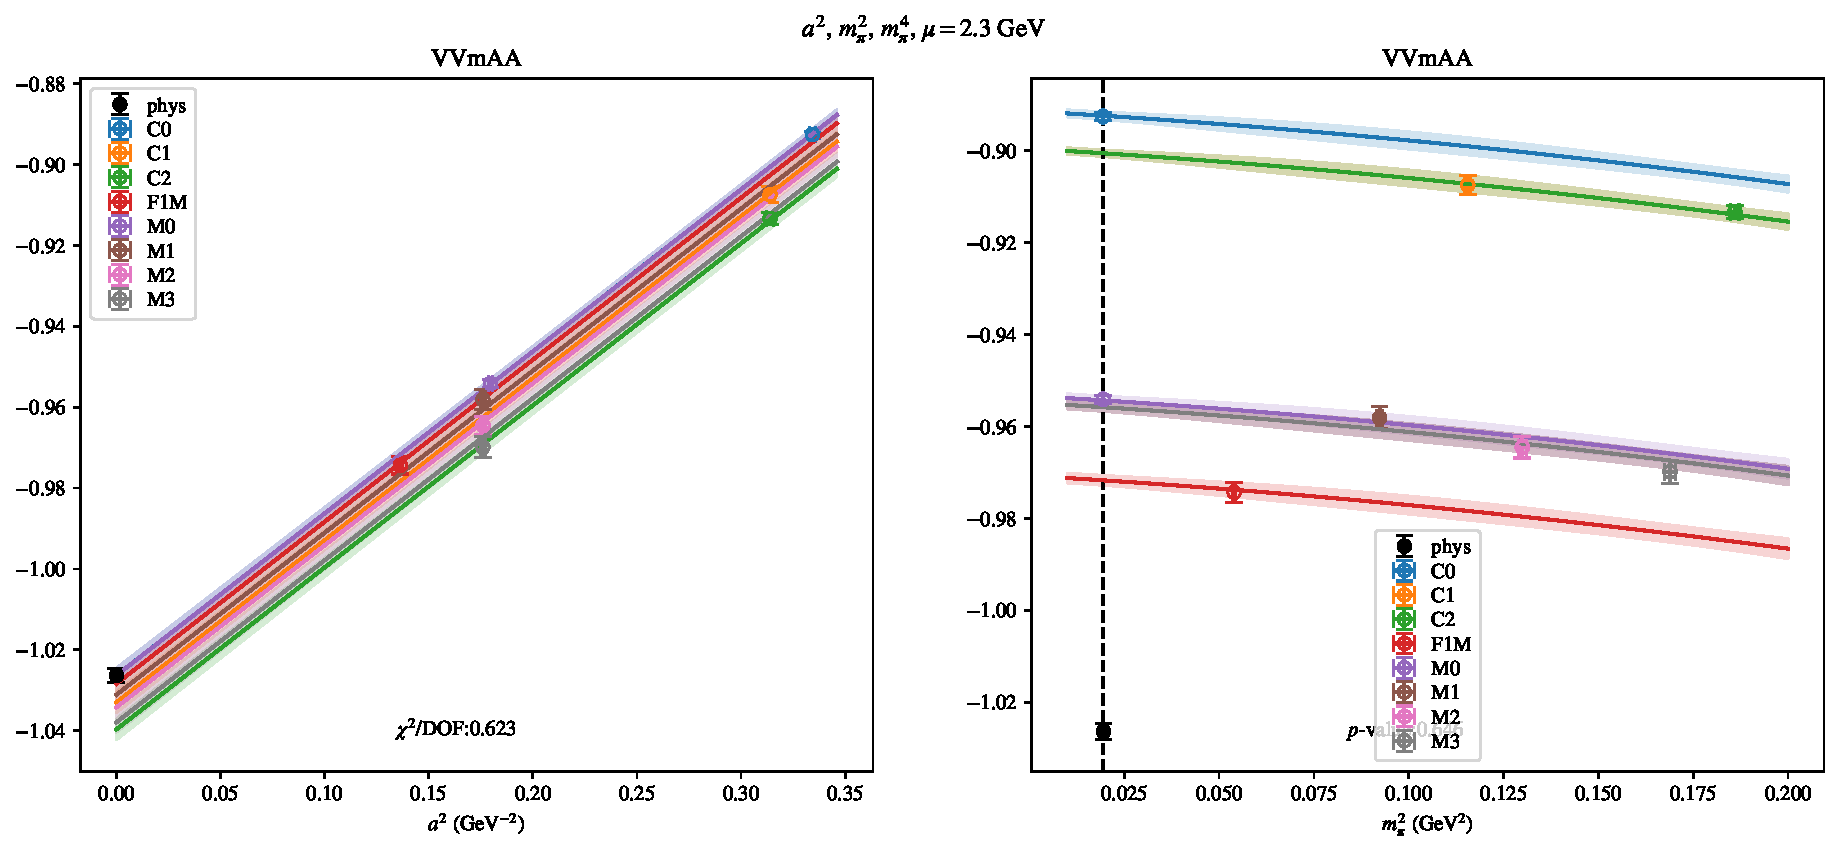
\includepdf[link, pages=-]{VVmAA/NPR/a2m2m4_23.pdf}
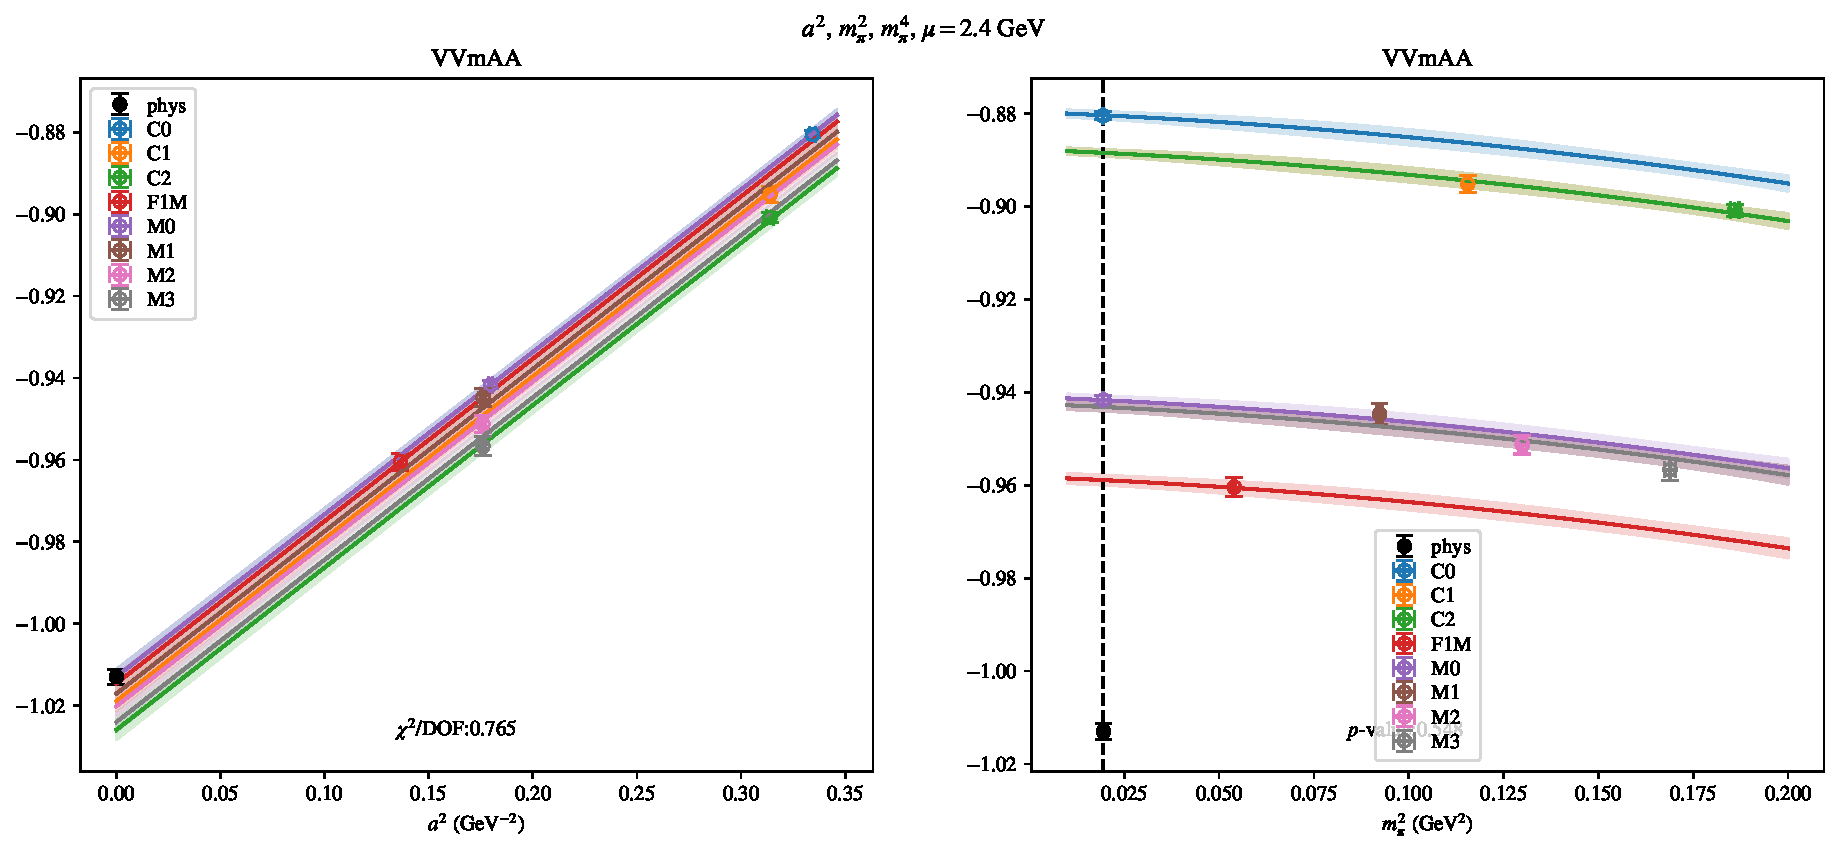
\includepdf[link, pages=-]{VVmAA/NPR/a2m2m4_24.pdf}
\clearpage
\section{$\mathcal{B}_3$}
\begin{table}[h!]
\begin{center}
\begin{tabular}{|c|c|c|c|c|c|}
\hline
$\mu$ (GeV) & $a^2$, $m_\pi^2$& $a^2$, $m_\pi^2$ (no C)& $a^2$, $a^4$, $m_\pi^2$& $a^2$, $m_\pi^2$ (no M3, C2)& $a^2$, $m_\pi^2$, $m_\pi^4$\\
\hline
2.0& \hyperlink{SSmPP/NPR/a2m2_20.pdf.1}{\textbf{1.8456(29)}: 5.613 (0.0)} & \hyperlink{SSmPP/NPR/a2m2noC_20.pdf.1}{\textbf{1.783(14)}: 3.031 (0.048)} & \hyperlink{SSmPP/NPR/a2a4m2_20.pdf.1}{\textbf{1.764(23)}: 3.814 (0.004)} & \hyperlink{SSmPP/NPR/a2m2mcut_20.pdf.1}{\textbf{1.8444(30)}: 6.739 (0.0)} & \hyperlink{SSmPP/NPR/a2m2m4_20.pdf.1}{\textbf{1.8484(31)}: 5.811 (0.0)}\\
2.2& \hyperlink{SSmPP/NPR/a2m2_22.pdf.1}{\textbf{1.8337(27)}: 5.365 (0.0)} & \hyperlink{SSmPP/NPR/a2m2noC_22.pdf.1}{\textbf{1.772(13)}: 2.002 (0.135)} & \hyperlink{SSmPP/NPR/a2a4m2_22.pdf.1}{\textbf{1.737(21)}: 1.481 (0.205)} & \hyperlink{SSmPP/NPR/a2m2mcut_22.pdf.1}{\textbf{1.8339(29)}: 7.9 (0.0)} & \hyperlink{SSmPP/NPR/a2m2m4_22.pdf.1}{\textbf{1.8370(29)}: 5.162 (0.0)}\\
2.3& \hyperlink{SSmPP/NPR/a2m2_23.pdf.1}{\textbf{1.8308(27)}: 5.66 (0.0)} & \hyperlink{SSmPP/NPR/a2m2noC_23.pdf.1}{\textbf{1.767(13)}: 2.047 (0.129)} & \hyperlink{SSmPP/NPR/a2a4m2_23.pdf.1}{\textbf{1.733(22)}: 1.793 (0.127)} & \hyperlink{SSmPP/NPR/a2m2mcut_23.pdf.1}{\textbf{1.8308(29)}: 8.241 (0.0)} & \hyperlink{SSmPP/NPR/a2m2m4_23.pdf.1}{\textbf{1.8342(29)}: 5.46 (0.0)}\\
2.4& \hyperlink{SSmPP/NPR/a2m2_24.pdf.1}{\textbf{1.8285(26)}: 6.39 (0.0)} & \hyperlink{SSmPP/NPR/a2m2noC_24.pdf.1}{\textbf{1.762(13)}: 2.38 (0.093)} & \hyperlink{SSmPP/NPR/a2a4m2_24.pdf.1}{\textbf{1.725(22)}: 1.933 (0.102)} & \hyperlink{SSmPP/NPR/a2m2mcut_24.pdf.1}{\textbf{1.8287(29)}: 9.333 (0.0)} & \hyperlink{SSmPP/NPR/a2m2m4_24.pdf.1}{\textbf{1.8322(29)}: 6.127 (0.0)}\\
\hline
\end{tabular}
\caption{Physical point value from chiral and continuum extrapolation at renormalisation scale $\mu$. Entries are \textbf{value(error)}: $\chi^2/\text{DOF}$ ($p$-value).}
\end{center}
\end{table}
\begin{table}[h!]
\begin{center}
\begin{tabular}{|c c|c|c|c|c|c|}
\hline
$\mu$ (GeV) &  & $a^2$, $m_\pi^2$& $a^2$, $m_\pi^2$ (no C)& $a^2$, $a^4$, $m_\pi^2$& $a^2$, $m_\pi^2$ (no M3, C2)& $a^2$, $m_\pi^2$, $m_\pi^4$\\
\hline
\multirow{2}{0.5in}{2.0} & $\alpha$ & 0.0622(60)& 0.261(48)& 0.47(12)& 0.0652(63)& 0.0571(64)\\
 & $\beta$ & -0.0002(15)& 0.00012(21)& -0.0003(15)& -0.0003(22)& -0.0018(66)\\
\hline
\multirow{2}{0.5in}{2.2} & $\alpha$ & 0.0706(56)& 0.273(45)& 0.57(12)& 0.0709(60)& 0.0647(61)\\
 & $\beta$ & -0.0002(12)& -0.0002(21)& -0.0004(13)& -0.0004(20)& -0.0018(60)\\
\hline
\multirow{2}{0.5in}{2.3} & $\alpha$ & 0.0713(56)& 0.281(45)& 0.58(12)& 0.0719(60)& 0.0651(60)\\
 & $\beta$ & -0.0003(12)& -0.0002(20)& -0.0005(13)& -0.0005(20)& -0.0020(62)\\
\hline
\multirow{2}{0.5in}{2.4} & $\alpha$ & 0.0722(55)& 0.292(45)& 0.61(12)& 0.0724(60)& 0.0655(60)\\
 & $\beta$ & -0.0003(12)& -0.0003(20)& -0.0005(13)& -0.0006(20)& -0.0021(61)\\
\hline
\end{tabular}
\caption{Fit values of coefficients in $Q = Q_{phys} + \mathbf{\alpha} a^2 + \mathbf{\beta}\left(\frac{m_\pi^2}{f_\pi^2}-\frac{m_{\pi,PDG}^2}{f_\pi^2}\right) + \ldots$.}
\end{center}
\end{table}
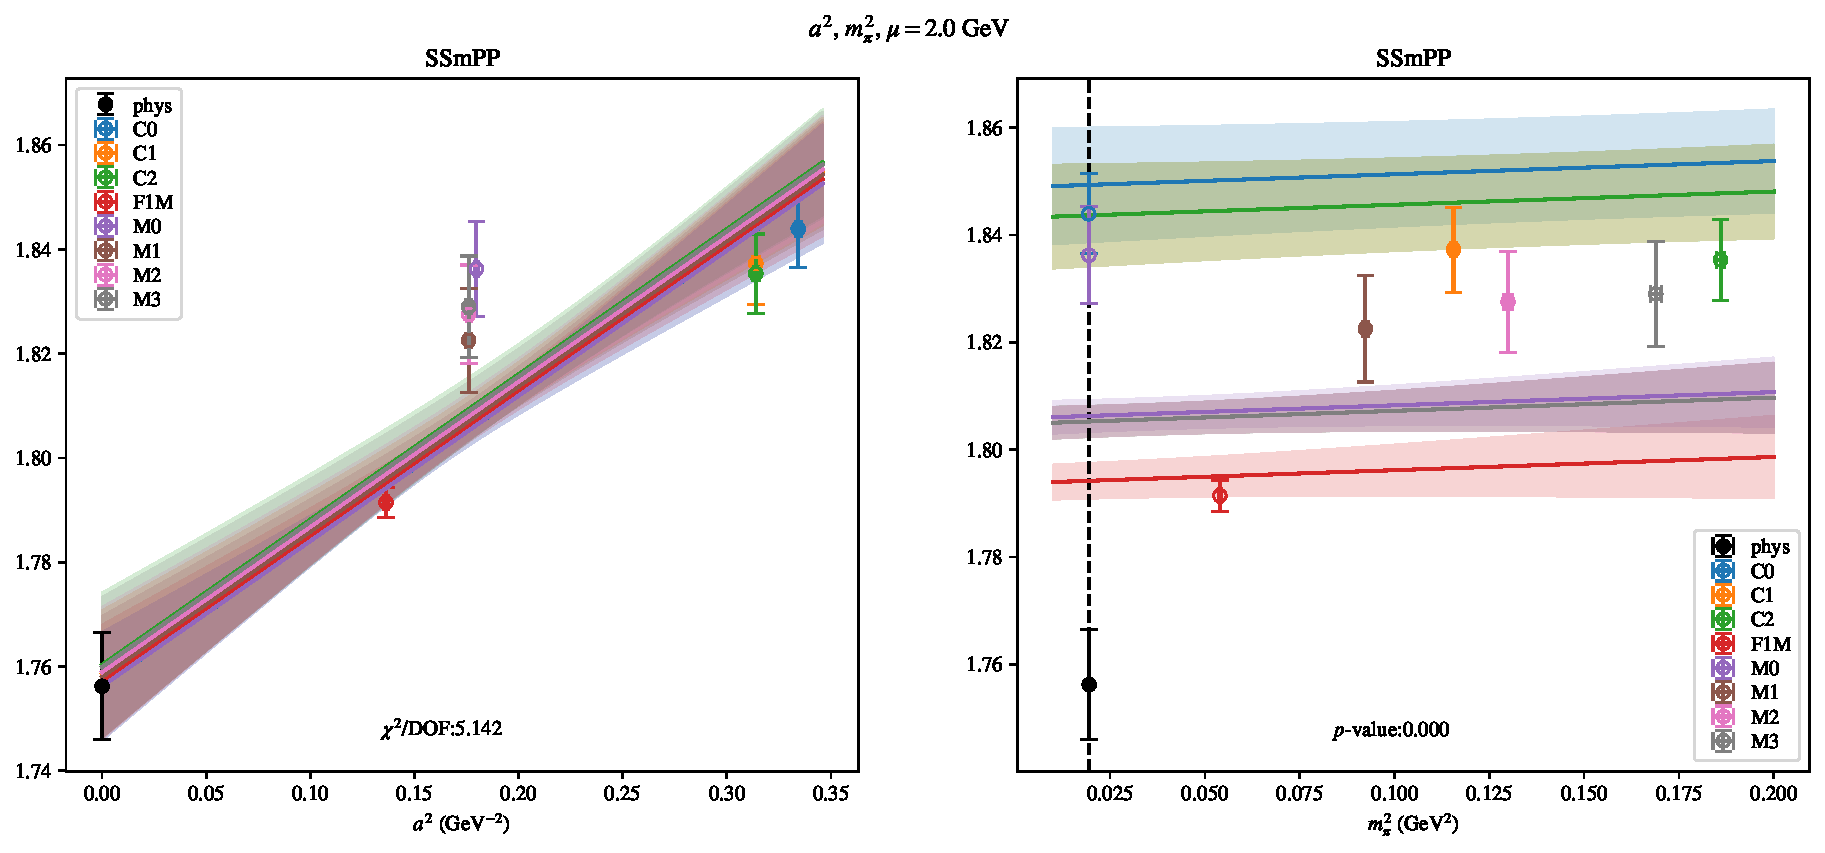
\includepdf[link, pages=-]{SSmPP/NPR/a2m2_20.pdf}
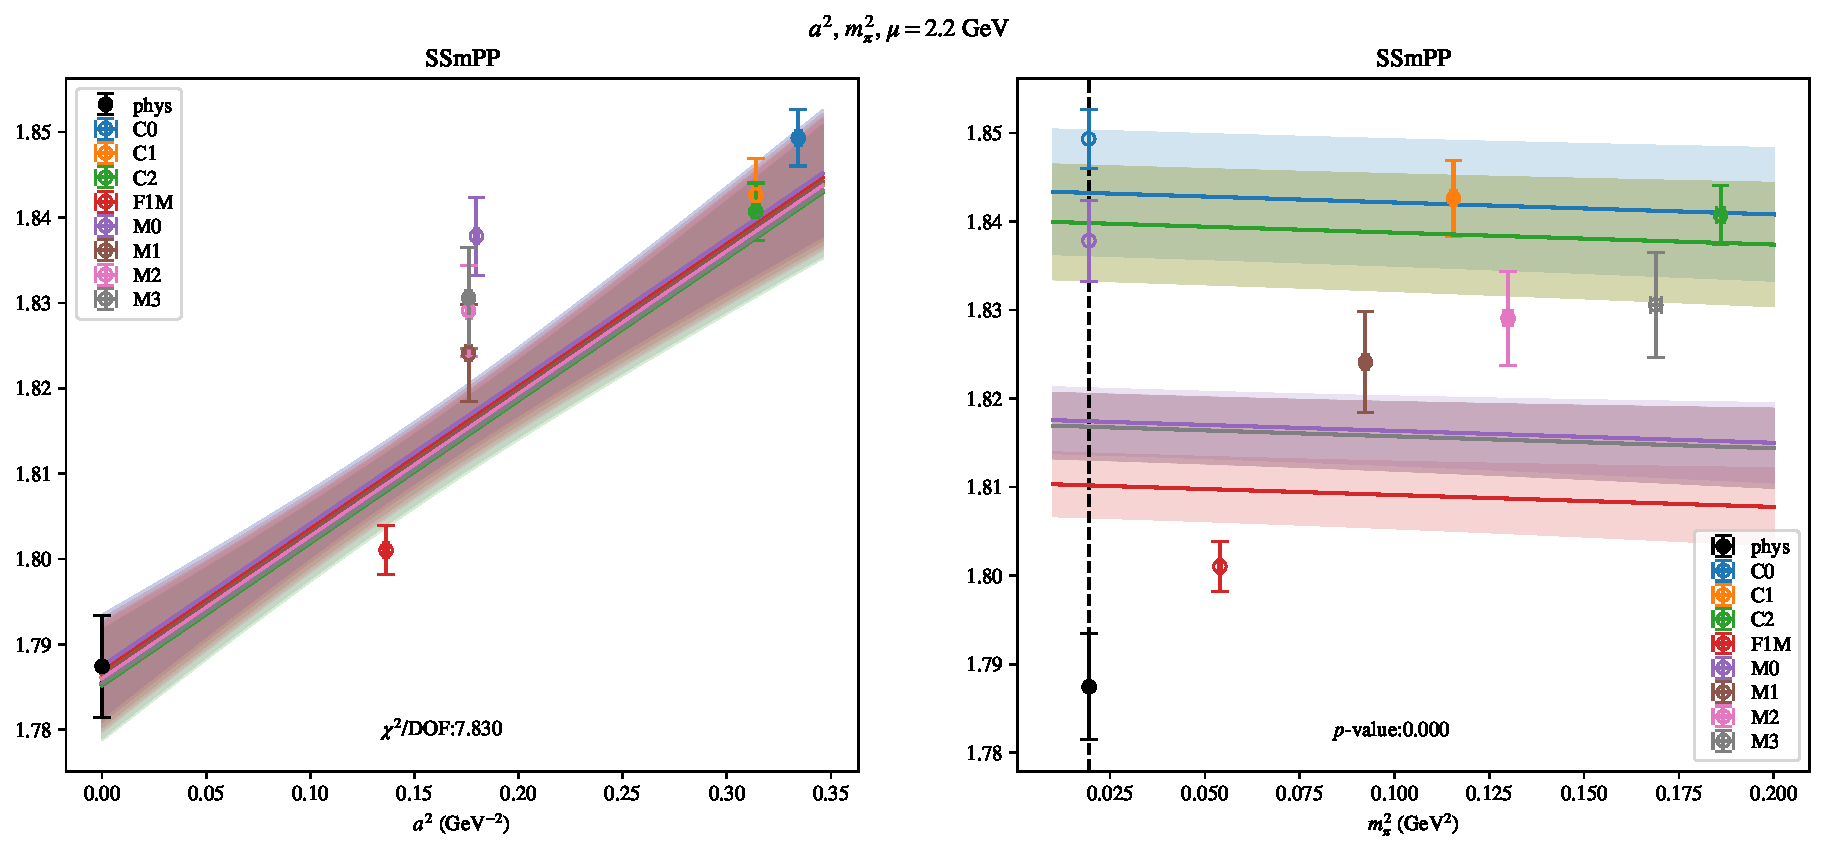
\includepdf[link, pages=-]{SSmPP/NPR/a2m2_22.pdf}
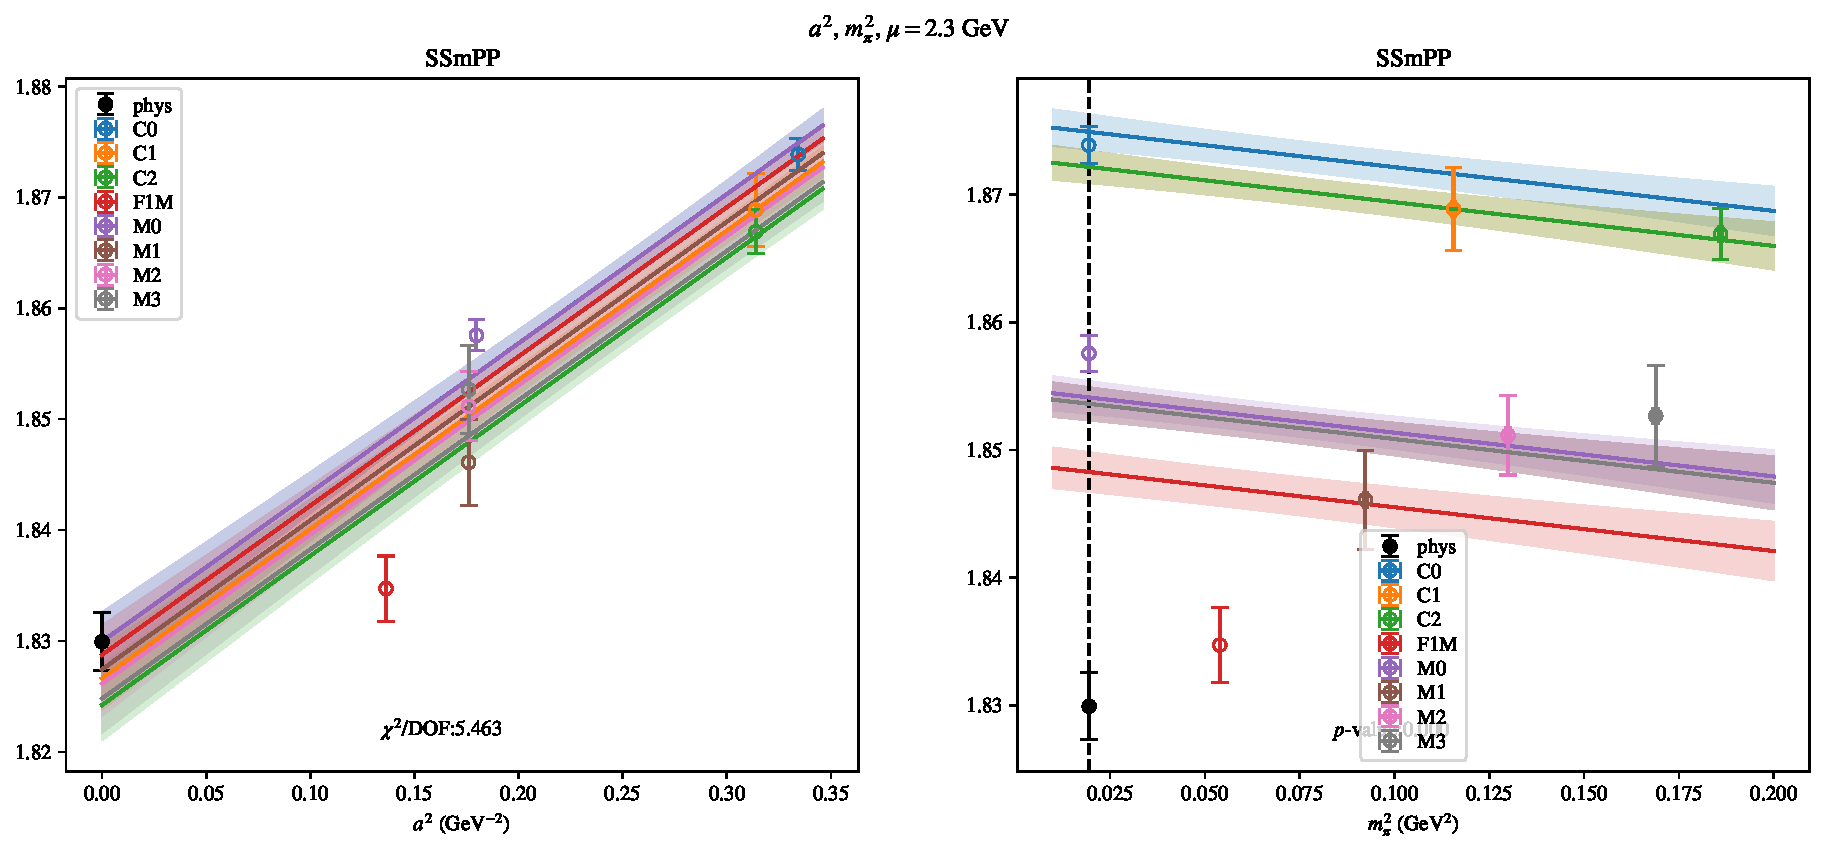
\includepdf[link, pages=-]{SSmPP/NPR/a2m2_23.pdf}
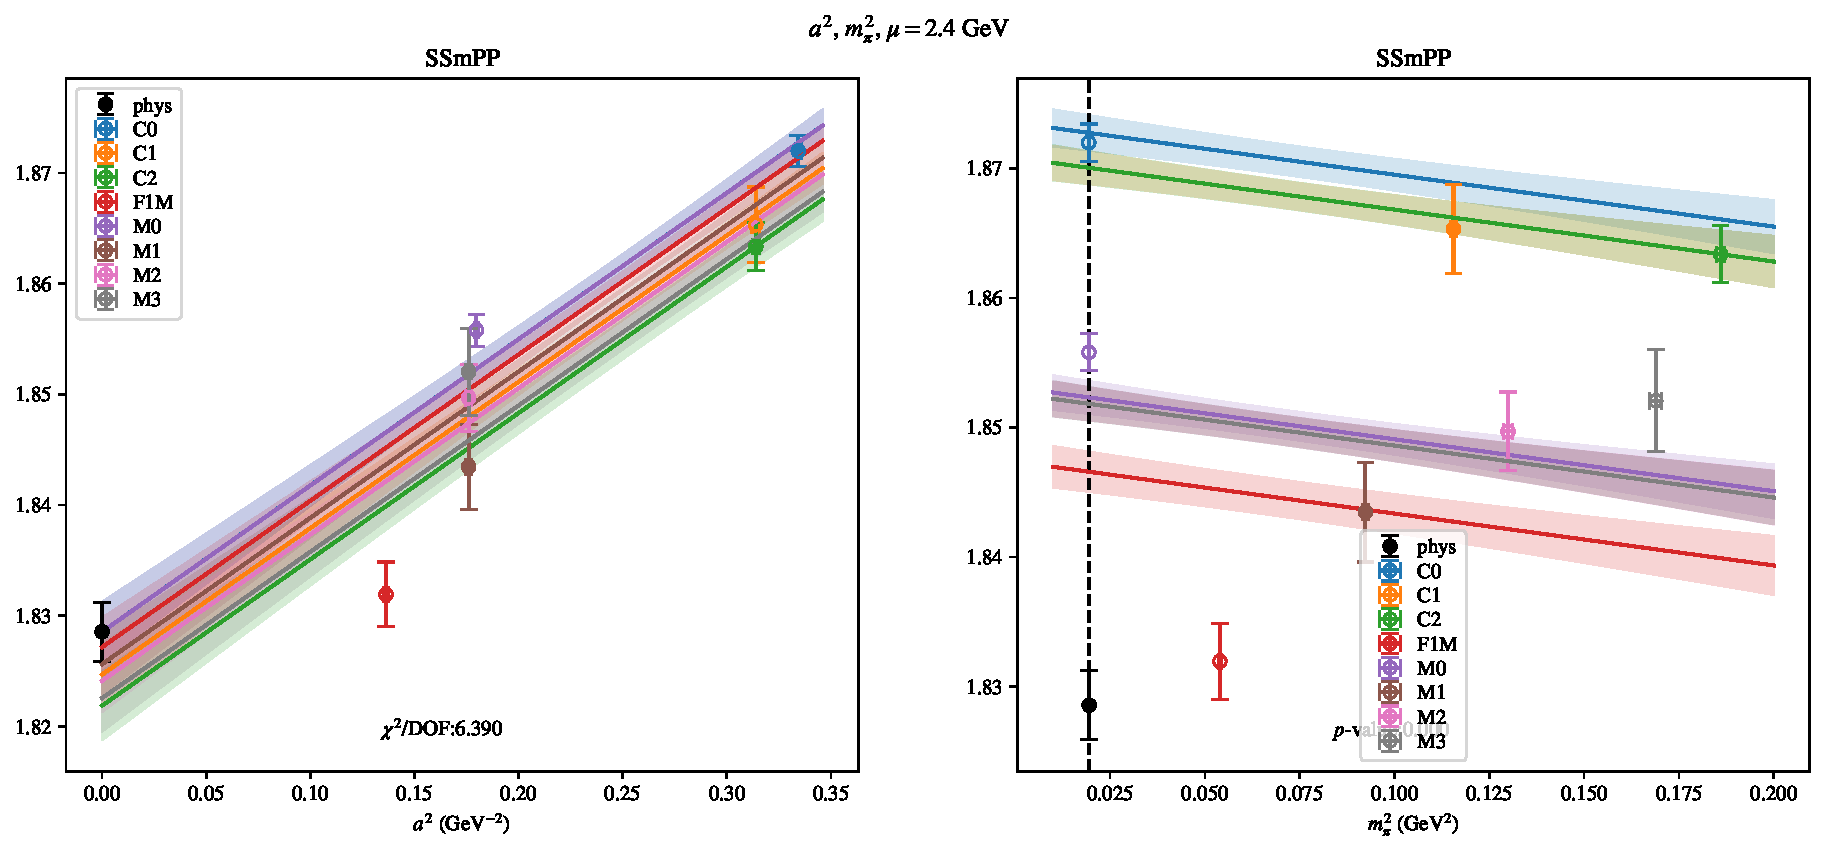
\includepdf[link, pages=-]{SSmPP/NPR/a2m2_24.pdf}
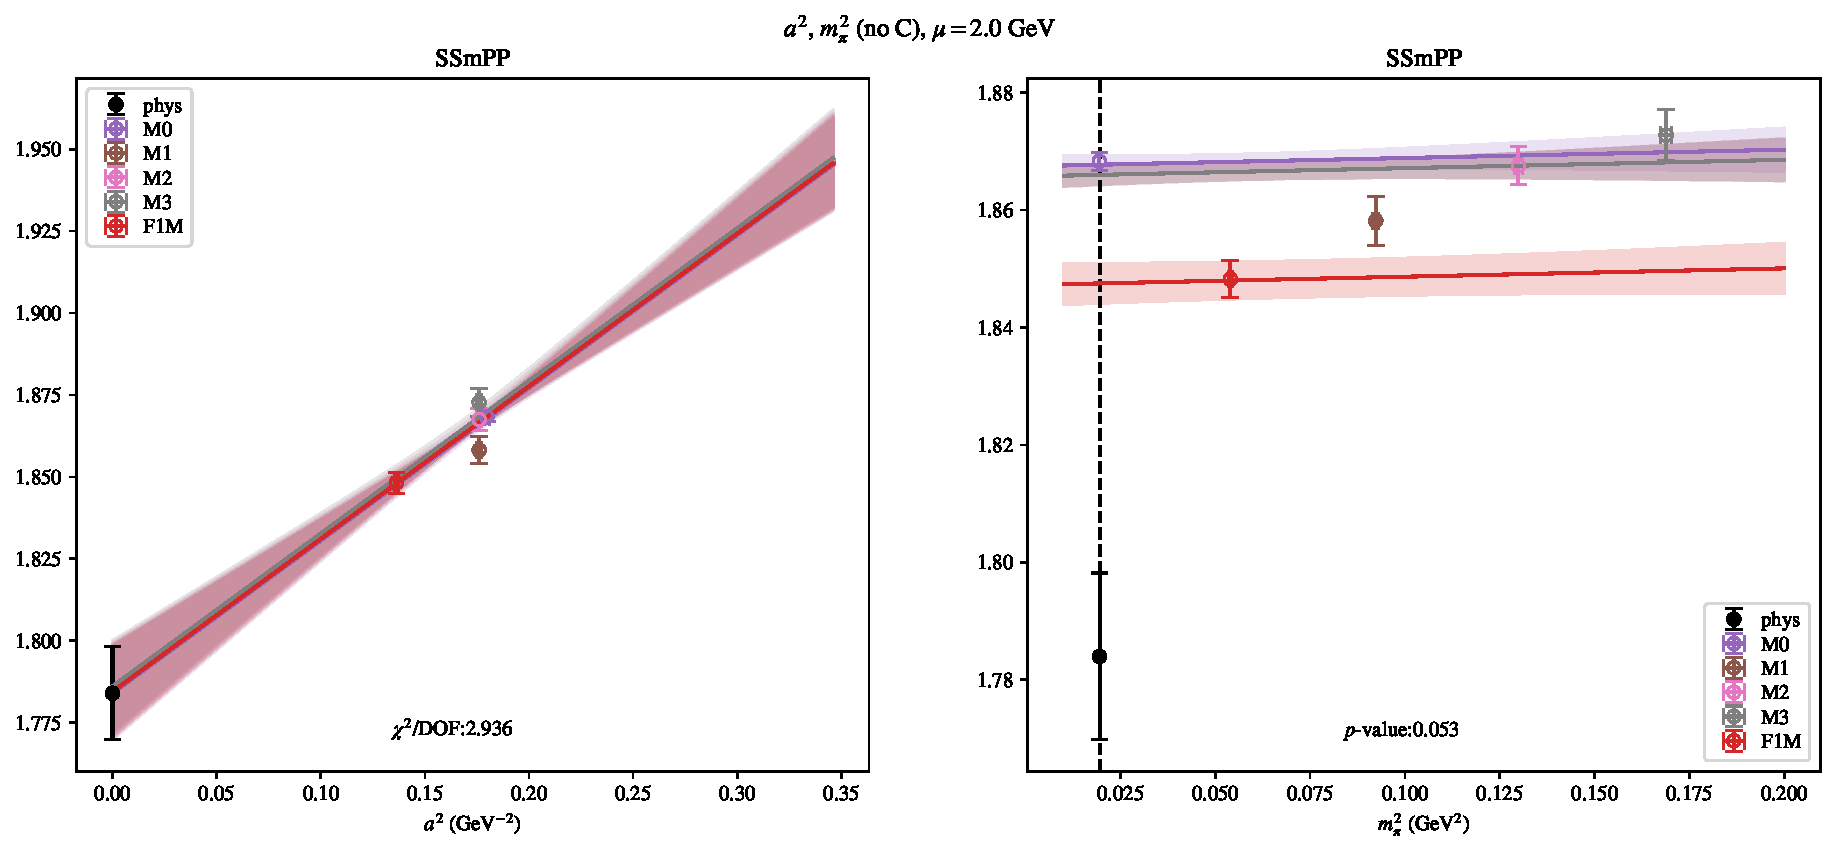
\includepdf[link, pages=-]{SSmPP/NPR/a2m2noC_20.pdf}
\includepdf[link, pages=-]{SSmPP/NPR/a2m2noC_22.pdf}
\includepdf[link, pages=-]{SSmPP/NPR/a2m2noC_23.pdf}
\includepdf[link, pages=-]{SSmPP/NPR/a2m2noC_24.pdf}
\includepdf[link, pages=-]{SSmPP/NPR/a2a4m2_20.pdf}
\includepdf[link, pages=-]{SSmPP/NPR/a2a4m2_22.pdf}
\includepdf[link, pages=-]{SSmPP/NPR/a2a4m2_23.pdf}
\includepdf[link, pages=-]{SSmPP/NPR/a2a4m2_24.pdf}
\includepdf[link, pages=-]{SSmPP/NPR/a2m2mcut_20.pdf}
\includepdf[link, pages=-]{SSmPP/NPR/a2m2mcut_22.pdf}
\includepdf[link, pages=-]{SSmPP/NPR/a2m2mcut_23.pdf}
\includepdf[link, pages=-]{SSmPP/NPR/a2m2mcut_24.pdf}
\includepdf[link, pages=-]{SSmPP/NPR/a2m2m4_20.pdf}
\includepdf[link, pages=-]{SSmPP/NPR/a2m2m4_22.pdf}
\includepdf[link, pages=-]{SSmPP/NPR/a2m2m4_23.pdf}
\includepdf[link, pages=-]{SSmPP/NPR/a2m2m4_24.pdf}
\clearpage
\section{$\mathcal{B}_4$}
\begin{table}[h!]
\begin{center}
\begin{tabular}{|c|c|c|c|c|c|}
\hline
$\mu$ (GeV) & $a^2$, $m_\pi^2$& $a^2$, $m_\pi^2$ (no C)& $a^2$, $a^4$, $m_\pi^2$& $a^2$, $m_\pi^2$ (no M3, C2)& $a^2$, $m_\pi^2$, $m_\pi^4$\\
\hline
2.0& \hyperlink{SSpPP/NPR/a2m2_20.pdf.1}{\textbf{-0.949(21)}: 3.549 (0.003)} & \hyperlink{SSpPP/NPR/a2m2noC_20.pdf.1}{\textbf{-0.98(10)}: 1.041 (0.353)} & \hyperlink{SSpPP/NPR/a2a4m2_20.pdf.1}{\textbf{-1.00(17)}: 1.373 (0.241)} & \hyperlink{SSpPP/NPR/a2m2mcut_20.pdf.1}{\textbf{-0.948(23)}: 5.331 (0.001)} & \hyperlink{SSpPP/NPR/a2m2m4_20.pdf.1}{\textbf{-0.946(24)}: 2.787 (0.025)}\\
2.2& \hyperlink{SSpPP/NPR/a2m2_22.pdf.1}{\textbf{-0.920(19)}: 4.953 (0.0)} & \hyperlink{SSpPP/NPR/a2m2noC_22.pdf.1}{\textbf{-0.956(96)}: 1.737 (0.176)} & \hyperlink{SSpPP/NPR/a2a4m2_22.pdf.1}{\textbf{-0.96(15)}: 4.191 (0.002)} & \hyperlink{SSpPP/NPR/a2m2mcut_22.pdf.1}{\textbf{-0.920(20)}: 6.921 (0.0)} & \hyperlink{SSpPP/NPR/a2m2m4_22.pdf.1}{\textbf{-0.918(21)}: 4.585 (0.001)}\\
2.3& \hyperlink{SSpPP/NPR/a2m2_23.pdf.1}{\textbf{-0.908(18)}: 4.67 (0.0)} & \hyperlink{SSpPP/NPR/a2m2noC_23.pdf.1}{\textbf{-0.944(94)}: 1.662 (0.19)} & \hyperlink{SSpPP/NPR/a2a4m2_23.pdf.1}{\textbf{-0.95(15)}: 3.692 (0.005)} & \hyperlink{SSpPP/NPR/a2m2mcut_23.pdf.1}{\textbf{-0.908(20)}: 6.507 (0.0)} & \hyperlink{SSpPP/NPR/a2m2m4_23.pdf.1}{\textbf{-0.906(20)}: 4.189 (0.002)}\\
2.4& \hyperlink{SSpPP/NPR/a2m2_24.pdf.1}{\textbf{-0.899(18)}: 4.561 (0.0)} & \hyperlink{SSpPP/NPR/a2m2noC_24.pdf.1}{\textbf{-0.931(92)}: 1.53 (0.216)} & \hyperlink{SSpPP/NPR/a2a4m2_24.pdf.1}{\textbf{-0.93(15)}: 4.245 (0.002)} & \hyperlink{SSpPP/NPR/a2m2mcut_24.pdf.1}{\textbf{-0.899(19)}: 6.242 (0.0)} & \hyperlink{SSpPP/NPR/a2m2m4_24.pdf.1}{\textbf{-0.897(20)}: 4.387 (0.002)}\\
\hline
\end{tabular}
\caption{Physical point value from chiral and continuum extrapolation at renormalisation scale $\mu$. Entries are \textbf{value(error)}: $\chi^2/\text{DOF}$ ($p$-value).}
\end{center}
\end{table}
\begin{table}[h!]
\begin{center}
\begin{tabular}{|c c|c|c|c|c|c|}
\hline
$\mu$ (GeV) &  & $a^2$, $m_\pi^2$& $a^2$, $m_\pi^2$ (no C)& $a^2$, $a^4$, $m_\pi^2$& $a^2$, $m_\pi^2$ (no M3, C2)& $a^2$, $m_\pi^2$, $m_\pi^4$\\
\hline
\multirow{2}{0.5in}{2.0} & $\alpha$ & 0.3672(94)& 0.130(64)& -0.1(15)& 0.3717(99)& 0.377(10)\\
 & $\beta$ & 0.00744(23)& 0.00722(27)& 0.00717(24)& 0.00778(34)& 0.01005(95)\\
\hline
\multirow{2}{0.5in}{2.2} & $\alpha$ & 0.4152(89)& 0.184(60)& -0.008& 0.4146(95)& 0.4244(97)\\
 & $\beta$ & 0.00752(21)& 0.00689(24)& 0.00732(22)& 0.00783(30)& 0.00984(85)\\
\hline
\multirow{2}{0.5in}{2.3} & $\alpha$ & 0.4364(88)& 0.206(60)& 0.004& 0.4360(93)& 0.4450(95)\\
 & $\beta$ & 0.00746(21)& 0.00687(24)& 0.00725(22)& 0.00778(31)& 0.00982(86)\\
\hline
\multirow{2}{0.5in}{2.4} & $\alpha$ & 0.4541(85)& 0.244(60)& 0.099& 0.4529(91)& 0.4620(93)\\
 & $\beta$ & 0.00749(19)& 0.00685(24)& 0.00732(21)& 0.00776(30)& 0.00948(83)\\
\hline
\end{tabular}
\caption{Fit values of coefficients in $Q = Q_{phys} + \mathbf{\alpha} a^2 + \mathbf{\beta}\left(\frac{m_\pi^2}{f_\pi^2}-\frac{m_{\pi,PDG}^2}{f_\pi^2}\right) + \ldots$.}
\end{center}
\end{table}
\includepdf[link, pages=-]{SSpPP/NPR/a2m2_20.pdf}
\includepdf[link, pages=-]{SSpPP/NPR/a2m2_22.pdf}
\includepdf[link, pages=-]{SSpPP/NPR/a2m2_23.pdf}
\includepdf[link, pages=-]{SSpPP/NPR/a2m2_24.pdf}
\includepdf[link, pages=-]{SSpPP/NPR/a2m2noC_20.pdf}
\includepdf[link, pages=-]{SSpPP/NPR/a2m2noC_22.pdf}
\includepdf[link, pages=-]{SSpPP/NPR/a2m2noC_23.pdf}
\includepdf[link, pages=-]{SSpPP/NPR/a2m2noC_24.pdf}
\includepdf[link, pages=-]{SSpPP/NPR/a2a4m2_20.pdf}
\includepdf[link, pages=-]{SSpPP/NPR/a2a4m2_22.pdf}
\includepdf[link, pages=-]{SSpPP/NPR/a2a4m2_23.pdf}
\includepdf[link, pages=-]{SSpPP/NPR/a2a4m2_24.pdf}
\includepdf[link, pages=-]{SSpPP/NPR/a2m2mcut_20.pdf}
\includepdf[link, pages=-]{SSpPP/NPR/a2m2mcut_22.pdf}
\includepdf[link, pages=-]{SSpPP/NPR/a2m2mcut_23.pdf}
\includepdf[link, pages=-]{SSpPP/NPR/a2m2mcut_24.pdf}
\includepdf[link, pages=-]{SSpPP/NPR/a2m2m4_20.pdf}
\includepdf[link, pages=-]{SSpPP/NPR/a2m2m4_22.pdf}
\includepdf[link, pages=-]{SSpPP/NPR/a2m2m4_23.pdf}
\includepdf[link, pages=-]{SSpPP/NPR/a2m2m4_24.pdf}
\clearpage
\section{$\mathcal{B}_5$}
\begin{table}[h!]
\begin{center}
\begin{tabular}{|c|c|c|c|c|c|}
\hline
$\mu$ (GeV) & $a^2$, $m_\pi^2$& $a^2$, $m_\pi^2$ (no C)& $a^2$, $a^4$, $m_\pi^2$& $a^2$, $m_\pi^2$ (no M3, C2)& $a^2$, $m_\pi^2$, $m_\pi^4$\\
\hline
2.0& \hyperlink{TT/NPR/a2m2_20.pdf.1}{\textbf{-0.370(10)}: 1.19 (0.311)} & \hyperlink{TT/NPR/a2m2noC_20.pdf.1}{\textbf{-0.383(57)}: 0.123 (0.885)} & \hyperlink{TT/NPR/a2a4m2_20.pdf.1}{\textbf{-0.391(95)}: 0.167 (0.955)} & \hyperlink{TT/NPR/a2m2mcut_20.pdf.1}{\textbf{-0.370(10)}: 1.892 (0.128)} & \hyperlink{TT/NPR/a2m2m4_20.pdf.1}{\textbf{-0.370(10)}: 1.329 (0.256)}\\
2.2& \hyperlink{TT/NPR/a2m2_22.pdf.1}{\textbf{-0.3653(88)}: 1.697 (0.131)} & \hyperlink{TT/NPR/a2m2noC_22.pdf.1}{\textbf{-0.376(43)}: 0.143 (0.867)} & \hyperlink{TT/NPR/a2a4m2_22.pdf.1}{\textbf{-0.380(68)}: 0.824 (0.509)} & \hyperlink{TT/NPR/a2m2mcut_22.pdf.1}{\textbf{-0.3654(89)}: 2.751 (0.041)} & \hyperlink{TT/NPR/a2m2m4_22.pdf.1}{\textbf{-0.3650(92)}: 1.955 (0.098)}\\
2.3& \hyperlink{TT/NPR/a2m2_23.pdf.1}{\textbf{-0.3631(88)}: 1.476 (0.194)} & \hyperlink{TT/NPR/a2m2noC_23.pdf.1}{\textbf{-0.373(42)}: 0.139 (0.87)} & \hyperlink{TT/NPR/a2a4m2_23.pdf.1}{\textbf{-0.377(69)}: 0.749 (0.559)} & \hyperlink{TT/NPR/a2m2mcut_23.pdf.1}{\textbf{-0.3631(87)}: 2.348 (0.071)} & \hyperlink{TT/NPR/a2m2m4_23.pdf.1}{\textbf{-0.3627(91)}: 1.638 (0.162)}\\
2.4& \hyperlink{TT/NPR/a2m2_24.pdf.1}{\textbf{-0.3612(82)}: 1.294 (0.263)} & \hyperlink{TT/NPR/a2m2noC_24.pdf.1}{\textbf{-0.370(42)}: 0.183 (0.833)} & \hyperlink{TT/NPR/a2a4m2_24.pdf.1}{\textbf{-0.372(67)}: 0.926 (0.448)} & \hyperlink{TT/NPR/a2m2mcut_24.pdf.1}{\textbf{-0.3613(82)}: 2.022 (0.108)} & \hyperlink{TT/NPR/a2m2m4_24.pdf.1}{\textbf{-0.3610(85)}: 1.481 (0.205)}\\
\hline
\end{tabular}
\caption{Physical point value from chiral and continuum extrapolation at renormalisation scale $\mu$. Entries are \textbf{value(error)}: $\chi^2/\text{DOF}$ ($p$-value).}
\end{center}
\end{table}
\begin{table}[h!]
\begin{center}
\begin{tabular}{|c c|c|c|c|c|c|}
\hline
$\mu$ (GeV) &  & $a^2$, $m_\pi^2$& $a^2$, $m_\pi^2$ (no C)& $a^2$, $a^4$, $m_\pi^2$& $a^2$, $m_\pi^2$ (no M3, C2)& $a^2$, $m_\pi^2$, $m_\pi^4$\\
\hline
\multirow{2}{0.5in}{2.0} & $\alpha$ & -0.03(10)& -0.23(81)& -0.5(20)& -0.03(10)& -0.03(10)\\
 & $\beta$ & 0.00708(35)& 0.00684(37)& 0.00679(36)& 0.00713(41)& 0.0081(12)\\
\hline
\multirow{2}{0.5in}{2.2} & $\alpha$ & -0.084(92)& -0.25(63)& -0.4(15)& -0.086(93)& -0.082(96)\\
 & $\beta$ & 0.00681(26)& 0.00642(28)& 0.00660(28)& 0.00680(32)& 0.00765(92)\\
\hline
\multirow{2}{0.5in}{2.3} & $\alpha$ & -0.108(91)& -0.26(62)& -0.4(15)& -0.109(91)& -0.105(94)\\
 & $\beta$ & 0.00675(26)& 0.00639(28)& 0.00656(28)& 0.00678(32)& 0.00769(95)\\
\hline
\multirow{2}{0.5in}{2.4} & $\alpha$ & -0.131(87)& -0.26(63)& -0.3(15)& -0.133(88)& -0.129(90)\\
 & $\beta$ & 0.00669(24)& 0.00635(26)& 0.00654(26)& 0.00670(30)& 0.00740(89)\\
\hline
\end{tabular}
\caption{Fit values of coefficients in $Q = Q_{phys} + \mathbf{\alpha} a^2 + \mathbf{\beta}\left(\frac{m_\pi^2}{f_\pi^2}-\frac{m_{\pi,PDG}^2}{f_\pi^2}\right) + \ldots$.}
\end{center}
\end{table}
\includepdf[link, pages=-]{TT/NPR/a2m2_20.pdf}
\includepdf[link, pages=-]{TT/NPR/a2m2_22.pdf}
\includepdf[link, pages=-]{TT/NPR/a2m2_23.pdf}
\includepdf[link, pages=-]{TT/NPR/a2m2_24.pdf}
\includepdf[link, pages=-]{TT/NPR/a2m2noC_20.pdf}
\includepdf[link, pages=-]{TT/NPR/a2m2noC_22.pdf}
\includepdf[link, pages=-]{TT/NPR/a2m2noC_23.pdf}
\includepdf[link, pages=-]{TT/NPR/a2m2noC_24.pdf}
\includepdf[link, pages=-]{TT/NPR/a2a4m2_20.pdf}
\includepdf[link, pages=-]{TT/NPR/a2a4m2_22.pdf}
\includepdf[link, pages=-]{TT/NPR/a2a4m2_23.pdf}
\includepdf[link, pages=-]{TT/NPR/a2a4m2_24.pdf}
\includepdf[link, pages=-]{TT/NPR/a2m2mcut_20.pdf}
\includepdf[link, pages=-]{TT/NPR/a2m2mcut_22.pdf}
\includepdf[link, pages=-]{TT/NPR/a2m2mcut_23.pdf}
\includepdf[link, pages=-]{TT/NPR/a2m2mcut_24.pdf}
\includepdf[link, pages=-]{TT/NPR/a2m2m4_20.pdf}
\includepdf[link, pages=-]{TT/NPR/a2m2m4_22.pdf}
\includepdf[link, pages=-]{TT/NPR/a2m2m4_23.pdf}
\includepdf[link, pages=-]{TT/NPR/a2m2m4_24.pdf}
\clearpage
\end{document}